% arXiv:2408.03314v1 的完整中文译稿; 译者说明明确与作者原文分开. 
\originalchapter{最优扩展大语言模型推理时计算可以比扩展模型参数更有效}
\label{testcompute-chapter}
\markboth{\thechapter\quad 推理时计算的最优扩展}{}
\begin{center}
Charlie Snell, Jaehoon Lee, Kelvin Xu, Aviral Kumar\\
原题: Scaling LLM Test-Time Compute Optimally can be More Effective than Scaling Model Parameters\\
arXiv:2408.03314v1, 2024 年 8 月 6 日
\end{center}
\begin{remark}
译者说明: Charlie Snell 任职于 UC Berkeley, 本工作完成于其在 Google DeepMind 实习期间; 其余作者任职于 Google DeepMind, Kelvin Xu 与 Aviral Kumar 共同指导. 通讯作者: \texttt{csnell22@berkeley.edu}. 原作依 CC BY 4.0 发布, \url{https://arxiv.org/abs/2408.03314v1}; 许可: \url{https://creativecommons.org/licenses/by/4.0/}. 中文翻译、结构适配与图中文字转写由 ai-self-study contributors 以机器辅助方式完成. 本译本统一将 test-time compute 和 inference-time compute 译为“推理时计算”（亦称“测试时计算”）. 正文中的“我们”均指原论文作者. 原作者图件保留, 图注和必要的图中文字另译; 模型错误输出照录, 不据数学常识修正. 译文依同一许可发布. 
\end{remark}

\originalsection{摘要}
\label{testcompute-abstract}
让大语言模型（LLM）通过使用更多推理时计算改进其输出, 是构建能够处理开放式自然语言、具有通用自我改进能力的智能体的关键一步. 本文研究 LLM 中推理时计算的扩展, 重点回答如下问题: \emph{如果允许一个 LLM 使用固定但非微不足道数量的推理时计算, 它能在一个具有挑战性的提示上将表现提高多少? } 回答这一问题, 不仅关系到 LLM 所能达到的表现, 也关系到 LLM 预训练的未来, 以及应如何权衡推理时计算与预训练计算. 尽管这一问题很重要, 尝试理解各种测试时推理方法的扩展行为的研究却很少. 此外, 现有工作对其中若干策略主要给出了负面结果. 我们分析扩展推理时计算的两种主要机制: \textbf{（1）}依据提供稠密信号、基于过程的验证器奖励模型进行搜索; \textbf{（2）}给定测试时的提示, 自适应地更新模型的响应分布. 我们发现, 在这两种情况下, 各种扩展推理时计算方法的有效性都会随提示难度而发生关键变化. 这一观察促使我们采用一种“计算最优”扩展策略, 对每个提示自适应地分配推理时计算, 尽可能有效地利用计算. 使用这种计算最优策略, 我们能够将推理时计算扩展的效率相对于 best-of-N 基线提高\textbf{超过 $4$ 倍}. 此外, 在 FLOPs 匹配的评估中, 我们发现, 对于较小基础模型能取得一定非微不足道成功率的问题, 可以使用推理时计算超过一个\textbf{大 $14$ 倍}的模型. 

\originalsection{1 引言}
\paperlabel{1}{testcompute-sec:introduction}
人类遇到困难问题时, 往往思考更久, 从而可靠地改善决策\cite{testcompute-kahneman2013thinking,testcompute-evans1984heuristic,testcompute-kahneman2003maps}. 我们能否让今天的大语言模型获得类似能力? 更具体地说, 给定一个具有挑战性的输入查询, \emph{我们能否让语言模型尽可能有效地利用测试时的额外计算, 提高响应的准确性? } 理论上, 借助测试时的额外计算, LLM 应当能够做得比训练所赋予它的能力更好. 此外, 这种测试时能力也有望为智能体任务与推理任务开辟新途径\cite{testcompute-shinn2023reflexion,testcompute-wei2023chainofthought,testcompute-qu2024recursive}. 例如, 如果可以用推理期间的额外计算换取更小的预训练模型, 就能够在某些部署场景下, 用较小的端侧模型替代数据中心规模的 LLM. 使用额外推理时计算自动生成更好的模型输出, 也为一种减少人工监督、具有通用性的自我改进算法提供了路径. 

\begin{figure}[htbp]
\centering
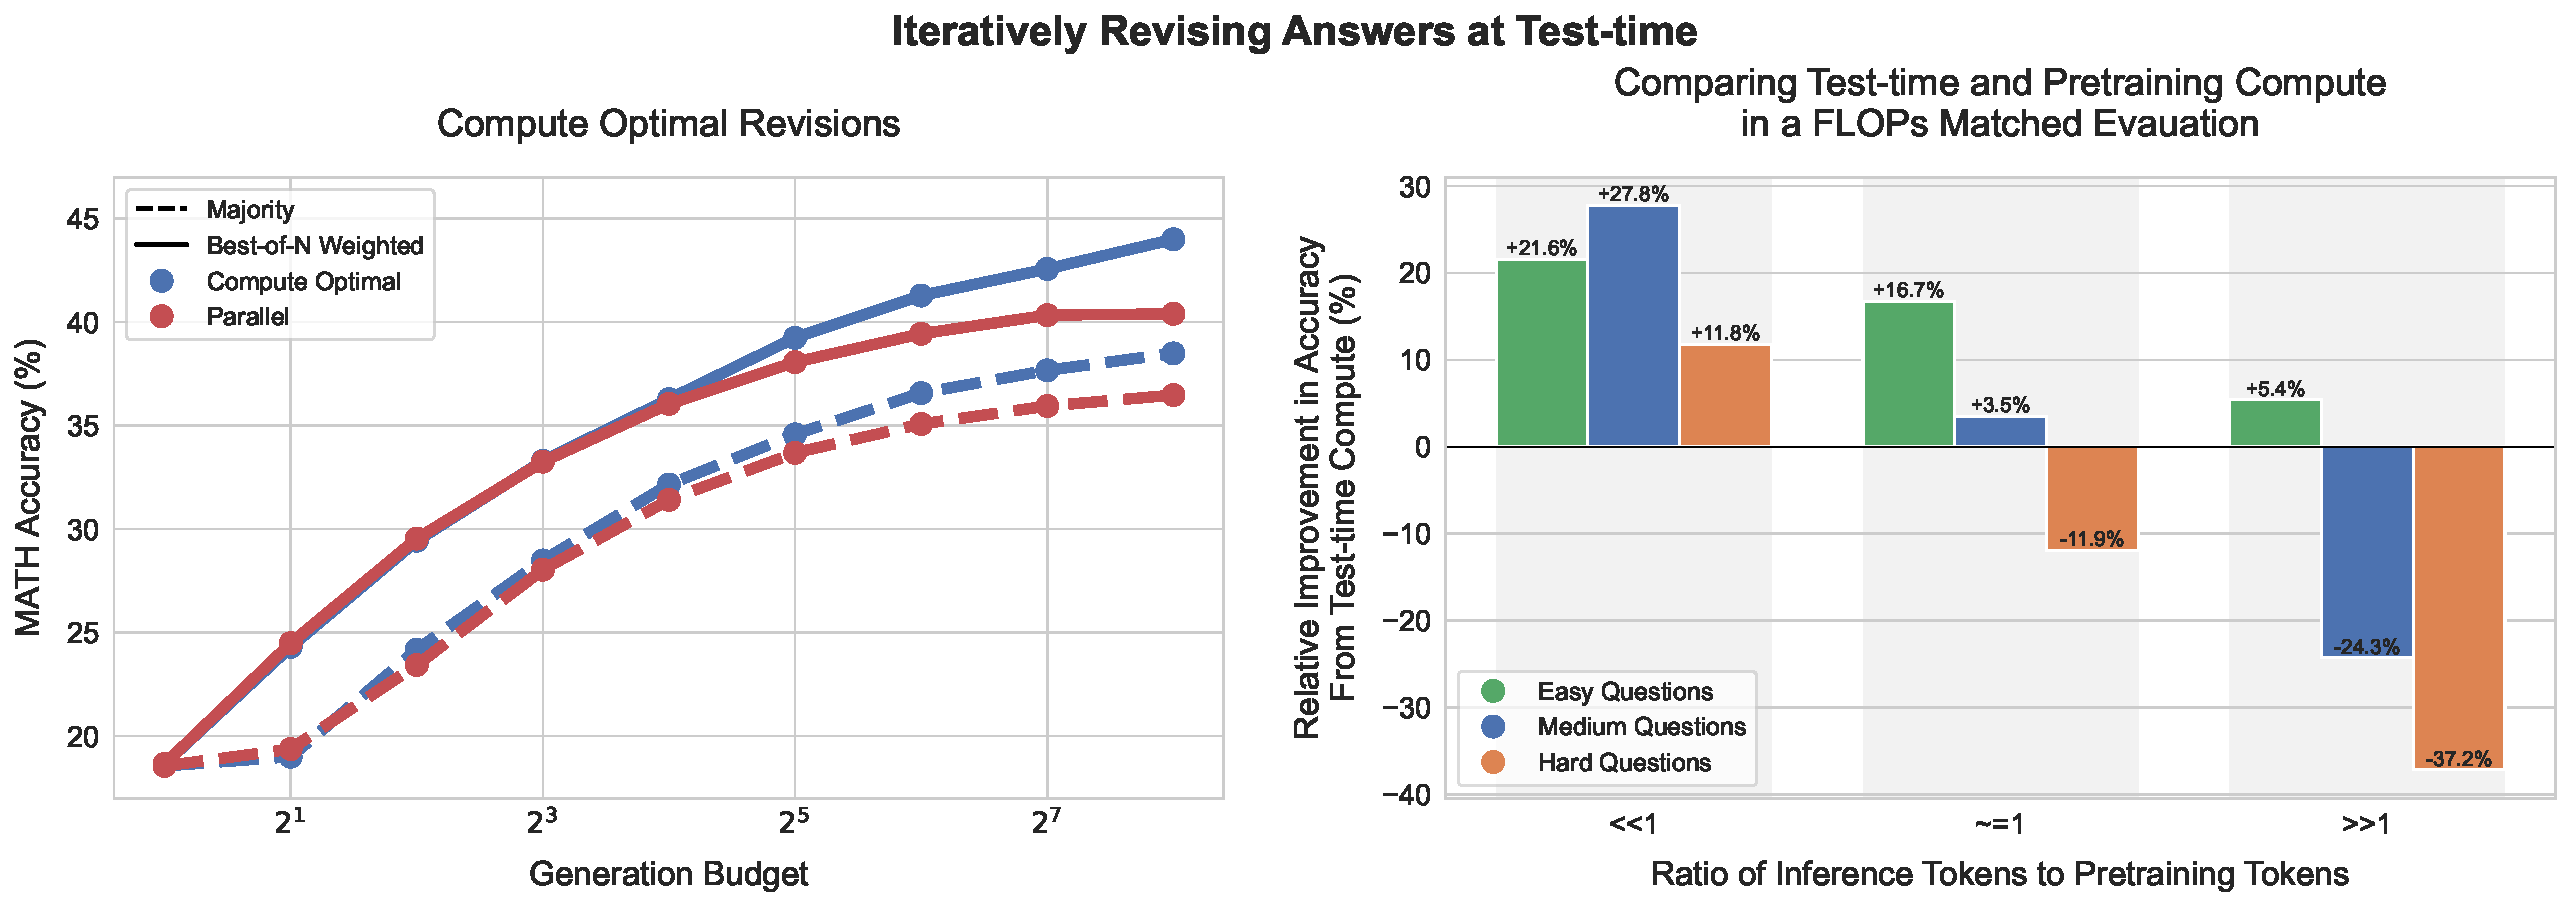
\includegraphics[width=.95\linewidth]{../papers/translations/testcompute/figures/revisions_fig1.pdf}\\
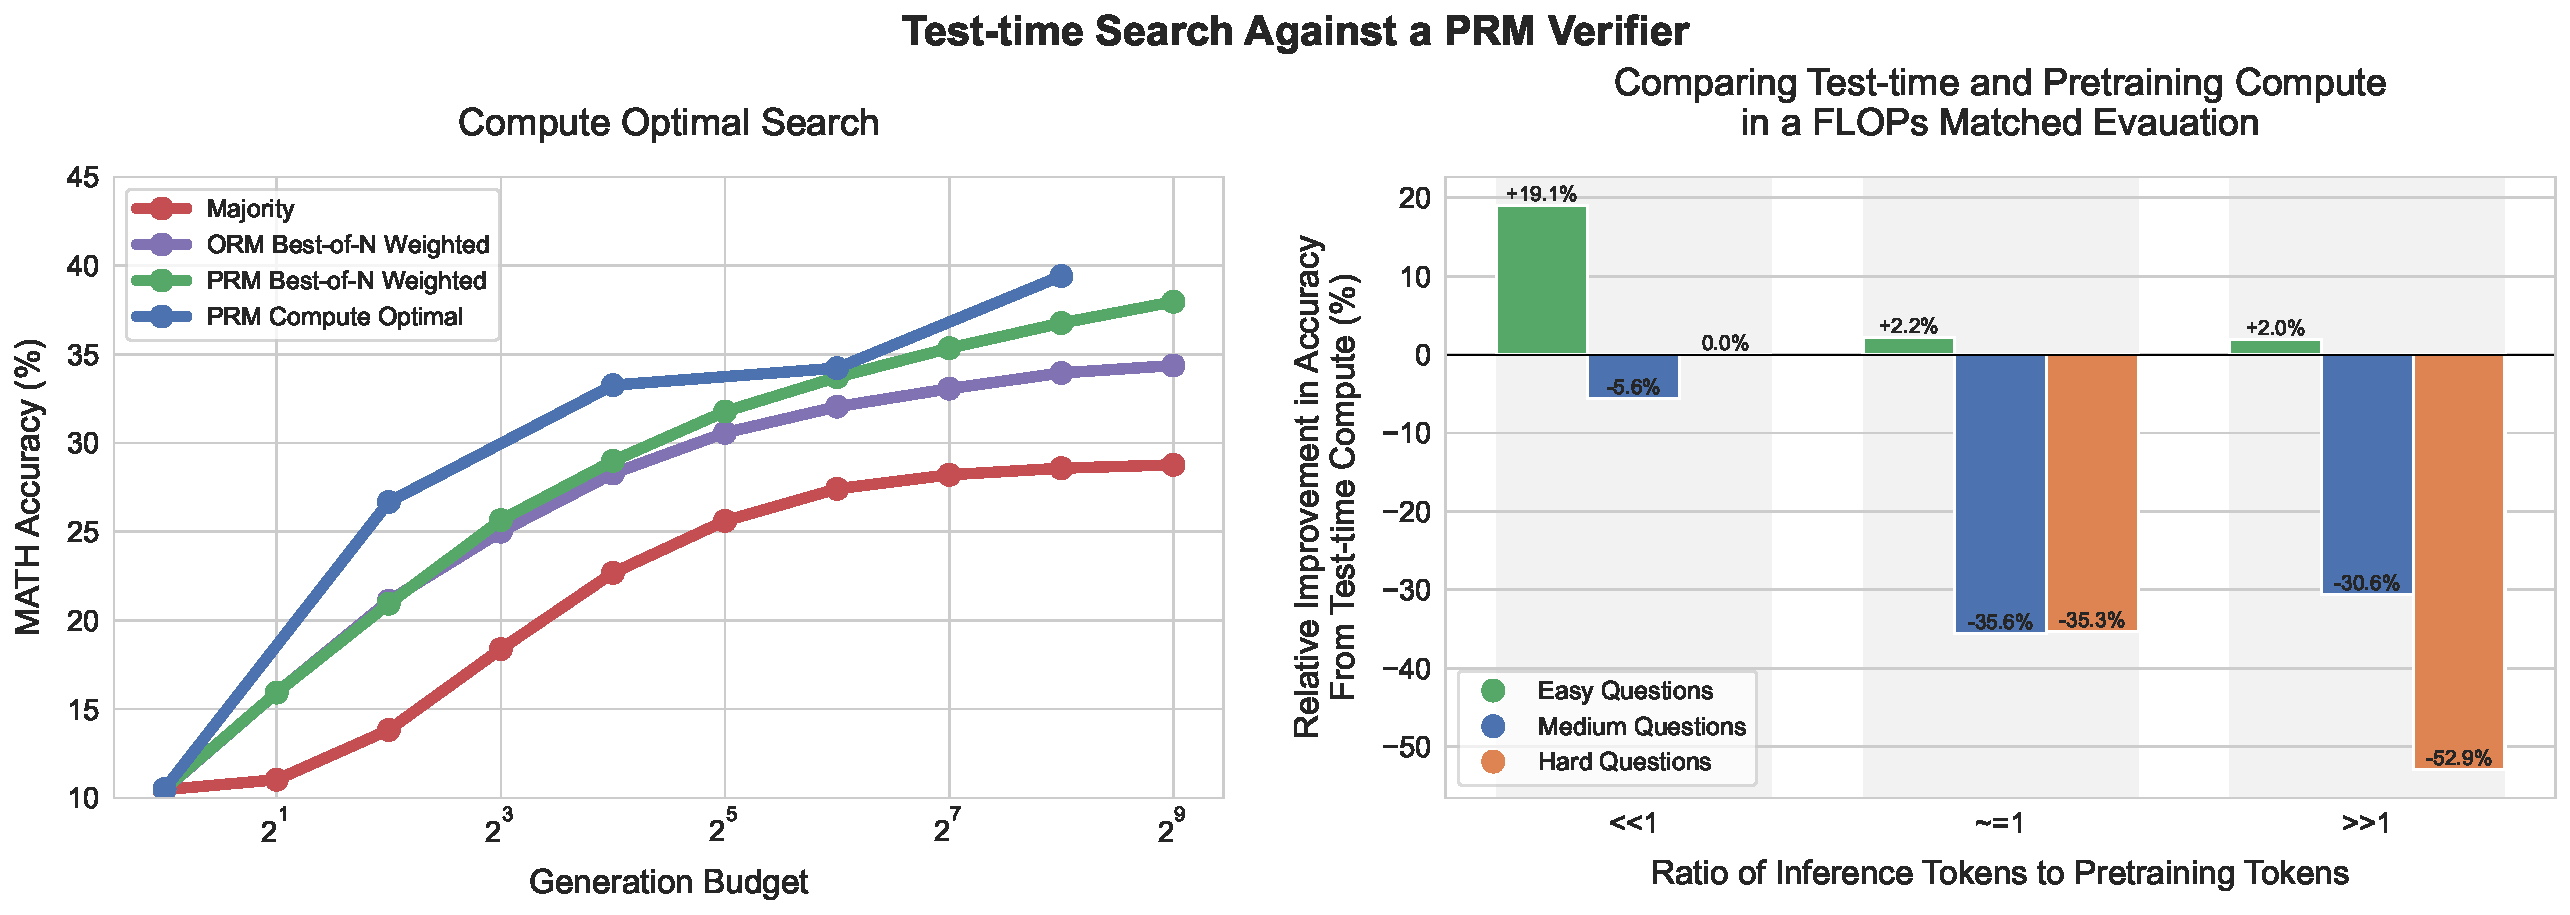
\includegraphics[width=.95\linewidth]{../papers/translations/testcompute/figures/prm_fig1.pdf}
\caption{原图 1: 我们的主要结果. \textbf{左: 迭代自我完善（即修订）与搜索的计算最优扩展. }左侧比较我们的 PaLM 2-S* 修订模型在修订设置（上）及 PRM 搜索设置（下）中的计算最优扩展策略与基线. 修订情况下, 标准 best-of-N（如“parallel”, 并行）与计算最优扩展的差距逐渐拉大, 使计算最优扩展能用 $1/4$ 的推理时计算超过 best-of-N. PRM 搜索情况下, 计算最优扩展早期也相对 best-of-N 有明显改进, 在某些点上几乎能以 $1/4$ 的计算超过 best-of-N. 详见原文第 5、6 节. \textbf{右: 推理时计算与模型参数扩展的比较. }比较 PaLM 2-S* 的计算最优推理时扩展和一个约大 $14$ 倍、没有额外推理时计算（如贪心采样）的预训练模型. 设两者都预训练 $X$ 个 token, 推理 $Y$ 个 token. 训练更大模型会同时倍增这两部分的 FLOPs 需求. 如果为较小模型增加推理时计算, 匹配较大模型的 FLOPs 需求, 准确性会如何? 修订（上）在 $Y\ll X$ 时, 推理时计算往往优于额外预训练. 但随着推理与预训练 token 的比例上升, 推理时计算仍在简单问题上更有利, 而在较难问题上预训练更有利. PRM 搜索（下）也有类似趋势. 详见原文第 7 节. }
\label{testcompute-fig:comparing_base_lms}
\end{figure}

以往关于推理时计算的研究结果并不一致. 一方面, 一些工作表明, 现有 LLM 能够使用推理时计算改善输出\cite{testcompute-bai2022constitutional,testcompute-madaan2023selfrefine,testcompute-du2023improving,testcompute-saunders2022selfcritiquing,testcompute-yao2023tree}; 另一方面, 其他工作表明, 这些方法在数学推理等更复杂任务上的有效性仍十分有限\cite{testcompute-huang2023large,testcompute-stechly2023gpt4,testcompute-valmeekam2023large}, 尽管推理问题通常需要的是对已有知识作出推断, 而非获取新知识. 这类相互冲突的发现说明, 有必要系统分析扩展推理时计算的不同方法. 

我们希望理解扩大推理时计算的收益. 可以说, 最简单、研究最充分的方法是 \emph{best-of-N} 采样: 从基础 LLM 中“并行”采样 $N$ 个输出, 再选择学习得到的验证器或奖励模型评分最高的一个\cite{testcompute-cobbe2021training,testcompute-lightman2023lets}. 不过, 这并非利用推理时计算改进 LLM 的唯一方法. 如本文所展示, 通过修改产生响应的\emph{提议分布}（例如要求基础模型“顺序”修订原始响应\cite{testcompute-qu2024recursive}）, 或者改变\emph{验证器}的用法（例如训练基于过程的稠密验证器\cite{testcompute-lightman2023lets,testcompute-wang2023mathshepherd}并依据它进行搜索）, 可以大幅改进推理时计算的扩展能力. 

为理解扩大推理时计算的收益, 我们在具有挑战性的 MATH 基准\cite{testcompute-hendrycks2021measuring}上开展实验, 使用经过专门微调的 PaLM-2 模型\cite{testcompute-anil2023palm}\footnote{为了让基础模型在 MATH 上获得修订与验证能力, 有必要开展针对这些能力的微调, 因为即使强大的专有 LLM 也缺乏这些能力\cite{testcompute-huang2023large,testcompute-sharma2024criticalevaluationaifeedback}. 但我们预期, 未来 LLM 会因规模增加以及纳入专门针对这些能力的额外数据而更擅长验证与修订\cite{testcompute-predictemergence,testcompute-blakeney2024doesdatasparkjoy,testcompute-llmcriticscatchbugs}. 因此, 为推进对推理时计算扩展的理解, 我们必须使用经过这些能力微调的模型. 不过, 我们预期未来模型会直接在预训练时获得这些能力, 从而不再需要针对能力的微调. }, 使其能够修订错误答案\cite{testcompute-qu2024recursive}（即改进提议分布; 第\ref{testcompute-sec:revisions}节）, 或用过程奖励模型（PRM）验证答案中各个步骤的正确性\cite{testcompute-lightman2023lets,testcompute-wang2023mathshepherd}（第\ref{testcompute-sec:search}节）. 对于这两种方法, 我们都发现, 某一推理时计算策略的有效性, 关键取决于具体问题的性质和所使用的基础 LLM. 例如, 对于基础 LLM 已经可以轻易产生合理响应的较简单问题, 让模型预测一系列 $N$ 次修订、迭代完善初始答案（即修改提议分布）, 可能比并行采样 $N$ 个独立响应更有效. 另一方面, 对于可能需要在许多不同高层解题途径中搜索的较难问题, 重新并行独立采样响应, 或依据过程奖励模型进行树搜索, 可能是更有效的推理时计算使用方式. 

这一发现说明, \textbf{扩展推理时计算需要部署自适应的“计算最优”策略}: 根据提示选择具体的推理时计算方法, 充分利用额外计算. 我们还表明, 从基础 LLM 角度定义的一种\emph{问题难度}（第\ref{testcompute-sec:setup}节）, 能够预测推理时计算的有效性, 从而让我们在给定提示时实际实现这种“计算最优”策略. 以这种方式合理分配推理时计算, 我们能大幅改进计算扩展, 在修订与搜索两种情况下, 都只用约 $1/4$ 的计算就超过 best-of-N 基线（第\ref{testcompute-sec:search}、\ref{testcompute-sec:revisions}节）. 

借助改进后的推理时计算扩展策略, 我们进一步希望理解, 推理时计算能在多大程度上有效替代额外预训练. 我们将增加推理时计算的较小模型, 与预训练一个\textbf{大 $14$ 倍的模型}进行 FLOPs 匹配比较. 我们发现, 在简单、中等问题上, 甚至在困难问题上（取决于预训练和推理工作负载的具体条件）, 额外推理时计算往往优于扩大预训练. 这表明, \textbf{在某些设置中, 用更少计算预训练较小模型, 然后通过推理时计算改善输出, 会更加有效}, 而非仅仅专注于扩大预训练. 不过, 在最具有挑战性的问题上, 我们观察到扩大推理时计算的收益很小. 相反, 这些问题更适合通过额外预训练计算取得进展, 说明现有推理时计算扩展方法可能无法与扩大预训练一比一互换. 总体而言, 这表明, 即使采用相当朴素的方法, 扩大推理时计算也已经可能优于扩大预训练, 而且随着推理时策略成熟, 还会有更多改进. 从长远看, 这暗示未来可能将较少 FLOPs 用于预训练, 而将更多 FLOPs 用于推理. 

\originalsection{2 推理时计算的统一视角: 提议器与验证器}
\paperlabel{2}{testcompute-sec:unifying_perspective}
我们首先统一使用推理时计算的各种方法, 再分析若干代表性方法. 我们将额外推理时计算视为: 在给定提示的条件下, 测试时\emph{自适应}修改模型预测的分布. 理想情况下, 这种计算应修改分布, 使输出优于直接从 LLM 本身朴素采样得到的输出. 一般有两种调节方式: \textbf{（1）输入层面}, 在给定提示中增添一组 token, 让 LLM 以它们为条件得到修改后的分布; \textbf{（2）输出层面}, 从标准语言模型中采样多个候选, 再对这些候选进行处理. 换言之, 可以修改 LLM 本身诱导的\textbf{提议分布}, 使其优于仅以提示为条件的朴素分布; 也可以使用事后的\textbf{验证器或评分器}修改输出. 这类似于马尔可夫链蒙特卡洛（MCMC）\cite{testcompute-andrieu2003introduction}: 结合一个简单提议分布和一个评分函数, 从复杂目标分布中采样. 通过改变输入 token 直接修改提议分布, 与使用验证器, 构成我们研究的两个独立维度. 

\textbf{修改提议分布. }改进提议分布的一种方法, 是通过 STaR 或 $\text{ReST}^{\text{EM}}$ 等受到强化学习启发的微调方法\cite{testcompute-zelikman2022star,testcompute-singh2024human}, 针对给定推理任务直接优化模型. 注意, 这些技术不使用额外输入 token, 而是专门微调模型, 诱导出改进后的提议分布. 相比之下, 自我批评等技术\cite{testcompute-bai2022constitutional,testcompute-madaan2023selfrefine,testcompute-du2023improving,testcompute-saunders2022selfcritiquing}, 通过要求模型迭代批评、修订自己的输出, 让模型在测试时自行改进提议分布. 由于仅靠提示现成模型, 无法有效地让它们在测试时进行修订, 我们专门微调模型, 使其在复杂推理设置下迭代修订答案. 为此, 我们采用在同策略数据上微调的方法, 用 best-of-N 引导模型响应的改进\cite{testcompute-qu2024recursive}. 

\textbf{优化验证器. }在提议分布与验证器的抽象中, 验证器负责从提议分布中聚合或选择最佳答案. 最典型的用法是 best-of-N 采样: 采样 $N$ 个完整解答, 再按验证器选择最佳解答\cite{testcompute-cobbe2021training}. 但还可以训练基于过程的验证器\cite{testcompute-lightman2023lets}, 即过程奖励模型（PRM）, 预测解答每个中间步骤的正确性, 而不只预测最终答案. 随后可用这些逐步预测, 在解答空间中进行树搜索, 与朴素 best-of-N 相比, 这可能提供更高效、更有效的依据验证器进行搜索的方式\cite{testcompute-yao2023tree,testcompute-feng2024alphazerolike,testcompute-chen2024alphamath}. 

\originalsection{3 如何最优地扩展推理时计算}
\paperlabel{3}{testcompute-sec:compute_optimal}
统一各种方法后, 我们现在希望理解: 对于给定提示, 如何\emph{最有效}地利用推理时计算改善语言模型表现. 具体要回答: 
\begin{remark}[问题设置]
给定一个提示, 以及解决问题时允许使用的推理时计算预算. 在上述抽象下, 推理时计算有不同用法. 每种方法的有效性可能随具体问题而变化. 对于给定提示, 如何确定\emph{最有效}的推理时计算用法? 与直接使用一个大得多的预训练模型相比, 这种做法会取得怎样的表现? 
\end{remark}
完善提议分布或依据验证器搜索时, 都有多种超参数可调整, 以决定如何分配推理时计算预算. 例如, 当提议分布来自专门为修订微调的模型, 而验证器是结果奖励模型（ORM）时, 可以将全部预算用于并行生成 $N$ 个独立样本, 再执行 best-of-N; 也可以用修订模型顺序采样 $N$ 次修订, 再用 ORM 从序列中选择最佳答案; 还可以在这两个极端之间折中. 直观上, “较简单”问题可能更受益于修订, 因为模型的初始样本更可能已经走在正确方向上, 只是需要进一步完善. 相比之下, 具有挑战性的问题可能需要更多探索不同的高层解题策略, 因此在这种设置下, 多次独立并行采样可能更合适. 

对于验证器, 还可以选择不同搜索算法（如束搜索、前瞻搜索、best-of-N）; 它们的性质可能随验证器与提议分布的质量而不同. 与简单得多的 best-of-N 或多数投票基线相比, 更复杂的搜索过程可能在更难问题上更有用. 

\subsection*{3.1 推理时计算最优扩展策略}
\paperlabel{3.1}{testcompute-sec:compute-optimal-strategy}
因此, 总的来说, 我们希望为给定问题选择推理时计算预算的\emph{最优}分配. 对于任意给定的推理时计算方法（如本文的修订、依据验证器的搜索, 或其他地方的各种方法）, 我们将\textbf{“推理时计算最优扩展策略”}定义为: 在测试时, 对给定提示, 选择某一推理时策略的超参数, 使表现收益最大化. 形式上, 令 $\operatorname{Target}(\theta,N,q)$ 为模型在提示 $q$、推理时计算超参数 $\theta$ 和计算预算 $N$ 下诱导的自然语言输出 token 分布. 我们希望选择使给定问题的目标分布准确率最大化的超参数 $\theta$, 即
\begin{equation}
\theta^{*}_{q,a^*(q)}(N)=\operatorname{argmax}_{\theta}
\left(\mathbb E_{y\sim\operatorname{Target}(\theta,N,q)}
\left[\mathbf 1_{y=y^*(q)}\right]\right).
\label{testcompute-eq:test_time_compute_optimal}
\end{equation}
其中 $y^*(q)$ 为 $q$ 的真实正确响应, $\theta^{*}_{q,y^*(q)}(N)$ 为问题 $q$ 在计算预算 $N$ 下的推理时计算最优扩展策略. 
\begin{remark}
译者注: 原文式（1）左端下标写作 $a^*(q)$, 紧随其后的定义则写作 $y^*(q)$. 这里保留这一记号差异; 指示函数的字形由原来的黑板体 $1$ 调整为粗体 $1$, 含义相同. 
\end{remark}

\subsection*{3.2 为计算最优扩展估计问题难度}
\paperlabel{3.2}{testcompute-sec:estimating-difficulty}
为了有效分析第\ref{testcompute-sec:unifying_perspective}节中不同机制（如提议分布与验证器）的推理时扩展性质, 我们以给定提示的一个统计量为依据, 为最优策略 $\theta^{*}_{q,y^*(q)}(N)$ 给出近似. 这一统计量估计提示的一种\emph{难度}, 计算最优策略则定义为提示难度的函数. 尽管这只是式\eqref{testcompute-eq:test_time_compute_optimal}问题的近似解, 我们发现, 相比以临时拼凑方式或均匀采样方式分配推理时计算的基线, 它仍能显著提高表现. 

难度估计将问题分为五个难度等级. 对于给定推理时计算预算, 可以利用这一离散难度类别, 在验证集上估计 $\theta^{*}_{q,y^*(q)}(N)$, 再将计算最优策略应用于测试集. 具体而言, 我们为每个难度分箱独立选择表现最佳的推理时计算策略. 由此, 在设计计算最优策略时, 问题难度充当了问题的充分统计量. 

\textbf{定义问题难度. }遵循 Lightman 等人\cite{testcompute-lightman2023lets}的方法, 我们将难度定义为给定基础 LLM 的函数. 具体而言, 对测试集每题, 利用 $2048$ 个样本估计模型的 pass@1, 将这些数值分为五个分位组, 分别对应递增的难度等级. 我们发现, 与 MATH 数据集中人工标注的难度分箱相比, 这种模型特定难度分箱更能预测推理时计算的有效性. 

不过, 按上述方式评估难度, 假定可以访问真实正确性检查函数这一预言机. 部署时, 只有不知道答案的测试提示, 当然没有这种访问权限. 为使方法在实践中可行, 我们因此也考虑不用真实标签来评估难度. 具体而言, 对每题同一组 $2048$ 个样本, 我们根据学习得到的验证器的预测正确率（而非真实答案的正确性检查）评估难度. 我们称这种设置为\textbf{模型预测难度}, 依赖真实正确性的设置为\textbf{预言机难度}. 

模型预测难度虽然不需要知道真实标签, 但这种难度估计仍带来额外推理计算成本. 不过, 这种一次性的推理成本可以计入实际执行推理时策略的成本中（例如使用验证器时, 可以用同一推理计算同时进行搜索）. 更一般地, 这类似强化学习的探索与利用权衡: 在实际部署条件下, 必须平衡评估难度和执行最计算最优方法所花的计算. 这是未来研究的重要方向（见第\ref{testcompute-sec:discussion}节）. 我们的实验主要为简便而未计入这项成本, 因为目标是给出一批最初的结果, 说明通过有效分配推理时计算, \emph{实际上可能做到什么}. 

为避免在计算难度分箱和选择计算最优策略时使用同一测试集而造成混淆, 我们在测试集每个难度分箱内进行二折交叉验证. 在一折上按表现选择最佳策略, 再用它评估另一折; 随后交换两折, 最后平均两次测试结果. 

\originalsection{4 实验设置}
\paperlabel{4}{testcompute-sec:setup}
我们先概述使用多种验证器设计与提议分布进行分析的实验设置, 再在后续各节给出分析结果. 

\textbf{数据集. }我们预期, 当模型已具备回答问题所需的全部基本“知识”, 主要挑战只是从这些知识作出（复杂）推断时, 推理时计算最有帮助. 因此, 我们聚焦 MATH 基准\cite{testcompute-hendrycks2021measuring}; 它由高中竞赛水平、具有不同难度的数学问题构成. 所有实验均采用 Lightman 等人\cite{testcompute-lightman2023lets}使用的数据划分: $12\mathrm{k}$ 个训练问题、$500$ 个测试问题. 

\textbf{模型. }我们使用 PaLM 2-S*\cite{testcompute-anil2023palm}（Codey）基础模型进行分析. 我们认为该模型能代表许多当代 LLM 的能力, 因此研究发现很可能迁移到类似模型. 尤其是, 该模型在 MATH 上表现并非微不足道, 同时尚未饱和, 所以我们预期它能提供良好的实验平台. 

\originalsection{5 通过验证器扩展推理时计算}
\paperlabel{5}{testcompute-sec:search}
本节分析如何通过优化验证器, 尽可能有效地扩展推理时计算. 为此, 我们研究使用过程验证器（PRM）进行测试时搜索的不同方法, 并分析这些方法的推理时计算扩展性质. 

\subsection*{5.1 训练适于搜索的验证器}
\paperlabel{5.1}{testcompute-sec:training-verifiers}
\textbf{PRM 训练. }最初的 PRM 训练\cite{testcompute-uesato2022solving,testcompute-lightman2023lets}使用人工众包标注. 尽管 Lightman 等人\cite{testcompute-lightman2023lets}发布了 PRM 训练数据（PRM800k 数据集）, 我们发现, 这些数据对我们而言基本无效. 即使采用 best-of-N 采样这样的朴素策略, 也很容易利用在此数据集上训练的 PRM 的漏洞. 我们推测, 这可能源于该数据集中 GPT-4 生成样本与我们的 PaLM 2 模型之间的分布偏移. 我们没有继续采用为 PaLM 2 收集众包 PRM 标签这一昂贵过程, 而是使用 Wang 等人\cite{testcompute-wang2023mathshepherd}的方法: 从解答的每个步骤开始运行蒙特卡洛续采样, 估计逐步正确性, 无需人工标签即可监督 PRM. 因此, 我们的 PRM 逐步预测对应基础模型采样策略的未来累计奖励价值估计, 与近期工作\cite{testcompute-wang2023mathshepherd,testcompute-setlur2024rl}类似. 我们也与 ORM 基线比较（附录\ref{testcompute-app:comparing_prm_orm}）, 但发现 PRM 始终优于 ORM. 因此本节所有搜索实验都使用 PRM. 训练细节见附录\ref{testcompute-app:prm_training}. 

\textbf{答案聚合. }测试时, 可以用过程验证器为从基础模型采样得到的一组解答逐步评分. 用 PRM 选择 best-of-N 答案时, 需要一个函数, 聚合每个答案的各步骤得分, 以确定正确答案的最佳候选. 我们先将每个答案的逐步得分聚合为完整答案的最终得分（步骤内聚合）, 再跨答案聚合, 确定最佳答案（答案间聚合）. 具体如下: 
\begin{itemize}
\item \textbf{步骤内聚合. }我们不取逐步得分的乘积或最小值\cite{testcompute-wang2023mathshepherd,testcompute-lightman2023lets}, 而以 PRM 在最后一步的预测作为整个答案的得分. 我们发现, 这在研究的全部聚合方法中表现最好（见附录\ref{testcompute-app:comparing_prm_agg}）. 
\item \textbf{答案间聚合. }遵循 Li 等人\cite{testcompute-li2023making}, 使用“加权 best-of-N”选择, 而非标准 best-of-N. 加权 best-of-N 对最终答案相同的所有解答的验证器正确性分数求和, 即将其边缘化, 再选择总和最大的最终答案. 
\end{itemize}

\subsection*{5.2 依据 PRM 的搜索方法}
\paperlabel{5.2}{testcompute-sec:search-methods}
\begin{figure}[htbp]
\centering
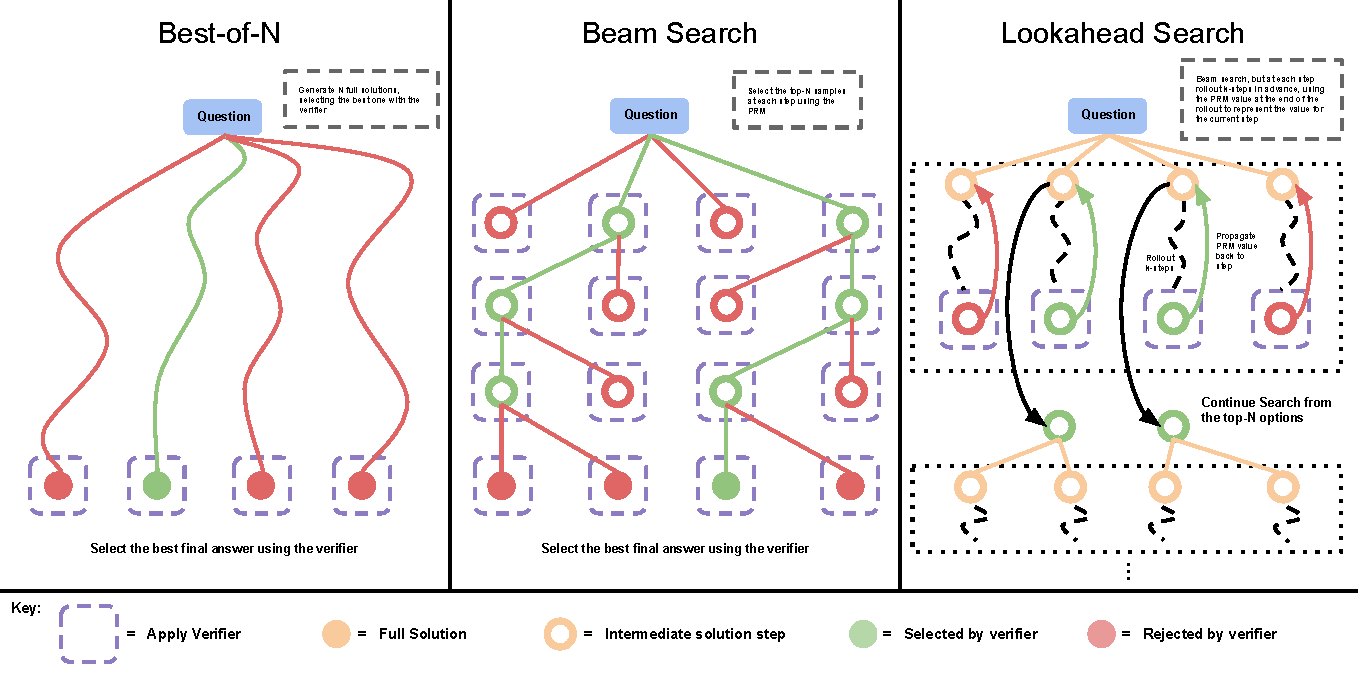
\includegraphics[width=.97\linewidth]{../papers/translations/testcompute/figures/Search_Figure-2.pdf}
\caption{原图 2: 不同 PRM 搜索方法的比较. \textbf{左: }best-of-N 采样 $N$ 个完整答案, 再按 PRM 的最终得分选择最佳答案. \textbf{中: }束搜索每步采样 $N$ 个候选, 再按 PRM 选取前 $M$ 个继续搜索. \textbf{右: }前瞻搜索扩展束搜索的每一步, 在评估保留哪些步骤继续搜索时, 使用 $k$ 步前瞻, 因此需要更多计算. }
\label{testcompute-fig:search_methods}
\end{figure}
我们通过搜索方法在测试时优化 PRM, 研究三种从少样本提示的基础 LLM（见附录\ref{testcompute-app:prompting}）采样输出的搜索方法, 示意见图\ref{testcompute-fig:search_methods}. 

\textbf{加权 best-of-N. }从基础 LLM 独立采样 $N$ 个答案, 再按 PRM 对最终答案的判断选择最佳答案. 

\textbf{束搜索. }束搜索通过搜索 PRM 的逐步预测来优化 PRM. 我们的实现类似 BFS-V\cite{testcompute-yao2023tree,testcompute-feng2024alphazerolike}. 具体而言, 考虑固定的束数量 $N$ 和束宽 $M$, 随后运行: 
\begin{enumerate}
\item 为解答的第一步采样 $N$ 个初始预测. 
\item 按 PRM 预测的逐步未来累计奖励估计, 为生成的步骤评分（本设置中奖励稀疏, 因此这也对应从前缀出发的总奖励）. 
\item 仅保留得分最高的前 $N/M$ 个步骤. 
\item 从每个候选出发, 为下一步采样 $M$ 个提议, 再次得到总计 $(N/M)\times M$ 个候选前缀. 重复步骤 2--4. 
\end{enumerate}
算法运行到解答结束, 或达到最大束扩展轮数（我们为 $40$ 轮）. 搜索结束时得到 $N$ 个最终答案候选, 再应用上面的加权 best-of-N 选择, 给出最终预测. 
\begin{remark}
译者注: 原图 2 的图注使用“选取前 $M$ 个”的表述, 正文算法则明确保留 $N/M$ 个、每个再扩展 $M$ 个. 译文分别保留两处原文, 不替作者统一参数定义. 
\end{remark}

\textbf{前瞻搜索. }前瞻搜索改变束搜索评估单个步骤的方式. 它用前瞻续采样提高搜索过程中每一步 PRM 价值估计的准确性. 具体而言, 在束搜索每一步, 它不直接用当前步骤的 PRM 得分选取最佳候选, 而是进行一次模拟, 向前最多续采样 $k$ 步; 若到达解答末尾, 则提前停止. 为最小化模拟续采样的方差, 使用温度 $0$. 然后用这次续采样结束位置的 PRM 预测, 为束搜索当前步骤评分. 换言之, 束搜索可以视为 $k=0$ 的前瞻搜索特例. 若 PRM 准确, 增大 $k$ 应能提高逐步价值估计准确性, 代价是额外计算. 还要注意, 这种前瞻搜索是 MCTS\cite{testcompute-suttonrlbook}的特例; 因为 PRM 已训练完成且被冻结, 所以删去了 MCTS 中为促进探索而设计的随机成分. 这些随机成分主要有助于学习价值函数（我们已通过 PRM 学得）, 但测试时希望利用而非探索, 它们就不那么有用. 因此, 前瞻搜索基本能代表测试时应用 MCTS 风格方法的方式. 

\begin{figure}[htbp]
\centering
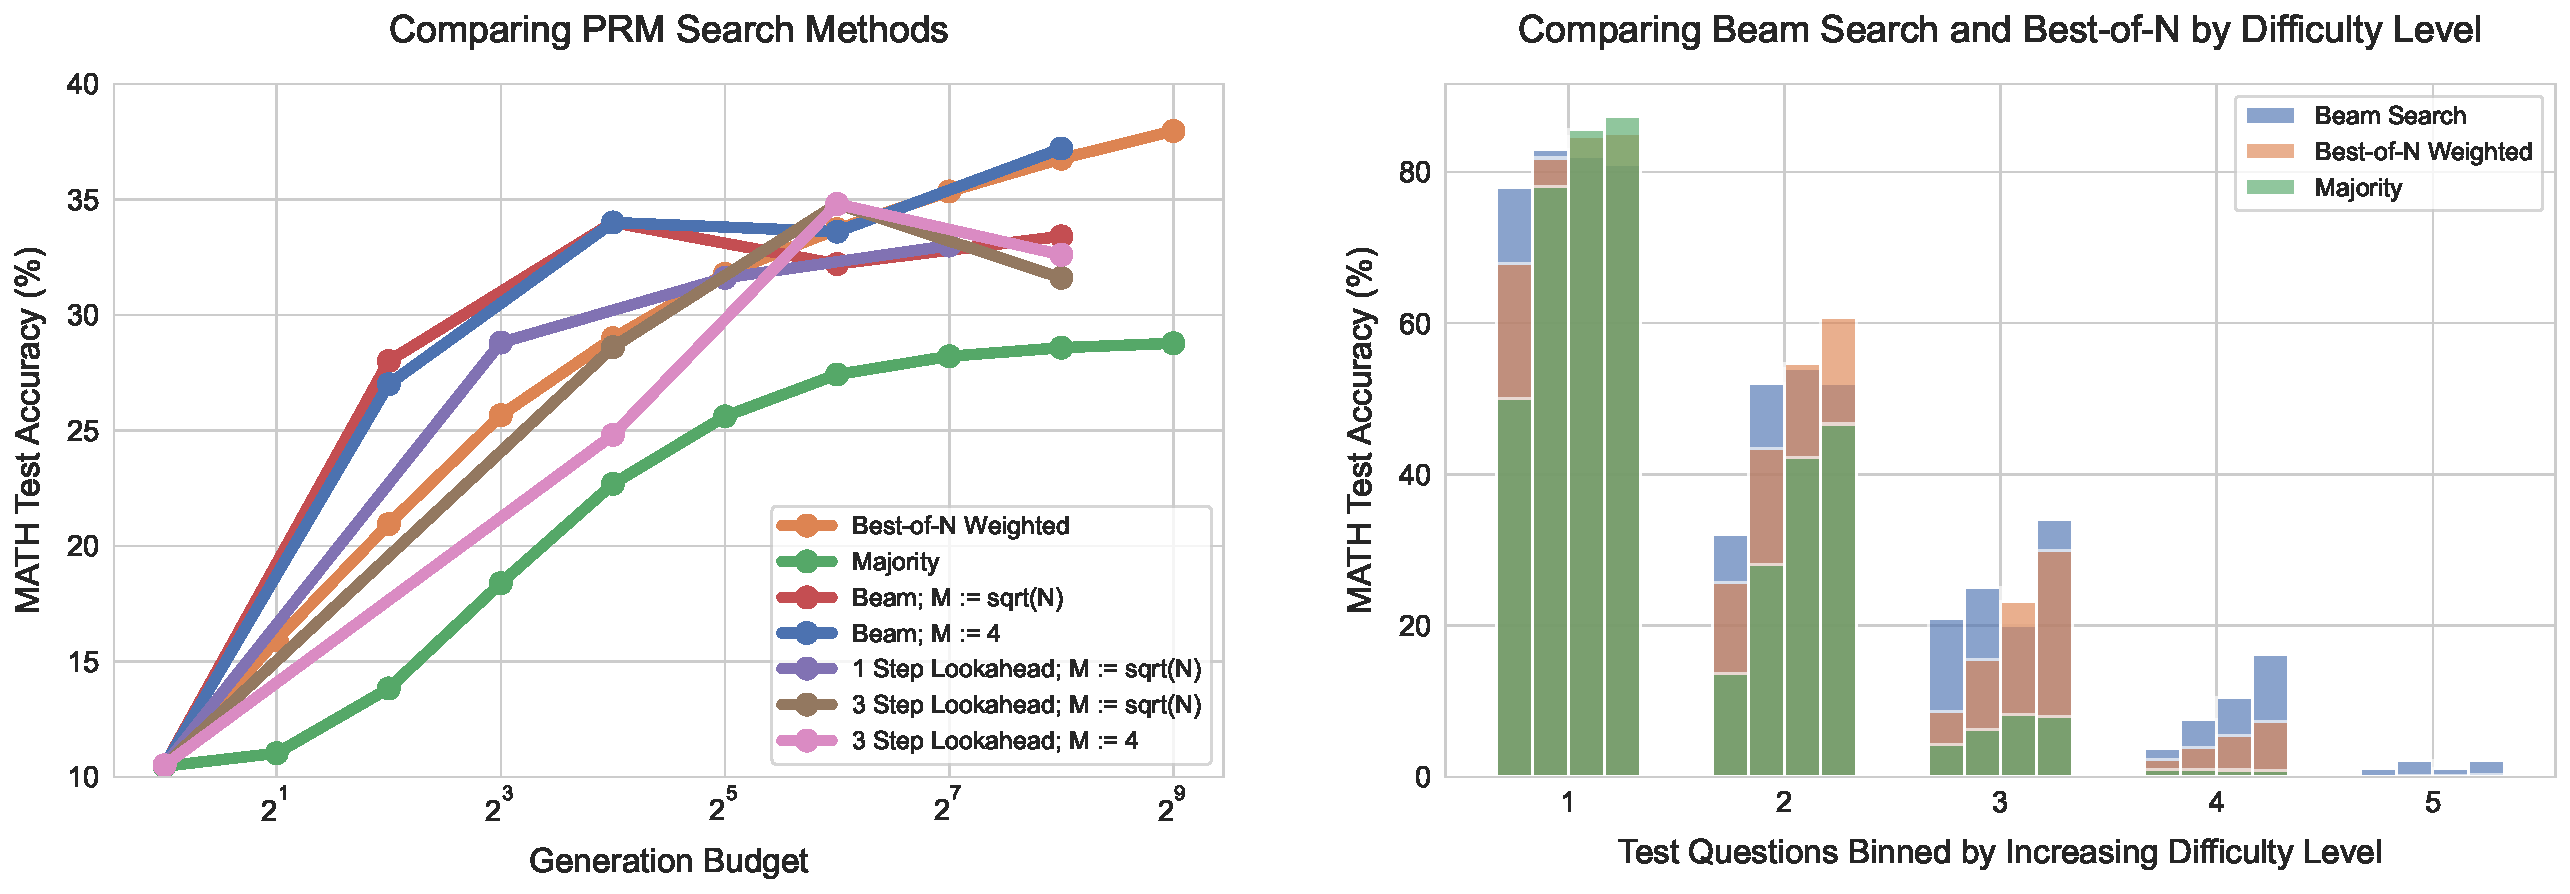
\includegraphics[width=.99\linewidth]{../papers/translations/testcompute/figures/search_comparing_and_bins3.pdf}
\caption{原图 3. \textbf{左: 依据 PRM 验证器搜索的不同方法. }生成预算低时, 束搜索最好; 但进一步扩大预算后, 改进逐渐减少, 表现落到 best-of-N 基线之下. 在同一生成预算下, 前瞻搜索通常不如其他方法. \textbf{右: 按难度分箱比较束搜索与 best-of-N. }每个难度分箱中的四根柱表示递增的推理时计算预算（$4$、$16$、$64$、$256$ 次生成）. 在较简单问题（分箱 1、2）上, 较高预算下束搜索显示出过度优化迹象, best-of-N 则没有. 在中等难度问题（分箱 3、4）上, 束搜索持续优于 best-of-N. }
\label{testcompute-fig:comparing_search_and_beam_difficulty}
\end{figure}

\subsection*{5.3 分析结果: 使用验证器搜索的推理时扩展}
\paperlabel{5.3}{testcompute-sec:search-analysis}
现在比较各搜索算法, 并为搜索方法确定一种依赖提示难度的计算最优扩展策略. 

\textbf{比较搜索算法. }首先扫描各种搜索设置. 除标准 best-of-N 外, 我们扫描区分不同树搜索方法的两个主要参数: 束宽 $M$ 与前瞻步数 $k$. 虽然无法广泛扫描每种配置, 我们在最大预算 $256$ 下扫描以下设置: 
\begin{enumerate}
\item 束宽为 $\sqrt N$ 的束搜索, 其中 $N$ 为生成预算. 
\item 固定束宽为 $4$ 的束搜索. 
\item 对上述设置 1、2 都应用 $k=3$ 的前瞻搜索. 
\item 对设置 1 应用 $k=1$ 的前瞻搜索. 
\end{enumerate}
为按生成预算公平比较搜索方法, 我们建立各方法成本的估计协议. 一次生成指从基础 LLM 采样一个答案. 束搜索与 best-of-N 的生成预算分别对应束数量和 $N$. 前瞻搜索则使用额外计算: 每个搜索步骤再向前采样 $k$ 个额外步骤. 因此, 我们将其成本定义为 $N\times(k+1)$ 个样本. 

\textbf{结果. }图\ref{testcompute-fig:comparing_search_and_beam_difficulty}左侧显示, 生成预算较小时, 束搜索显著优于 best-of-N. 但扩大预算后, 这些改进大幅减弱, 束搜索常常低于 best-of-N 基线. 我们还看到, 同样生成预算下, 前瞻搜索通常低于其他方法, 可能因为模拟前瞻续采样引入额外计算. 搜索收益递减, 可能是由于利用了 PRM 预测的漏洞. 例如, 在一些实例中（如图\ref{testcompute-fig:prm_ex6}）, 搜索使模型在解答末尾生成信息量很低的重复步骤. 其他情况下, 过度优化搜索会得到仅含 1--2 步的过短解答. 这解释了为何最强大的搜索方法（前瞻搜索）表现下降最多. 附录\ref{testcompute-app:prm_example_outputs}给出若干搜索得到的实例. 

\textbf{搜索改善了哪些问题? }为理解如何计算最优地扩展搜索方法, 我们进行难度分箱分析, 具体比较束搜索（$M=4$）与 best-of-N. 图\ref{testcompute-fig:comparing_search_and_beam_difficulty}右侧显示, 虽然在高生成预算下两者总体表现相似, 按难度分箱评估却呈现迥异趋势. 简单问题（等级 1、2）上, 两种方法中更强的优化器——束搜索——随着生成预算增加而降低表现, 暗示其利用了 PRM 信号的漏洞. 较难问题（等级 3、4）上, 束搜索始终超过 best-of-N. 最难问题（等级 5）上, 没有方法取得多少有意义的进展. 

这些发现符合直觉: 简单问题上, 验证器的正确性判断可能大多准确. 因此, 进一步用束搜索优化, 只会进一步放大验证器学到的虚假特征, 使表现恶化. 较难问题上, 基础模型起初采样到正确答案的概率低得多, 搜索因此能引导模型更经常地产生正确答案. 

\begin{figure}[htbp]
\centering
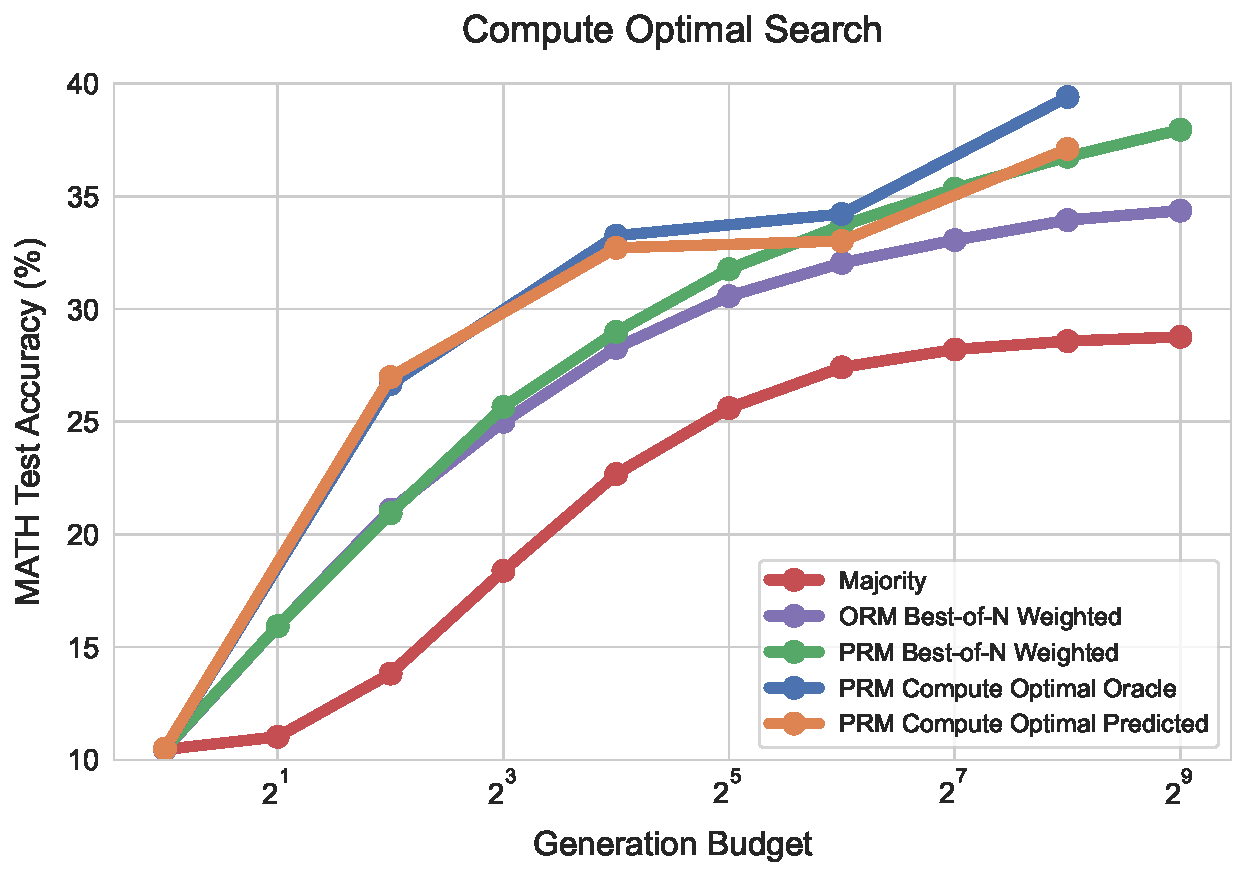
\includegraphics[width=.68\linewidth]{../papers/translations/testcompute/figures/compute_optimal_search_v4.pdf}
\caption{原图 4: PRM 搜索中计算最优推理时计算分配与基线的比较. 按问题难度扩展推理时计算, 几乎能以少至 $1/4$ 的推理时计算超过 PRM best-of-N（如 $16$ 次对 $64$ 次生成）. “compute-optimal oracle”表示使用由真实正确性信息得到的预言机难度分箱; “compute-optimal predicted”表示使用 PRM 的预测产生难度分箱. 两种分箱的曲线基本重合. }
\label{testcompute-fig:compute_optimal_search}
\end{figure}
\textbf{计算最优搜索. }根据以上结果, 问题难度显然是预测给定计算预算下最优搜索策略的有用统计量. 最佳策略也可能随这一统计量发生剧烈变化. 因此, 图\ref{testcompute-fig:compute_optimal_search}用每个难度等级中表现最佳的搜索策略, 展示“计算最优”扩展趋势. 低生成预算下, 使用预言机难度与预测难度, \textbf{计算最优扩展都几乎能以少至 $1/4$ 的推理时计算超过 best-of-N}（如 $16$ 次对 $64$ 次生成）. 高预算下, 预测难度的部分收益减弱, 但使用预言机分箱时, 最优扩展仍持续改善. 这表明, 搜索期间自适应分配推理时计算可能带来表现收益. 

\begin{remark}[验证器计算最优扩展的要点]
我们发现, 任意给定验证器搜索方法的有效性, 都关键取决于计算预算与当前问题. 具体而言, 束搜索在较难问题与较低计算预算下更有效; best-of-N 在较简单问题与较高预算下更有效. 此外, 针对给定难度与推理时计算预算选择最佳搜索设置, 几乎能用少至 $1/4$ 的推理时计算超过 best-of-N. 
\end{remark}

\originalsection{6 完善提议分布}
\paperlabel{6}{testcompute-sec:revisions}
此前研究了依据验证器搜索的推理时计算扩展性质; 现在转向修改提议分布的扩展性质（第\ref{testcompute-sec:unifying_perspective}节）. 具体而言, 我们使模型能够迭代修订自己的答案, 在测试时动态改进自身分布. 简单提示现有 LLM 纠正自身错误, 在推理问题上通常基本不能改善表现\cite{testcompute-huang2023large}. 因此, 我们基于 Qu 等人\cite{testcompute-qu2024recursive}的方案, 加入适合本设置的修改, 微调语言模型, 使其能够迭代修订自己的答案. 先介绍如何训练和使用模型, 让它们以自己先前的解题尝试为条件, 顺序完善自身提议分布, 再分析修订模型的推理时扩展性质. 

\begin{figure}[htbp]
\centering
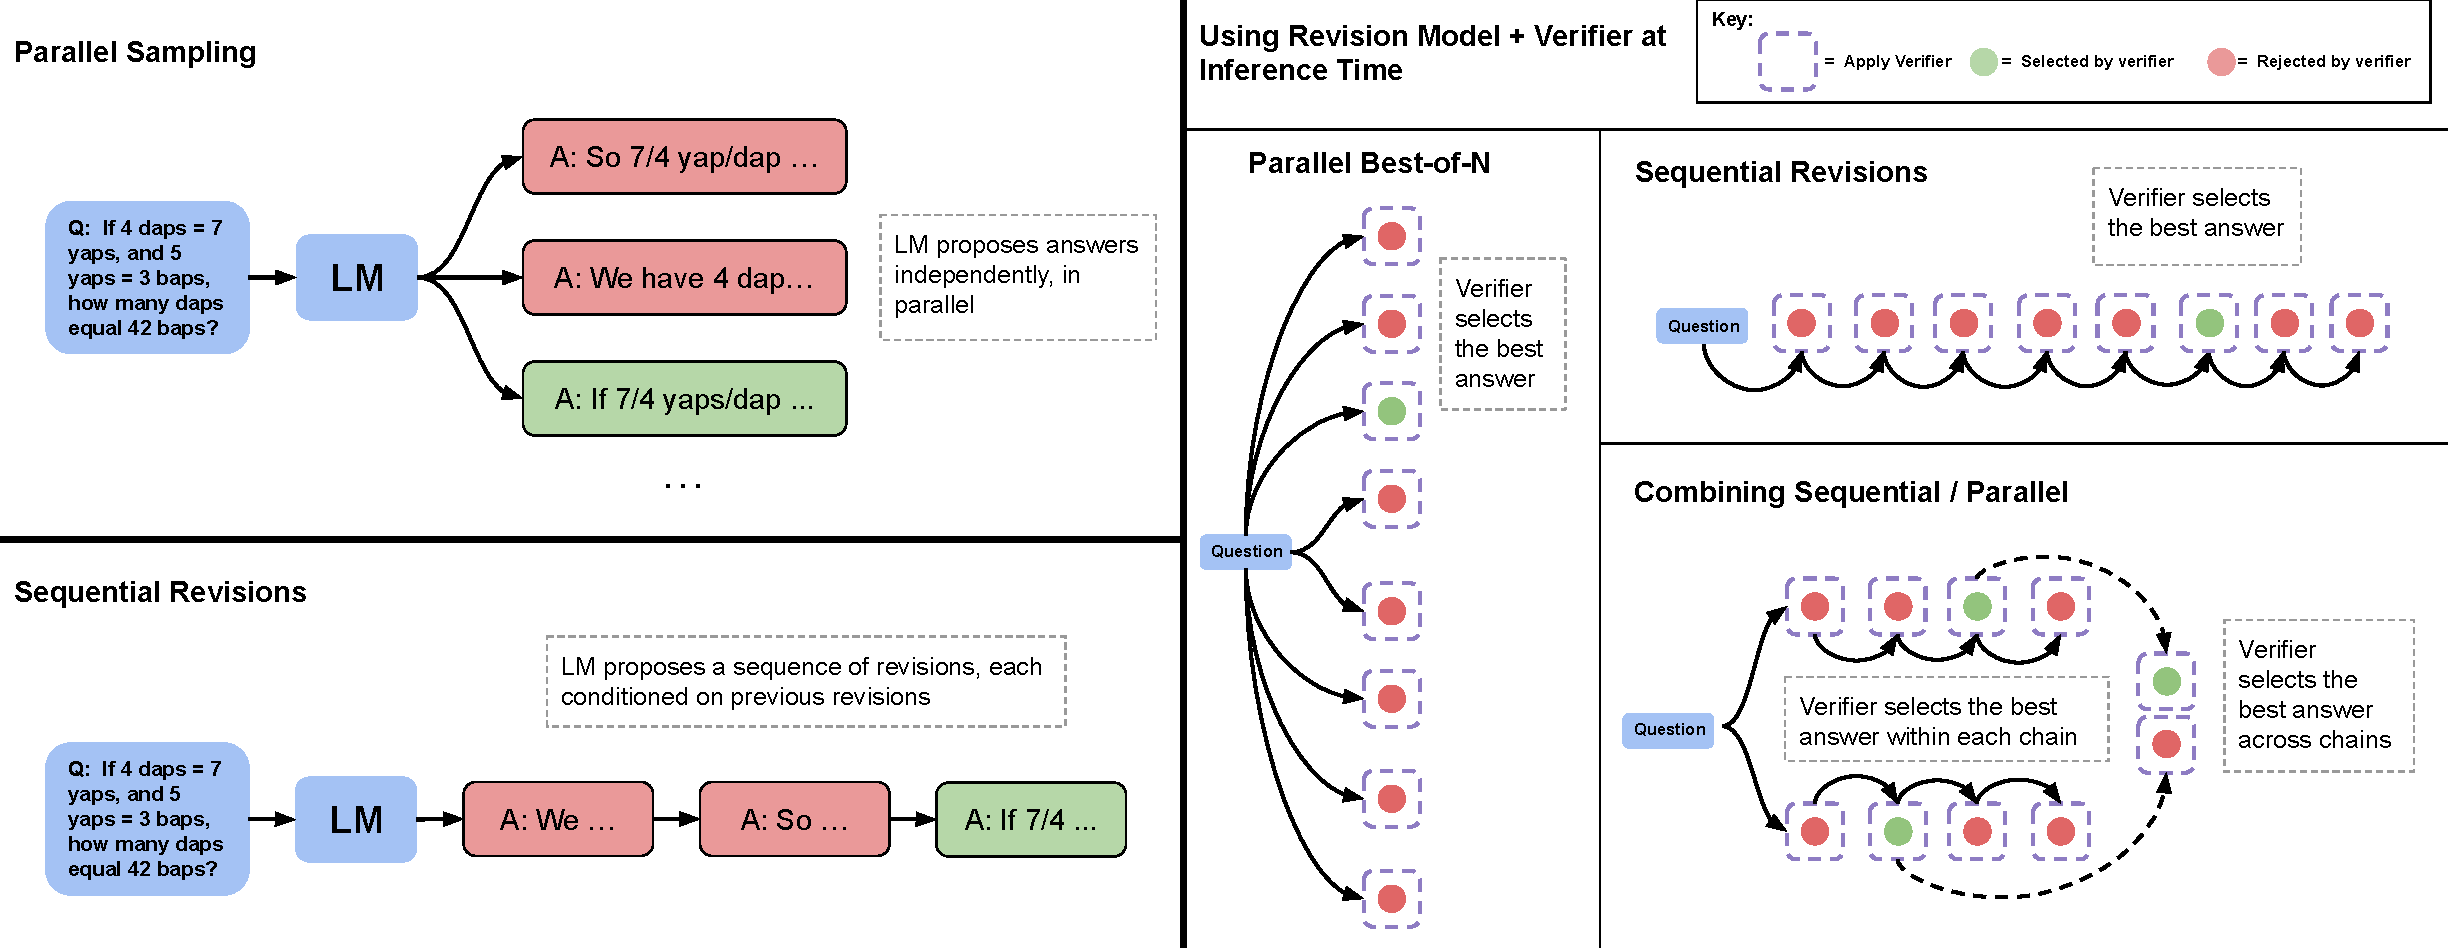
\includegraphics[width=.99\linewidth]{../papers/translations/testcompute/figures/Revisions_descriptive_fig.pdf}
\caption{原图 5: 并行采样（如 best-of-N）与顺序修订. \textbf{左: }并行采样独立并行生成 $N$ 个答案; 顺序修订则以先前尝试为条件, 依次生成答案. \textbf{右: }两种情况都可使用验证器确定 best-of-N 答案（如使用加权 best-of-N）. 也可将部分预算用于并行、部分用于顺序, 结合两种策略. 这时先用验证器选择各顺序链内的最佳答案, 再跨链选择最佳答案. }
\label{testcompute-fig:how_revisions_works}
\end{figure}

\subsection*{6.1 设置: 训练和使用修订模型}
\paperlabel{6.1}{testcompute-sec:revision_setup}
我们的修订模型微调过程类似 Qu 等人\cite{testcompute-qu2024recursive}, 但引入若干关键差异. 微调需要由一系列错误答案、最后接一个正确答案构成的轨迹, 再对它们进行监督微调（SFT）. 理想情况下, 正确答案应与上下文中的错误答案\emph{相关}, 从而有效教会模型\emph{隐式}识别上下文示例中的错误, 再通过编辑来纠正, 而非完全忽视上下文示例, 从头再试. 

\textbf{生成修订数据. }Qu 等人\cite{testcompute-qu2024recursive}获取多轮续采样的同策略方法已被证明有效, 但多轮续采样的计算成本使它在我们的基础设施中并不完全可行. 因此, 我们在较高温度下\emph{并行}采样 $64$ 个响应, 再从独立样本事后构造多轮续采样. 具体而言, 遵循文献\cite{testcompute-anonymousrevisions}的方案, 将每个正确答案与该样本集合中的一系列错误答案配对, 以错误答案为上下文, 构造多轮微调数据. 上下文最多含四个错误答案; 具体个数从 0--4 的类别均匀分布中随机采样. 用字符编辑距离度量, 优先选择与最终正确答案相关的错误答案（见附录\ref{testcompute-app:revision_finetune}）. 注意, token 编辑距离并非相关性的完美度量, 但我们发现, 与随机配对互不相关的错误和正确响应相比, 这一启发式足以使错误上下文答案与正确目标答案相关, 从而帮助训练有意义的修订模型. 
\begin{remark}
译者注: 本段前面称“字符编辑距离”, 后面称“token 编辑距离”; 附录 H 明确写 character-level. 这里保留正文原有表述差异. 
\end{remark}

\textbf{推理时使用修订. }给定微调后的修订模型, 测试时可从中采样修订序列. 虽然训练时上下文最多只有四个先前答案, 但只保留最近四个修订响应即可采样更长的链. 图\ref{testcompute-fig:revision_model_results}左侧显示, 随着链变长, 每步 pass@1 逐渐提高, 说明我们能够有效教会模型从上下文先前答案的错误中学习. 

\begin{figure}[htbp]
\centering
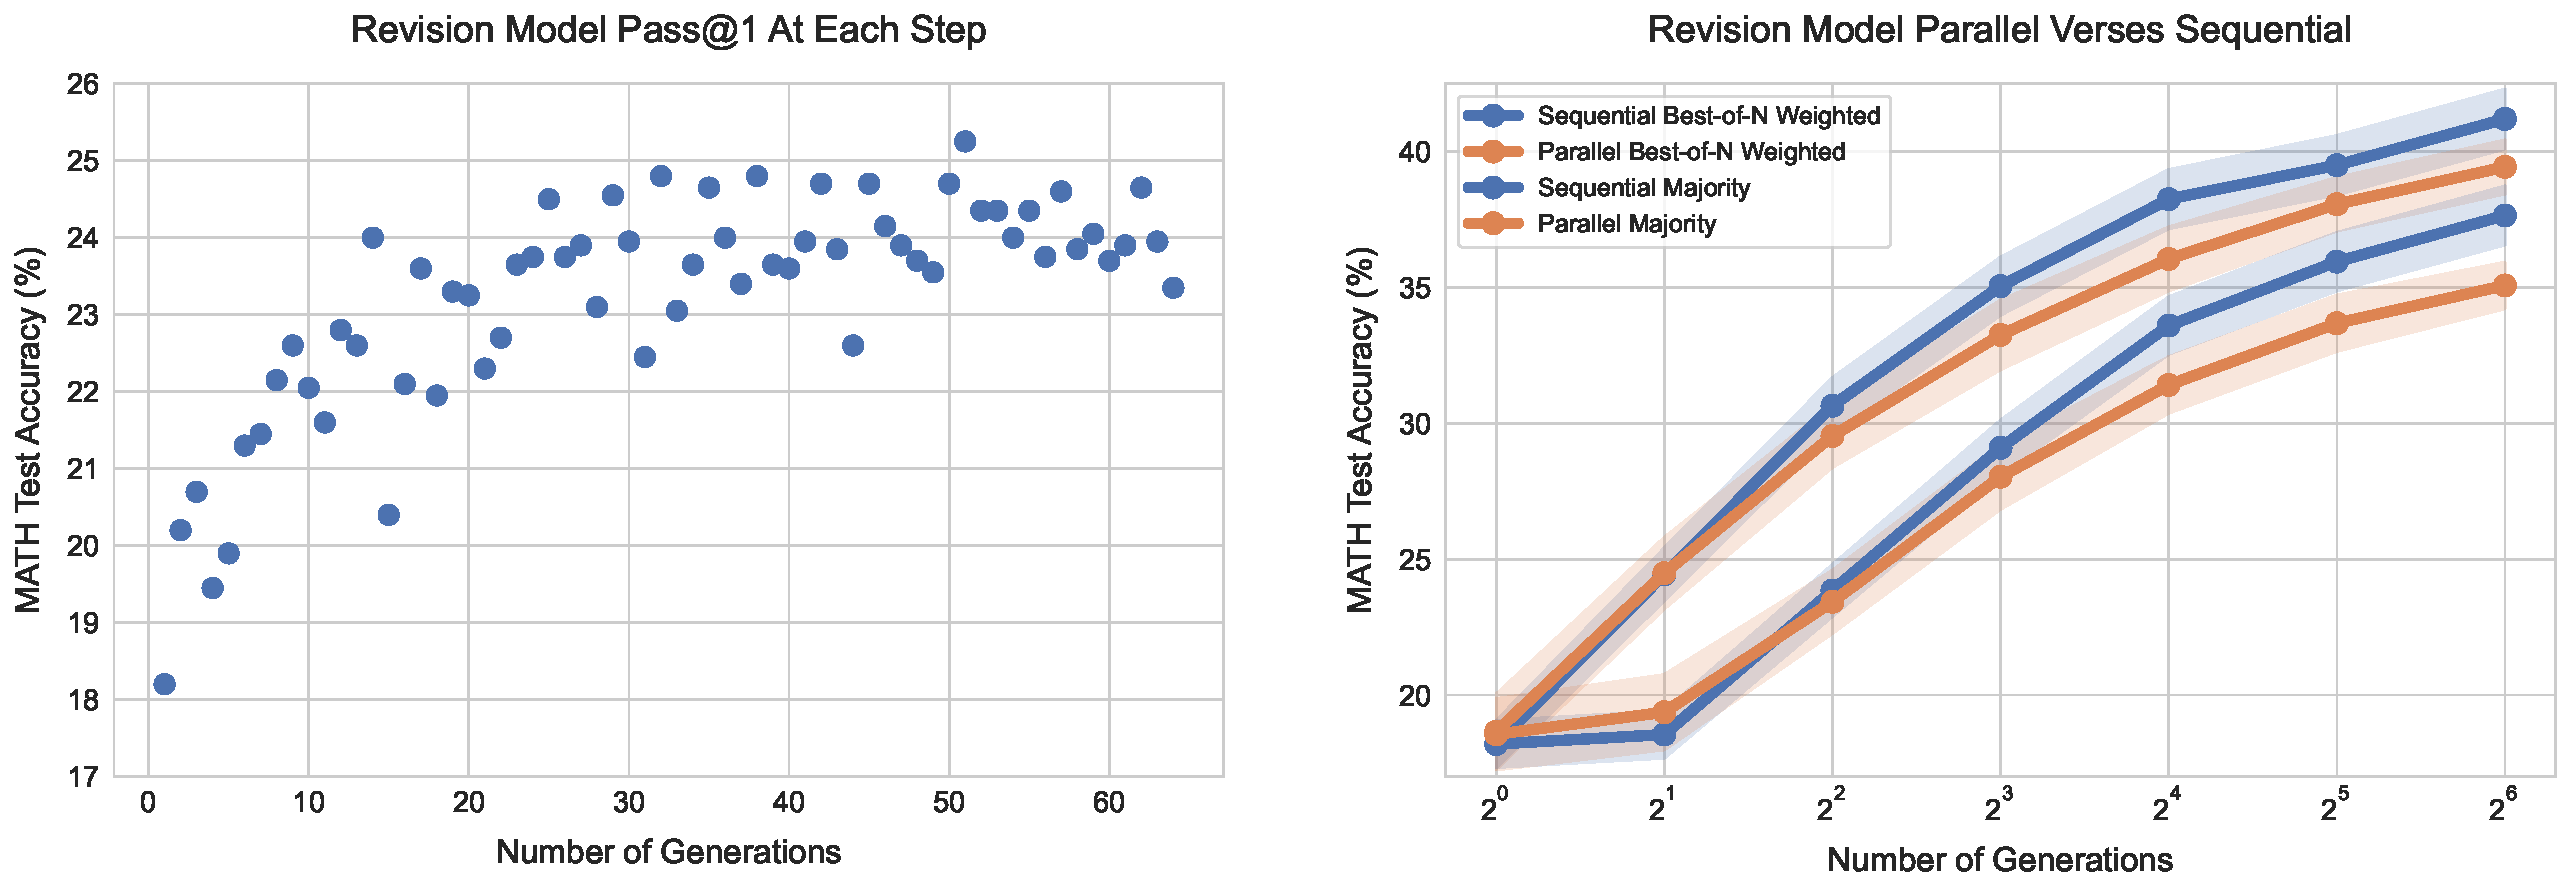
\includegraphics[width=.99\linewidth]{../papers/translations/testcompute/figures/pass1_and_comparing_seq_parallel.pdf}
\caption{原图 6. \textbf{左: 修订模型每个修订步骤的 pass@1. }每次修订后 pass@1 逐渐提高, 甚至在超过训练所用四个修订步骤后仍继续改善. 对测试集每题生成四条长度 $64$ 的修订轨迹, 平均表现来估计每步 pass@1. \textbf{右: 修订模型的顺序与并行采样. }比较并行生成 $N$ 个初始答案与顺序生成 $N$ 次修订. 无论用验证器还是多数投票选择答案, 顺序生成都略胜于并行生成. }
\label{testcompute-fig:revision_model_results}
\end{figure}
不过, 推理时存在分布偏移: 训练仅使用上下文答案全部错误的序列, 测试时则可能采到正确答案并将其纳入上下文. 这时下一步修订可能意外地将正确答案改错. 我们确实发现, 与 Qu 等人\cite{testcompute-qu2024recursive}相似, 朴素使用修订模型时, 约 $38\%$ 的正确答案会重新变成错误答案. 因此, 我们采用顺序多数投票或基于验证器的选择机制, 从修订序列中选出最正确的答案（见图\ref{testcompute-fig:how_revisions_works}）, 产生最佳答案. 

\textbf{比较. }为了检验用修订修改提议分布的有效性, 我们公平比较顺序采样 $N$ 次修订与并行采样 $N$ 次解题尝试的表现. 图\ref{testcompute-fig:revision_model_results}右侧显示, 无论是验证器还是多数投票选择机制, 顺序采样解答都优于并行采样. 

\begin{figure}[htbp]
\centering
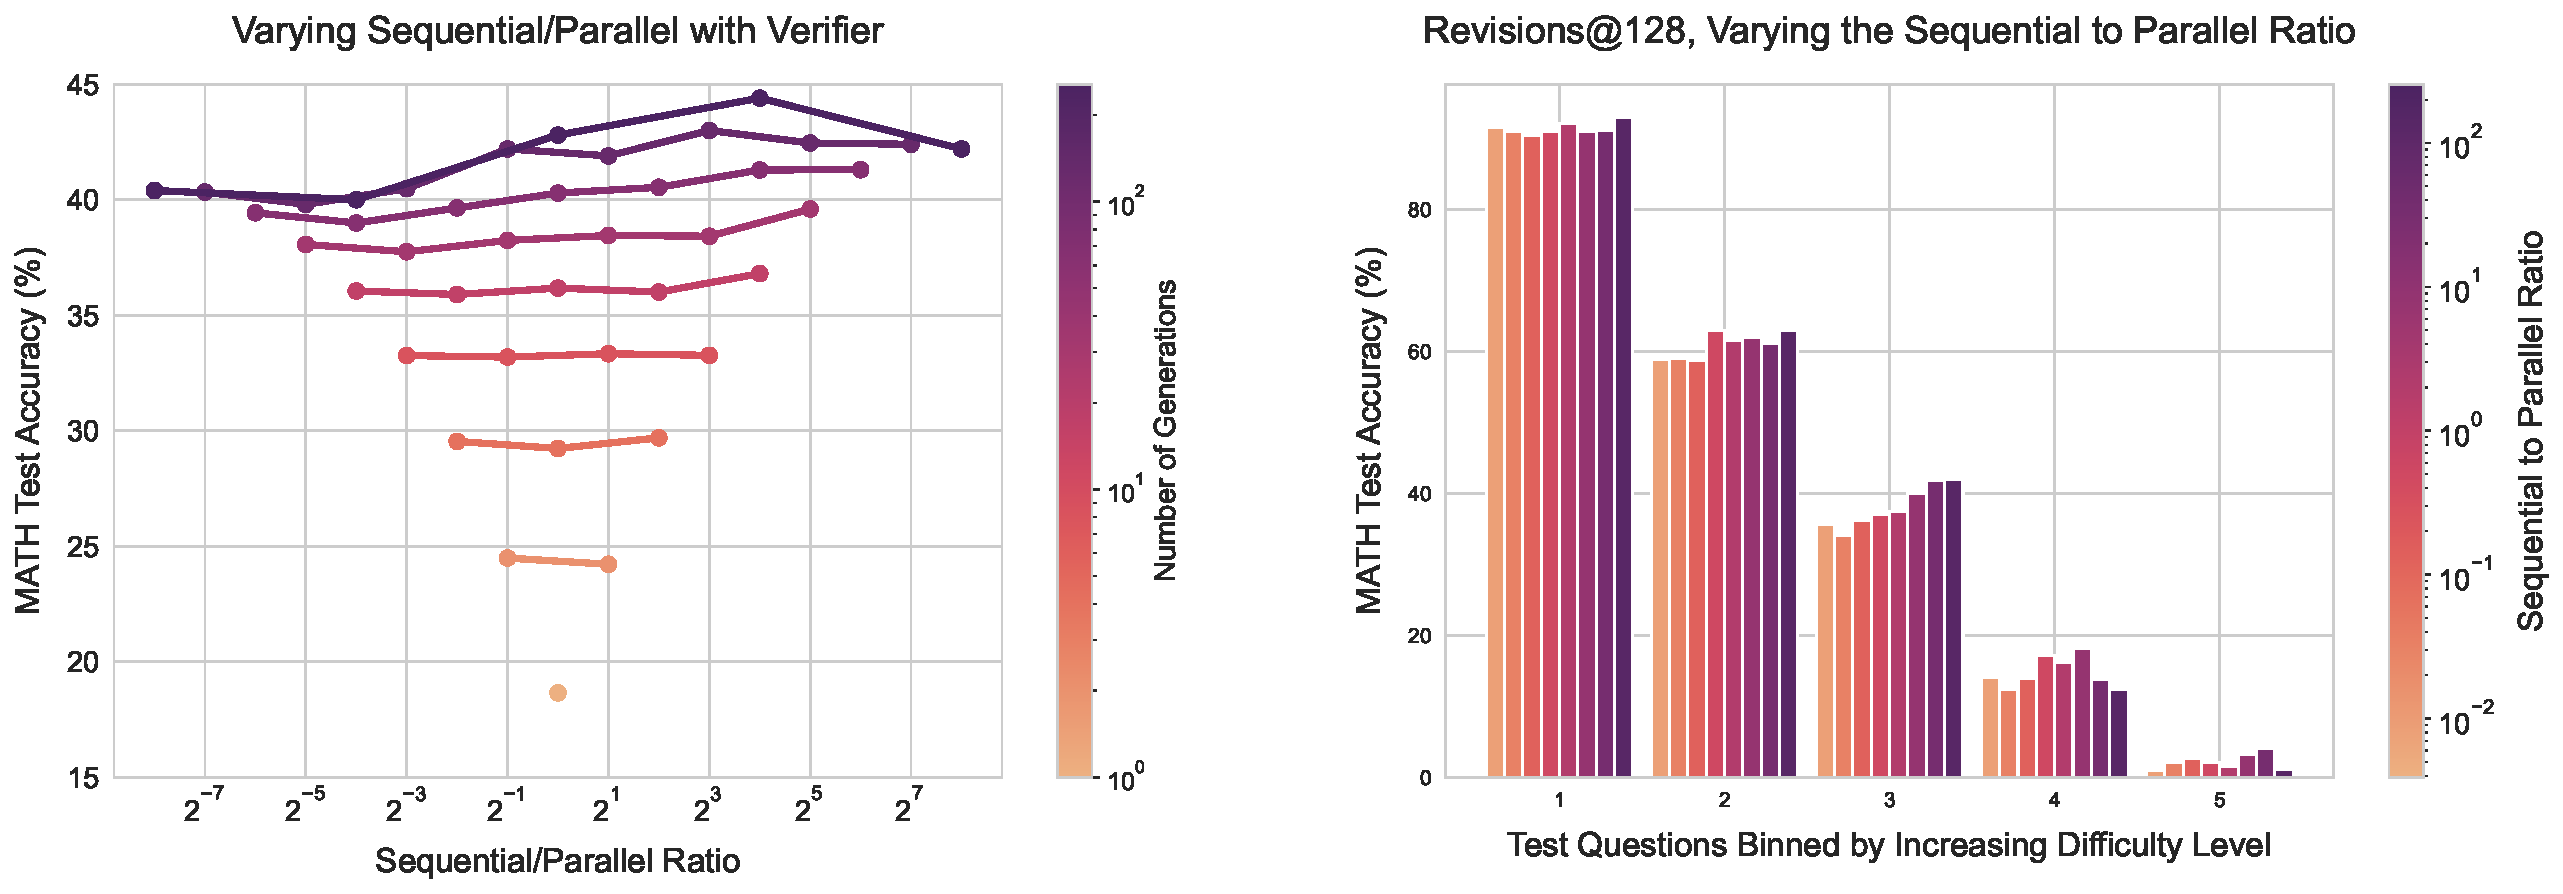
\includegraphics[width=.99\linewidth]{../papers/translations/testcompute/figures/revisions_varing_ratio_and_with_difficulty.pdf}
\caption{原图 7. \textbf{左: 改变生成预算用于顺序修订与并行样本的比例. }每条线对应固定生成预算, 比例变化; 用验证器选择答案. 虽然更多顺序修订通常优于更多并行计算, 但较高预算下存在平衡两个极端的理想比例. \textbf{右: 预算 $128$ 下, 各难度分箱的顺序与并行比例变化. }验证器选择时, 简单问题在全部顺序计算下最好; 困难问题存在理想的顺序与并行推理时计算比例. }
\label{testcompute-fig:iso_revisions}
\end{figure}

\subsection*{6.2 分析结果: 通过修订扩展推理时计算}
\paperlabel{6.2}{testcompute-sec:revision-analysis}
此前看到, 顺序提议答案优于并行提议. 但可以预期, 顺序与并行采样具有不同性质. 并行采样更像全局搜索, 原则上能够覆盖许多完全不同的解题途径, 例如不同候选可能采用完全不同的高层方法. 顺序采样则可能更像局部完善过程, 修订那些已经大体走在正确方向上的响应. 由于这些收益互补, 应在两个极端之间取得平衡: 将部分预算用于并行采样（如 $\sqrt N$）, 其余用于顺序修订（如 $\sqrt N$）. 现在我们将展示顺序与并行采样间存在计算最优比例, 并按给定提示的难度理解两者各自优缺点. 

\textbf{权衡顺序与并行推理时计算. }为理解如何最优分配顺序与并行计算, 我们扫描多个比例. 图\ref{testcompute-fig:iso_revisions}左侧显示, 给定生成预算下, \textbf{确实存在使准确率最大的理想顺序与并行比例}. 图\ref{testcompute-fig:iso_revisions}右侧还显示, 这一理想比例随问题难度而变化. 特别是, 简单问题更受益于顺序修订, 而困难问题最好在顺序与并行计算间折中. 这支持如下假设: 顺序修订（改变提议分布）与并行采样（用验证器搜索）是扩展推理时计算的两个互补维度, 按提示分别使用可能更有效. 模型生成实例见附录\ref{testcompute-app:revision_example_outputs}, 额外结果见附录\ref{testcompute-app:additional_revision}. 

\begin{figure}[htbp]
\centering
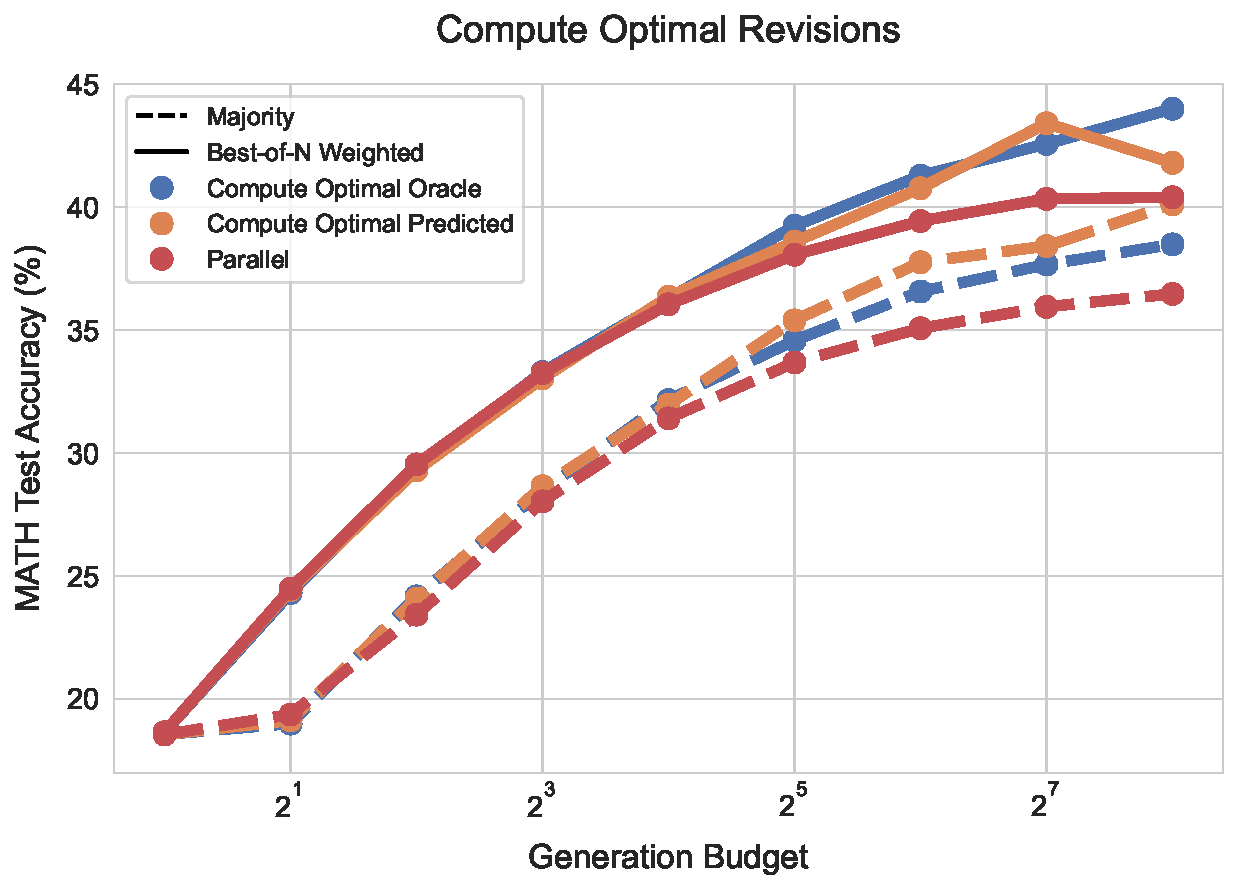
\includegraphics[width=.68\linewidth]{../papers/translations/testcompute/figures/compute_optimal_revisions_v4.pdf}
\caption{原图 8: 修订模型中计算最优推理时计算分配与并行计算基线的比较. 根据难度最优扩展推理时计算, 能以少至 $1/4$ 的推理时计算超过 best-of-N（如 $64$ 个对 $256$ 个样本）. “compute-optimal oracle”使用真实正确性信息得到的预言机难度分箱; “compute optimal predicted”使用 PRM 预测得到的模型预测难度分箱. }
\label{testcompute-fig:compute_optimal_revisions}
\end{figure}
\textbf{计算最优修订. }既然顺序与并行采样的有效性取决于难度, 就可以为每个难度分箱选择理想比例. 图\ref{testcompute-fig:compute_optimal_revisions}同时给出预言机难度与预测难度下的计算最优扩展结果. 两种情况下, 通过修订改进提议分布, 都能显著改善推理时计算扩展. 特别是, 较高生成预算下, 并行采样似乎进入平台期, 而计算最优扩展仍持续改善. 对于两种难度分箱, \textbf{计算最优扩展都能用少至 $1/4$ 的推理时计算超过 best-of-N}（如 $64$ 个对 $256$ 个样本）. 总体上, 这说明按提示调整提议分布, 有望改进推理时计算的扩展. 

\begin{remark}[通过修订完善提议分布、实现计算最优扩展的要点]
我们发现, 顺序（如修订）与并行（如标准 best-of-N）推理时计算存在权衡, 理想比例关键取决于计算预算与具体问题. 较简单问题受益于纯顺序推理时计算; 较难问题往往在某个理想顺序与并行比例下最好. 此外, 针对给定难度与计算预算最优选择设置, 能用少至 $1/4$ 的推理时计算超过并行 best-of-N 基线. 
\end{remark}

\originalsection{7 综合: 交换预训练与推理时计算}
\paperlabel{7}{testcompute-sec:exchanging}
此前看到, 额外推理时计算能让我们表示比基础 LLM 本身预测的分布更复杂的分布, 从而提高表现. 现在我们提出, 这种分布表示灵活性的增加, 意味着可以期待额外推理时计算弥补模型容量较小或预训练 FLOPs 较少的不足. 本节\textbf{研究这一点能在多大程度上实现}. 我们提出如下问题: 
\begin{remark}[问题: 交换预训练与推理时计算]
设模型预训练用了 $X$ FLOPs, 计划使用该模型进行 $Y$ FLOPs 的推理. 若要将总 FLOPs 预算增加为原来的 $M$ 倍来改善表现（即预训练与推理合计 $M(X+Y)$ FLOPs）, 应该将这些 FLOPs 用于增加预训练计算, 还是增加推理时计算? 
\end{remark}
增加预训练 FLOPs 还带来一个设计决定: 把计算分配给更多训练数据, 还是更多参数\cite{testcompute-hoffmann2022training}. 我们聚焦扩大模型参数、固定训练数据量的设置, 与开源 LLaMA 系列\cite{testcompute-touvron2023llama2openfoundation}采用的方法相符. 选择这一设置, 因为它代表一种典型的预训练计算扩展方法; 数据与参数等量扩大的预训练计算最优扩展\cite{testcompute-sardana2023chinchillaoptimal}的分析, 留待未来工作. 

\textbf{定义 FLOPs 间的交换率. }现在说明如何定义预训练与推理 FLOPs 的交换率. 预训练 FLOPs 使用常见近似 $X=6ND_{\text{pretrain}}$\cite{testcompute-hoffmann2022training}; 推理 FLOPs 使用 $Y=2ND_{\text{inference}}$\cite{testcompute-sardana2023chinchillaoptimal}. 其中 $N$ 表示模型参数量, $D_{\text{pretrain}}$ 为预训练 token 数, $D_{\text{inference}}$ 为推理时生成的 token 总数. 由这些近似可知, 若模型参数扩大 $M$ 倍, 预训练和推理 FLOPs（后者来自较大模型贪心解码的成本）都扩大 $M$ 倍, 总计 $M(X+Y)$ FLOPs. 

\begin{figure}[htbp]
\centering
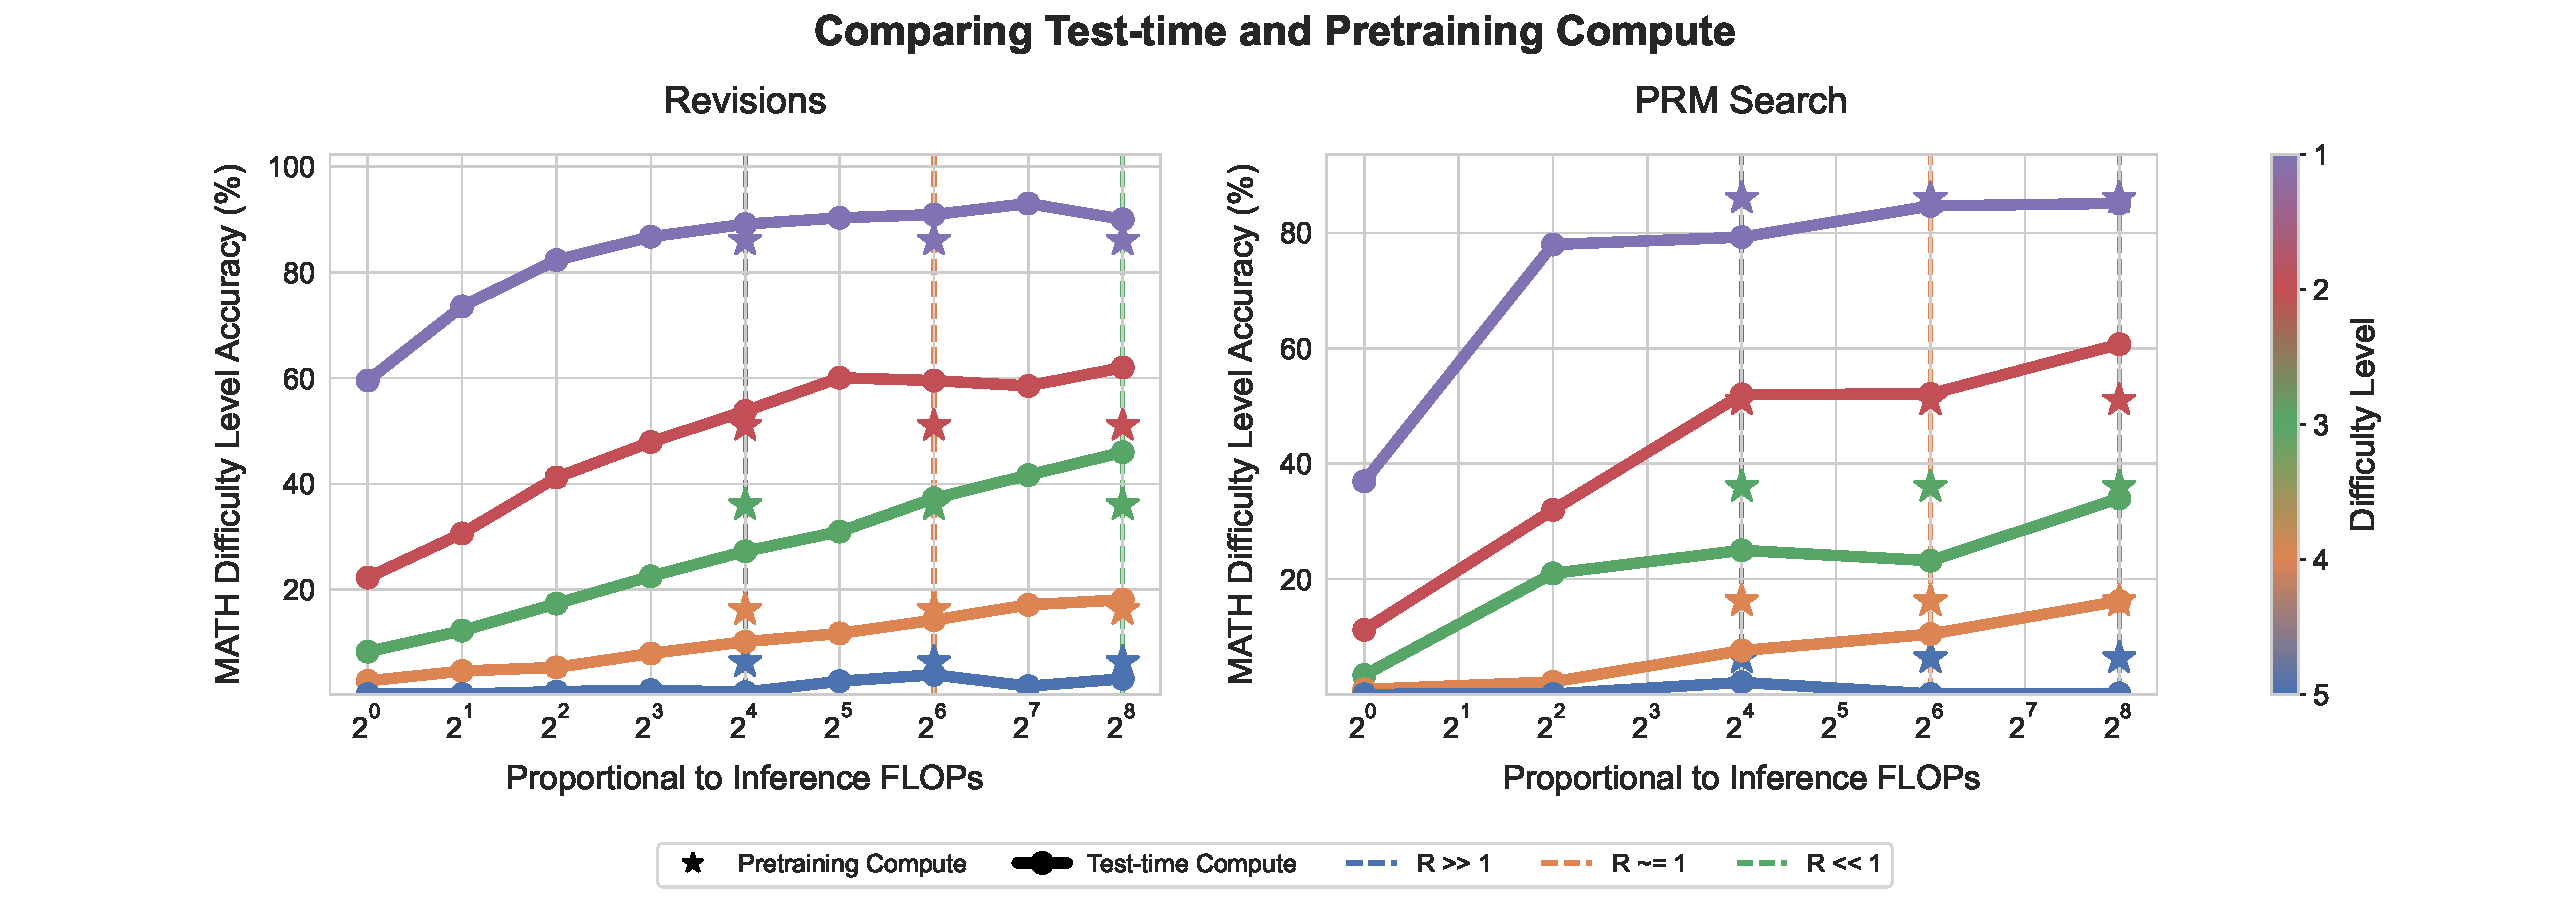
\includegraphics[trim=2.5cm 0cm 2.5cm 0cm,clip,width=.99\linewidth]{../papers/translations/testcompute/figures/comparing_test_pretrain_v8.pdf}
\caption{原图 9: FLOPs 匹配评估中, 预训练与推理时计算的权衡. 每条线表示在一个预言机难度分箱内, 用计算最优策略扩大推理时计算的表现; 左为修订, 右为搜索. 星号表示参数约大 $14$ 倍的预训练基础模型的贪心 pass@1. 横轴为推理时计算预算, 星号位于三个不同横坐标, 分别对应三种推理计算负载（$R=D_{\text{inference}}/D_{\text{pretrain}}$）下, 扩大参数与扩大推理时计算的 FLOPs 等价比较点. 星号在线下方, 意味着推理时计算比扩大参数更有效; 在线上方, 意味着扩大参数更有效. 简单问题或较低推理负载（$R\ll1$）时, 推理时计算通常能超过扩大参数; 困难问题或较高推理负载（$R\gg1$）时, 预训练是更有效的表现改进方式. }
\label{testcompute-fig:pretrain_exchange}
\end{figure}

要使用较小模型的推理时计算匹配扩大模型参数的 FLOPs, 可将小模型的推理计算乘以
\[
M+3\left(\frac{D_{\text{pretrain}}}{D_{\text{inference}}}\right)(M-1).
\]
值得注意的是, 为匹配较大模型 FLOPs 而能使用的推理计算量, 取决于比值 $D_{\text{pretrain}}/D_{\text{inference}}$. 我们将其倒数记为 $R$, 即 $D_{\text{inference}}/D_{\text{pretrain}}$. 不同生产设置或用例应有很不同的 $R$. 尤其是, 许多大规模生产设置下, 推理 token 可能显著多于预训练 token, 因此 $R\gg1$. 另一方面, 许多使用推理时计算改进模型的当代自我改进设置, 很可能生成远少于预训练数量的推理 token, 即 $R\ll1$. 因此, 可应用的推理时计算规模取决于这一比值, 我们预期不同设置得出的结论会不同. 

图\ref{testcompute-fig:pretrain_exchange}采用这种交换方式, 将计算最优扩展与参数扩大约 $14$ 倍比较. 比较三种 $R$: $0.16$（$R\ll1$）、$0.79$（$R\sim1$）、$22$（$R\gg1$）, 各对应一个推理预算. 若预期只有很困难的问题（如难度分箱 4/5）, 或有较大的 $D_{\text{inference}}$（较大的 $R$）, 往往将预算用于预训练更有效（星号位于线上方）. 若主要是简单或中等难度问题（分箱 1/2/3, 有时包括 4）, 或推理需求较低（如自我改进流水线）, 则使用推理时计算更好. 

\begin{remark}[交换预训练与推理时计算的要点]
推理时计算与预训练计算并非一比一“可互换”. 对于模型能力以内的简单、中等问题, 或推理需求较小的设置, 推理时计算很容易弥补额外预训练的作用. 但对超出基础模型能力的挑战性问题, 或推理需求较高的设置, 预训练可能更有效地改善表现. 
\end{remark}

\originalsection{8 讨论与未来工作}
\paperlabel{8}{testcompute-sec:discussion}
本工作详尽分析了改进依据验证器的搜索、或完善 LLM 提议分布的不同技术, 在数学推理中扩展推理时计算的有效性. 总体上, 从基础 LLM 能力的角度衡量的问题难度, 与某方法的有效性高度相关. 这促使我们引入推理时计算的“计算最优”扩展概念: 针对给定推理时计算预算, 规定一种依赖提示、自适应的表现改进策略. 我们发现, 这种策略能将推理时计算扩展效率提高 $2$--$4$ 倍. 在 FLOPs 匹配设置下, 将额外推理时计算的收益与额外预训练计算的收益比较, 我们首次表明: 看似简单的方法（修订、搜索）已经能在某些类型的提示上良好扩展, 收益超过将同等 FLOPs 用于预训练. 不过, 本研究也存在未来工作可处理的限制. 

\textbf{进一步改进推理时计算扩展. }本工作集中改善两个主要机制: 验证器, 以及提议分布（通过修订）. 虽然第\ref{testcompute-sec:revisions}节将验证器与修订结合, 却没有实验将 PRM 树搜索与修订结合, 也没有研究批评后修订等其他技术\cite{testcompute-madaan2023selfrefine}. 未来应研究结合多种方法, 进一步改进扩展. 此外, 我们发现, 这些方案整体上在困难问题上的收益很小; 未来应开发新的推理时计算用法, 突破这一限制. 

\textbf{快速评估问题难度. }我们将一种问题难度作为简单充分统计量, 近似计算最优推理时扩展策略. 虽然有效, 这种难度估计本身也需要相当数量的推理时计算. 未来应考虑更高效的替代难度估计方法（如预训练或微调模型, 直接预测题目难度）, 或在评估难度与尝试解题之间动态切换. 

\textbf{交错使用推理时与训练时计算. }本工作仅聚焦推理时计算的扩展, 以及它能在多大程度上与额外预训练互换. 但我们设想, 未来额外推理时计算产生的输出可以蒸馏回基础 LLM, 形成能处理开放式自然语言的迭代自我改进循环. 因此, 未来应扩展本研究, 考察如何用推理时计算的输出改进基础 LLM 本身. 

\subsection*{致谢}
\label{testcompute-acknowledgements}
感谢 Yi Su、Rishabh Agarwal、Yinlam Chow、Aleksandra Faust、Vincent Zhuang、George Tucker、Hao Liu、Jiayi Pan、Ethan Dyer、Behnam Neyshabur、Xavier Garcia、Yamini Bansal、Lampros Lamprou、Yuxiao Qu、Amrith Setlur 对早期稿件的反馈与讨论. 我们将有关想法与讨论, 以及具体展示成对样本生成有望训练修订模型的实验、文献\cite{testcompute-anonymousrevisions}中基于编辑距离采样的实验, 归功并致谢于 Rishabh Agarwal、Vincent Zhuang、Yi Su、Avi Singh. 感谢 Slav Petrov 的领导支持. 

% 参考文献完整保留原作者、原题、出版信息及链接. 
\begin{thebibliography}{51}
\label{testcompute-references}
\providecommand{\natexlab}[1]{#1}
\providecommand{\url}[1]{\texttt{#1}}
\expandafter\ifx\csname urlstyle\endcsname\relax
  \providecommand{\doi}[1]{doi: #1}\else
  \providecommand{\doi}{doi: \begingroup \urlstyle{rm}\Url}\fi

\bibitem{testcompute-anonymousrevisions}
Training revision models with synthetic data.
\newblock Coming soon, 2024.

\bibitem{testcompute-andrieu2003introduction}
C.~Andrieu, N.~De~Freitas, A.~Doucet, and M.~I. Jordan.
\newblock An introduction to mcmc for machine learning.
\newblock 2003.

\bibitem{testcompute-anil2023palm}
R.~Anil, A.~M. Dai, O.~Firat, M.~Johnson, D.~Lepikhin, A.~Passos, S.~Shakeri, E.~Taropa, P.~Bailey, Z.~Chen, E.~Chu, J.~H. Clark, L.~E. Shafey, Y.~Huang, K.~Meier-Hellstern, G.~Mishra, E.~Moreira, M.~Omernick, K.~Robinson, S.~Ruder, Y.~Tay, K.~Xiao, Y.~Xu, Y.~Zhang, G.~H. Abrego, J.~Ahn, J.~Austin, P.~Barham, J.~Botha, J.~Bradbury, S.~Brahma, K.~Brooks, M.~Catasta, Y.~Cheng, C.~Cherry, C.~A. Choquette-Choo, A.~Chowdhery, C.~Crepy, S.~Dave, M.~Dehghani, S.~Dev, J.~Devlin, M.~Díaz, N.~Du, E.~Dyer, V.~Feinberg, F.~Feng, V.~Fienber, M.~Freitag, X.~Garcia, S.~Gehrmann, L.~Gonzalez, G.~Gur-Ari, S.~Hand, H.~Hashemi, L.~Hou, J.~Howland, A.~Hu, J.~Hui, J.~Hurwitz, M.~Isard, A.~Ittycheriah, M.~Jagielski, W.~Jia, K.~Kenealy, M.~Krikun, S.~Kudugunta, C.~Lan, K.~Lee, B.~Lee, E.~Li, M.~Li, W.~Li, Y.~Li, J.~Li, H.~Lim, H.~Lin, Z.~Liu, F.~Liu, M.~Maggioni, A.~Mahendru, J.~Maynez, V.~Misra, M.~Moussalem, Z.~Nado, J.~Nham, E.~Ni, A.~Nystrom, A.~Parrish, M.~Pellat, M.~Polacek, A.~Polozov, R.~Pope, S.~Qiao, E.~Reif, B.~Richter,
  P.~Riley, A.~C. Ros, A.~Roy, B.~Saeta, R.~Samuel, R.~Shelby, A.~Slone, D.~Smilkov, D.~R. So, D.~Sohn, S.~Tokumine, D.~Valter, V.~Vasudevan, K.~Vodrahalli, X.~Wang, P.~Wang, Z.~Wang, T.~Wang, J.~Wieting, Y.~Wu, K.~Xu, Y.~Xu, L.~Xue, P.~Yin, J.~Yu, Q.~Zhang, S.~Zheng, C.~Zheng, W.~Zhou, D.~Zhou, S.~Petrov, and Y.~Wu.
\newblock Palm 2 technical report, 2023.

\bibitem{testcompute-bai2022constitutional}
Y.~Bai, S.~Kadavath, S.~Kundu, A.~Askell, J.~Kernion, A.~Jones, A.~Chen, A.~Goldie, A.~Mirhoseini, C.~McKinnon, C.~Chen, C.~Olsson, C.~Olah, D.~Hernandez, D.~Drain, D.~Ganguli, D.~Li, E.~Tran-Johnson, E.~Perez, J.~Kerr, J.~Mueller, J.~Ladish, J.~Landau, K.~Ndousse, K.~Lukosuite, L.~Lovitt, M.~Sellitto, N.~Elhage, N.~Schiefer, N.~Mercado, N.~DasSarma, R.~Lasenby, R.~Larson, S.~Ringer, S.~Johnston, S.~Kravec, S.~E. Showk, S.~Fort, T.~Lanham, T.~Telleen-Lawton, T.~Conerly, T.~Henighan, T.~Hume, S.~R. Bowman, Z.~Hatfield-Dodds, B.~Mann, D.~Amodei, N.~Joseph, S.~McCandlish, T.~Brown, and J.~Kaplan.
\newblock Constitutional ai: Harmlessness from ai feedback, 2022.

\bibitem{testcompute-blakeney2024doesdatasparkjoy}
C.~Blakeney, M.~Paul, B.~W. Larsen, S.~Owen, and J.~Frankle.
\newblock Does your data spark joy? performance gains from domain upsampling at the end of training, 2024.
\newblock URL \url{https://arxiv.org/abs/2406.03476}.

\bibitem{testcompute-chen2024alphamath}
G.~Chen, M.~Liao, C.~Li, and K.~Fan.
\newblock Alphamath almost zero: process supervision without process, 2024.

\bibitem{testcompute-cobbe2021training}
K.~Cobbe, V.~Kosaraju, M.~Bavarian, M.~Chen, H.~Jun, L.~Kaiser, M.~Plappert, J.~Tworek, J.~Hilton, R.~Nakano, C.~Hesse, and J.~Schulman.
\newblock Training verifiers to solve math word problems, 2021.

\bibitem{testcompute-du2023improving}
Y.~Du, S.~Li, A.~Torralba, J.~B. Tenenbaum, and I.~Mordatch.
\newblock Improving factuality and reasoning in language models through multiagent debate, 2023.

\bibitem{testcompute-evans1984heuristic}
J.~S. B.~T. Evans.
\newblock Heuristic and analytic processes in reasoning.
\newblock \emph{British Journal of Psychology}, 75(4):\penalty0 451--468, 1984.

\bibitem{testcompute-feng2024alphazerolike}
X.~Feng, Z.~Wan, M.~Wen, S.~M. McAleer, Y.~Wen, W.~Zhang, and J.~Wang.
\newblock Alphazero-like tree-search can guide large language model decoding and training, 2024.

\bibitem{testcompute-gao2023palprogramaidedlanguagemodels}
L.~Gao, A.~Madaan, S.~Zhou, U.~Alon, P.~Liu, Y.~Yang, J.~Callan, and G.~Neubig.
\newblock Pal: Program-aided language models, 2023.
\newblock URL \url{https://arxiv.org/abs/2211.10435}.

\bibitem{testcompute-goyal2024thinkspeaktraininglanguage}
S.~Goyal, Z.~Ji, A.~S. Rawat, A.~K. Menon, S.~Kumar, and V.~Nagarajan.
\newblock Think before you speak: Training language models with pause tokens, 2024.
\newblock URL \url{https://arxiv.org/abs/2310.02226}.

\bibitem{testcompute-hendrycks2021measuring}
D.~Hendrycks, C.~Burns, S.~Kadavath, A.~Arora, S.~Basart, E.~Tang, D.~Song, and J.~Steinhardt.
\newblock Measuring mathematical problem solving with the math dataset, 2021.

\bibitem{testcompute-hoffmann2022training}
J.~Hoffmann, S.~Borgeaud, A.~Mensch, E.~Buchatskaya, T.~Cai, E.~Rutherford, D.~de~Las~Casas, L.~A. Hendricks, J.~Welbl, A.~Clark, T.~Hennigan, E.~Noland, K.~Millican, G.~van~den Driessche, B.~Damoc, A.~Guy, S.~Osindero, K.~Simonyan, E.~Elsen, J.~W. Rae, O.~Vinyals, and L.~Sifre.
\newblock Training compute-optimal large language models, 2022.

\bibitem{testcompute-huang2023large}
J.~Huang, X.~Chen, S.~Mishra, H.~S. Zheng, A.~W. Yu, X.~Song, and D.~Zhou.
\newblock Large language models cannot self-correct reasoning yet, 2023.

\bibitem{testcompute-jones2021scalingscalinglawsboard}
A.~L. Jones.
\newblock Scaling scaling laws with board games, 2021.
\newblock URL \url{https://arxiv.org/abs/2104.03113}.

\bibitem{testcompute-kahneman2003maps}
D.~Kahneman.
\newblock Maps of bounded rationality: Psychology for behavioral economics.
\newblock \emph{The American Economic Review}, 93(5):\penalty0 1449--1475, 2003.

\bibitem{testcompute-kahneman2013thinking}
D.~Kahneman.
\newblock \emph{Thinking, fast and slow}.
\newblock Farrar, Straus and Giroux, New York, first paperback edition edition, 2013.

\bibitem{testcompute-kocsis2006bandit}
L.~Kocsis and C.~Szepesv{'a}ri.
\newblock Bandit based monte-carlo planning.
\newblock In \emph{European conference on machine learning}, pages 282--293. Springer, 2006.

\bibitem{testcompute-lewkowycz2022solving}
A.~Lewkowycz, A.~Andreassen, D.~Dohan, E.~Dyer, H.~Michalewski, V.~Ramasesh, A.~Slone, C.~Anil, I.~Schlag, T.~Gutman-Solo, Y.~Wu, B.~Neyshabur, G.~Gur-Ari, and V.~Misra.
\newblock Solving quantitative reasoning problems with language models, 2022.

\bibitem{testcompute-li2023making}
Y.~Li, Z.~Lin, S.~Zhang, Q.~Fu, B.~Chen, J.-G. Lou, and W.~Chen.
\newblock Making large language models better reasoners with step-aware verifier, 2023.

\bibitem{testcompute-lightman2023lets}
H.~Lightman, V.~Kosaraju, Y.~Burda, H.~Edwards, B.~Baker, T.~Lee, J.~Leike, J.~Schulman, I.~Sutskever, and K.~Cobbe.
\newblock Let's verify step by step, 2023.

\bibitem{testcompute-madaan2023selfrefine}
A.~Madaan, N.~Tandon, P.~Gupta, S.~Hallinan, L.~Gao, S.~Wiegreffe, U.~Alon, N.~Dziri, S.~Prabhumoye, Y.~Yang, S.~Gupta, B.~P. Majumder, K.~Hermann, S.~Welleck, A.~Yazdanbakhsh, and P.~Clark.
\newblock Self-refine: Iterative refinement with self-feedback, 2023.

\bibitem{testcompute-llmcriticscatchbugs}
N.~McAleese, R.~Pokorny, J.~F. Cerón~Uribe, E.~Nitishinskaya, M.~Trębacz, and J.~Leike.
\newblock Llm critics help catch llm bugs.
\newblock \emph{OpenAI}, 2024.

\bibitem{testcompute-openai2024gpt4}
OpenAI.
\newblock Gpt-4 technical report, 2024.

\bibitem{testcompute-qin2023toolllmfacilitatinglargelanguage}
Y.~Qin, S.~Liang, Y.~Ye, K.~Zhu, L.~Yan, Y.~Lu, Y.~Lin, X.~Cong, X.~Tang, B.~Qian, S.~Zhao, L.~Hong, R.~Tian, R.~Xie, J.~Zhou, M.~Gerstein, D.~Li, Z.~Liu, and M.~Sun.
\newblock Toolllm: Facilitating large language models to master 16000+ real-world apis, 2023.
\newblock URL \url{https://arxiv.org/abs/2307.16789}.

\bibitem{testcompute-qu2024toollearninglargelanguage}
C.~Qu, S.~Dai, X.~Wei, H.~Cai, S.~Wang, D.~Yin, J.~Xu, and J.-R. Wen.
\newblock Tool learning with large language models: A survey, 2024{\natexlab{a}}.
\newblock URL \url{https://arxiv.org/abs/2405.17935}.

\bibitem{testcompute-qu2024recursive}
Y.~Qu, T.~Zhang, N.~Garg, and A.~Kumar.
\newblock Recursive introspection: Teaching foundation models how to self-improve.
\newblock 2024{\natexlab{b}}.

\bibitem{testcompute-sardana2023chinchillaoptimal}
N.~Sardana and J.~Frankle.
\newblock Beyond chinchilla-optimal: Accounting for inference in language model scaling laws, 2023.

\bibitem{testcompute-saunders2022selfcritiquing}
W.~Saunders, C.~Yeh, J.~Wu, S.~Bills, L.~Ouyang, J.~Ward, and J.~Leike.
\newblock Self-critiquing models for assisting human evaluators, 2022.

\bibitem{testcompute-setlur2024rl}
A.~Setlur, S.~Garg, X.~Geng, N.~Garg, V.~Smith, and A.~Kumar.
\newblock Rl on incorrect synthetic data scales the efficiency of llm math reasoning by eight-fold.
\newblock \emph{arXiv preprint arXiv:2406.14532}, 2024.

\bibitem{testcompute-shao2024deepseekmath}
Z.~Shao, P.~Wang, Q.~Zhu, R.~Xu, J.~Song, X.~Bi, H.~Zhang, M.~Zhang, Y.~K. Li, Y.~Wu, and D.~Guo.
\newblock Deepseekmath: Pushing the limits of mathematical reasoning in open language models, 2024.

\bibitem{testcompute-sharma2024criticalevaluationaifeedback}
A.~Sharma, S.~Keh, E.~Mitchell, C.~Finn, K.~Arora, and T.~Kollar.
\newblock A critical evaluation of ai feedback for aligning large language models, 2024.
\newblock URL \url{https://arxiv.org/abs/2402.12366}.

\bibitem{testcompute-shinn2023reflexion}
N.~Shinn, F.~Cassano, E.~Berman, A.~Gopinath, K.~Narasimhan, and S.~Yao.
\newblock Reflexion: Language agents with verbal reinforcement learning, 2023.

\bibitem{testcompute-singh2024human}
A.~Singh, J.~D. Co-Reyes, R.~Agarwal, A.~Anand, P.~Patil, X.~Garcia, P.~J. Liu, J.~Harrison, J.~Lee, K.~Xu, A.~Parisi, A.~Kumar, A.~Alemi, A.~Rizkowsky, A.~Nova, B.~Adlam, B.~Bohnet, G.~Elsayed, H.~Sedghi, I.~Mordatch, I.~Simpson, I.~Gur, J.~Snoek, J.~Pennington, J.~Hron, K.~Kenealy, K.~Swersky, K.~Mahajan, L.~Culp, L.~Xiao, M.~L. Bileschi, N.~Constant, R.~Novak, R.~Liu, T.~Warkentin, Y.~Qian, Y.~Bansal, E.~Dyer, B.~Neyshabur, J.~Sohl-Dickstein, and N.~Fiedel.
\newblock Beyond human data: Scaling self-training for problem-solving with language models, 2024.

\bibitem{testcompute-predictemergence}
C.~Snell, E.~Wallace, D.~Klein, and S.~Levine.
\newblock Predicting emergent capabilities by finetuning.
\newblock \emph{Conference on Language Modeling 2024}, 2024.

\bibitem{testcompute-stechly2023gpt4}
K.~Stechly, M.~Marquez, and S.~Kambhampati.
\newblock Gpt-4 doesn't know it's wrong: An analysis of iterative prompting for reasoning problems, 2023.

\bibitem{testcompute-suttonrlbook}
R.~S. Sutton and A.~G. Barto.
\newblock \emph{Reinforcement learning: An introduction}.
\newblock Second edition, 2018.

\bibitem{testcompute-geminiteam2024gemini}
G.~Team.
\newblock Gemini 1.5: Unlocking multimodal understanding across millions of tokens of context, 2024.

\bibitem{testcompute-tian2024selfimprovement}
Y.~Tian, B.~Peng, L.~Song, L.~Jin, D.~Yu, H.~Mi, and D.~Yu.
\newblock Toward self-improvement of llms via imagination, searching, and criticizing, 2024.

\bibitem{testcompute-touvron2023llama2openfoundation}
H.~Touvron, L.~Martin, K.~Stone, P.~Albert, A.~Almahairi, Y.~Babaei, N.~Bashlykov, S.~Batra, P.~Bhargava, S.~Bhosale, D.~Bikel, L.~Blecher, C.~C. Ferrer, M.~Chen, G.~Cucurull, D.~Esiobu, J.~Fernandes, J.~Fu, W.~Fu, B.~Fuller, C.~Gao, V.~Goswami, N.~Goyal, A.~Hartshorn, S.~Hosseini, R.~Hou, H.~Inan, M.~Kardas, V.~Kerkez, M.~Khabsa, I.~Kloumann, A.~Korenev, P.~S. Koura, M.-A. Lachaux, T.~Lavril, J.~Lee, D.~Liskovich, Y.~Lu, Y.~Mao, X.~Martinet, T.~Mihaylov, P.~Mishra, I.~Molybog, Y.~Nie, A.~Poulton, J.~Reizenstein, R.~Rungta, K.~Saladi, A.~Schelten, R.~Silva, E.~M. Smith, R.~Subramanian, X.~E. Tan, B.~Tang, R.~Taylor, A.~Williams, J.~X. Kuan, P.~Xu, Z.~Yan, I.~Zarov, Y.~Zhang, A.~Fan, M.~Kambadur, S.~Narang, A.~Rodriguez, R.~Stojnic, S.~Edunov, and T.~Scialom.
\newblock Llama 2: Open foundation and fine-tuned chat models, 2023.
\newblock URL \url{https://arxiv.org/abs/2307.09288}.

\bibitem{testcompute-uesato2022solving}
J.~Uesato, N.~Kushman, R.~Kumar, F.~Song, N.~Siegel, L.~Wang, A.~Creswell, G.~Irving, and I.~Higgins.
\newblock Solving math word problems with process- and outcome-based feedback, 2022.

\bibitem{testcompute-valmeekam2023large}
K.~Valmeekam, M.~Marquez, and S.~Kambhampati.
\newblock Can large language models really improve by self-critiquing their own plans?, 2023.

\bibitem{testcompute-epoch2023tradingoffcomputeintrainingandinference}
P.~Villalobos and D.~Atkinson.
\newblock Trading off compute in training and inference, 2023.
\newblock URL \url{https://epochai.org/blog/trading-off-compute-in-training-and-inference}.
\newblock Accessed: 2024-07-03.

\bibitem{testcompute-wang2023mathshepherd}
P.~Wang, L.~Li, Z.~Shao, R.~X. Xu, D.~Dai, Y.~Li, D.~Chen, Y.~Wu, and Z.~Sui.
\newblock Math-shepherd: Verify and reinforce llms step-by-step without human annotations, 2023.

\bibitem{testcompute-wang2024hypothesissearchinductivereasoning}
R.~Wang, E.~Zelikman, G.~Poesia, Y.~Pu, N.~Haber, and N.~D. Goodman.
\newblock Hypothesis search: Inductive reasoning with language models, 2024.
\newblock URL \url{https://arxiv.org/abs/2309.05660}.

\bibitem{testcompute-wei2023chainofthought}
J.~Wei, X.~Wang, D.~Schuurmans, M.~Bosma, B.~Ichter, F.~Xia, E.~Chi, Q.~Le, and D.~Zhou.
\newblock Chain-of-thought prompting elicits reasoning in large language models, 2023.

\bibitem{testcompute-yao2023tree}
S.~Yao, D.~Yu, J.~Zhao, I.~Shafran, T.~L. Griffiths, Y.~Cao, and K.~Narasimhan.
\newblock Tree of thoughts: Deliberate problem solving with large language models, 2023.

\bibitem{testcompute-yuan2023scaling}
Z.~Yuan, H.~Yuan, C.~Li, G.~Dong, K.~Lu, C.~Tan, C.~Zhou, and J.~Zhou.
\newblock Scaling relationship on learning mathematical reasoning with large language models, 2023.

\bibitem{testcompute-zelikman2022star}
E.~Zelikman, Y.~Wu, J.~Mu, and N.~D. Goodman.
\newblock Star: Bootstrapping reasoning with reasoning, 2022.

\bibitem{testcompute-zelikman2024quietstarlanguagemodelsteach}
E.~Zelikman, G.~Harik, Y.~Shao, V.~Jayasiri, N.~Haber, and N.~D. Goodman.
\newblock Quiet-star: Language models can teach themselves to think before speaking, 2024.
\newblock URL \url{https://arxiv.org/abs/2403.09629}.

\end{thebibliography}

\markboth{\thechapter\quad 推理时计算的最优扩展}{}

\originalsection{附录 A 相关工作}
\paperlabel{A}{testcompute-app:related_work}
\textbf{语言模型推理. }近年来, 语言模型在具有挑战性的数学推理任务上的表现迅速提高\cite{testcompute-lewkowycz2022solving,testcompute-geminiteam2024gemini,testcompute-openai2024gpt4,testcompute-shao2024deepseekmath,testcompute-lightman2023lets}. 这些改进可归因于四个主要因素: \textbf{1）}在大规模数学数据语料上继续预训练\cite{testcompute-lewkowycz2022solving,testcompute-geminiteam2024gemini,testcompute-shao2024deepseekmath,testcompute-lightman2023lets}; \textbf{2）}通过在特定推理任务上用强化学习微调进行有针对性的优化\cite{testcompute-singh2024human,testcompute-zelikman2022star,testcompute-shao2024deepseekmath,testcompute-yuan2023scaling}, 或让模型迭代批评、修订答案\cite{testcompute-bai2022constitutional,testcompute-madaan2023selfrefine,testcompute-du2023improving,testcompute-saunders2022selfcritiquing}, 改进 LLM 的提议分布; \textbf{3）}通过微调验证器, 让 LLM 受益于额外推理时计算\cite{testcompute-lightman2023lets,testcompute-cobbe2021training,testcompute-uesato2022solving,testcompute-wang2023mathshepherd,testcompute-yao2023tree,testcompute-feng2024alphazerolike,testcompute-chen2024alphamath,testcompute-tian2024selfimprovement}. 本工作以第二、第三条研究路线为基础, 分析可以在多大程度上通过 1）完善 LLM 提议分布, 2）依据验证器搜索, 来改善推理时计算扩展. 
\begin{remark}
译者注: 原文称“四个主要因素”, 实际列出三个编号项; 这里保留原文, 不补造第四项. 
\end{remark}

\textbf{分析推理时计算扩展. }Jones\cite{testcompute-jones2021scalingscalinglawsboard}曾研究将蒙特卡洛树搜索应用于 Hex 棋时, 训练时与测试时计算的权衡. 我们则分析完整规模的语言模型数学推理问题. Epoch 的综述\cite{testcompute-epoch2023tradingoffcomputeintrainingandinference}分析多个领域的训练与推理权衡, 但其语言模型分析多聚焦已知真实答案的推理时计算扩展设置. 我们则聚焦不知道真实答案的设置. 此外, 强化学习文献中的许多工作提出 MCTS\cite{testcompute-kocsis2006bandit}等方法, 试图在测试时与训练时计算间权衡, 实现迭代自博弈. 本研究发现可帮助开发能在开放式自然语言上运行的类似算法. 

\textbf{用推理时计算增强 LLM. }除验证器与修订外, 许多工作还提出让语言模型利用推理时计算进行推理的替代方法. 例如, Wang 等人\cite{testcompute-wang2024hypothesissearchinductivereasoning}开展层次假设搜索, 以获得归纳推理能力. 相关工作提出测试时为语言模型配备工具, 可大幅提高下游任务表现\cite{testcompute-gao2023palprogramaidedlanguagemodels,testcompute-qin2023toolllmfacilitatinglargelanguage,testcompute-qu2024toollearninglargelanguage}. 另有若干工作提出无监督学习思考 token 的方法\cite{testcompute-zelikman2024quietstarlanguagemodelsteach,testcompute-goyal2024thinkspeaktraininglanguage}, 使模型更有效地利用采样更长序列带来的额外推理时计算. 虽然本工作只分析两种主要机制（验证器与修订）, 我们的许多分析方法（如按难度计算最优扩展）原则上也可应用于其他扩展方法, 我们认为这是值得研究的未来方向. 

\originalsection{附录 B 额外修订结果}
\paperlabel{B}{testcompute-app:additional_revision}
图\ref{testcompute-fig:revision_maj_additional}给出 PaLM 2-S* 修订模型使用多数投票选择的额外结果. 其趋势基本类似图\ref{testcompute-fig:iso_revisions}中的验证器选择结果. 
\begin{figure}[htbp]
\centering
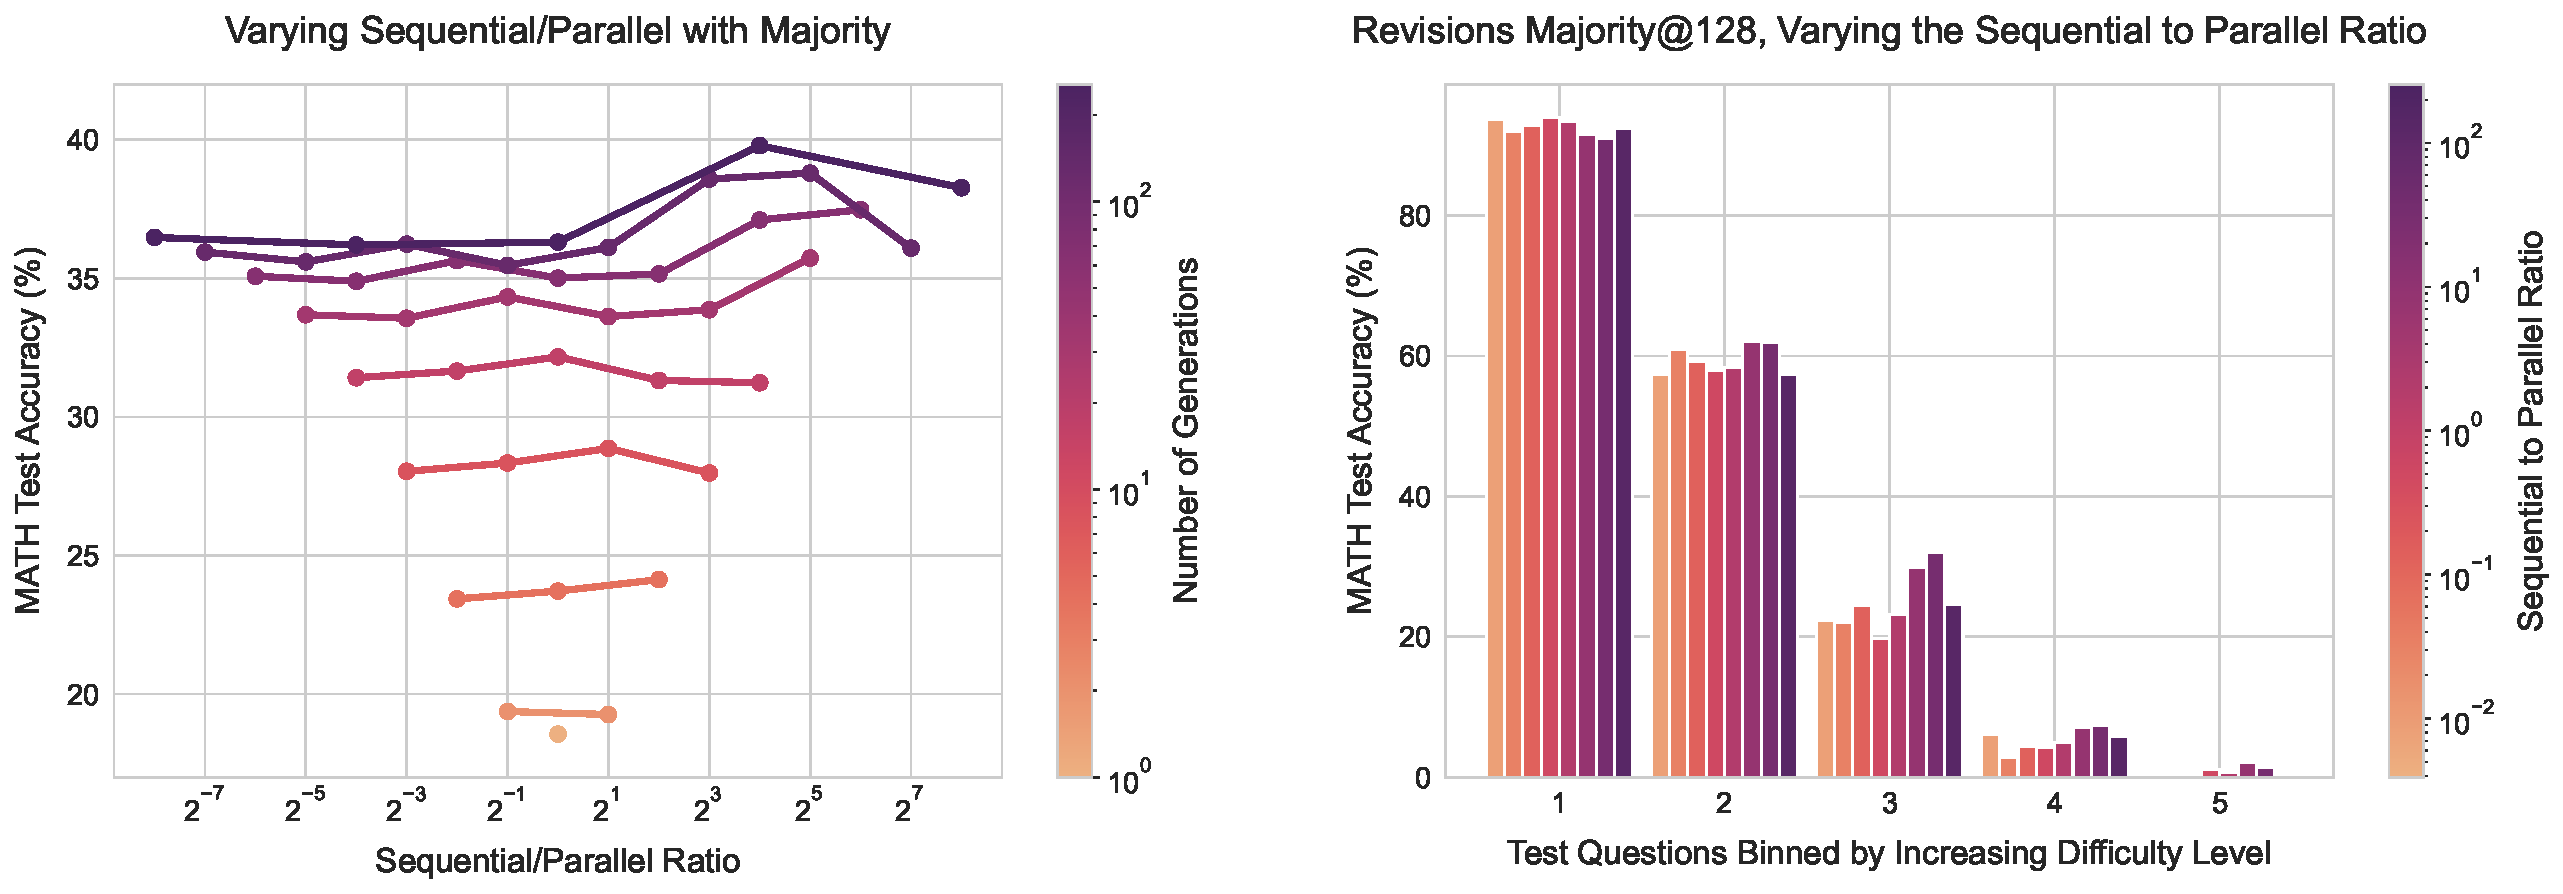
\includegraphics[width=.99\linewidth]{../papers/translations/testcompute/figures/iso_gens_majority_difficulty.pdf}
\caption{原图 10: 改变生成预算用于顺序与并行样本的比例, 用多数投票而非验证器选择答案. \textbf{左: }每条线对应固定预算; 比例变化时, 与验证器情况类似, 存在理想的顺序与并行推理时计算比例. \textbf{右: }跨难度分箱分析, 简单问题大多不随该比例变化; 困难问题则存在理想比例. }
\label{testcompute-fig:revision_maj_additional}
\end{figure}

\originalsection{附录 C 无监督难度分箱}
\paperlabel{C}{testcompute-app:unsupervised_difficulty}
无需预言机真实正确性信息, 我们将每题 $2048$ 个样本的 PRM 最终答案得分取平均, 得到对应问题的价值估计. 然后将测试集各题的价值划为五个五分位组（流程与预言机难度分箱相同）. 称之为“预测难度”, 而非“预言机难度”. 严格说, 此流程成本极高, 因为要生成大量样本. 虽然分析没有计入此成本, 在实际生产设置中, 这会造成问题. 更高效的方法是微调模型, 让其给定问题直接预测正确性. 本工作没有探索此方法, 将更便宜难度估计方法的研究留给未来. 

图\ref{testcompute-fig:search_unsupervised_difficulty}绘出这些分箱下的 PRM 搜索结果, 图\ref{testcompute-fig:revisions_unsupervised_difficulty}给出对应修订结果. 两种设置中, 预测分箱均显示出与预言机分箱类似的趋势. 
\begin{figure}[htbp]
\centering
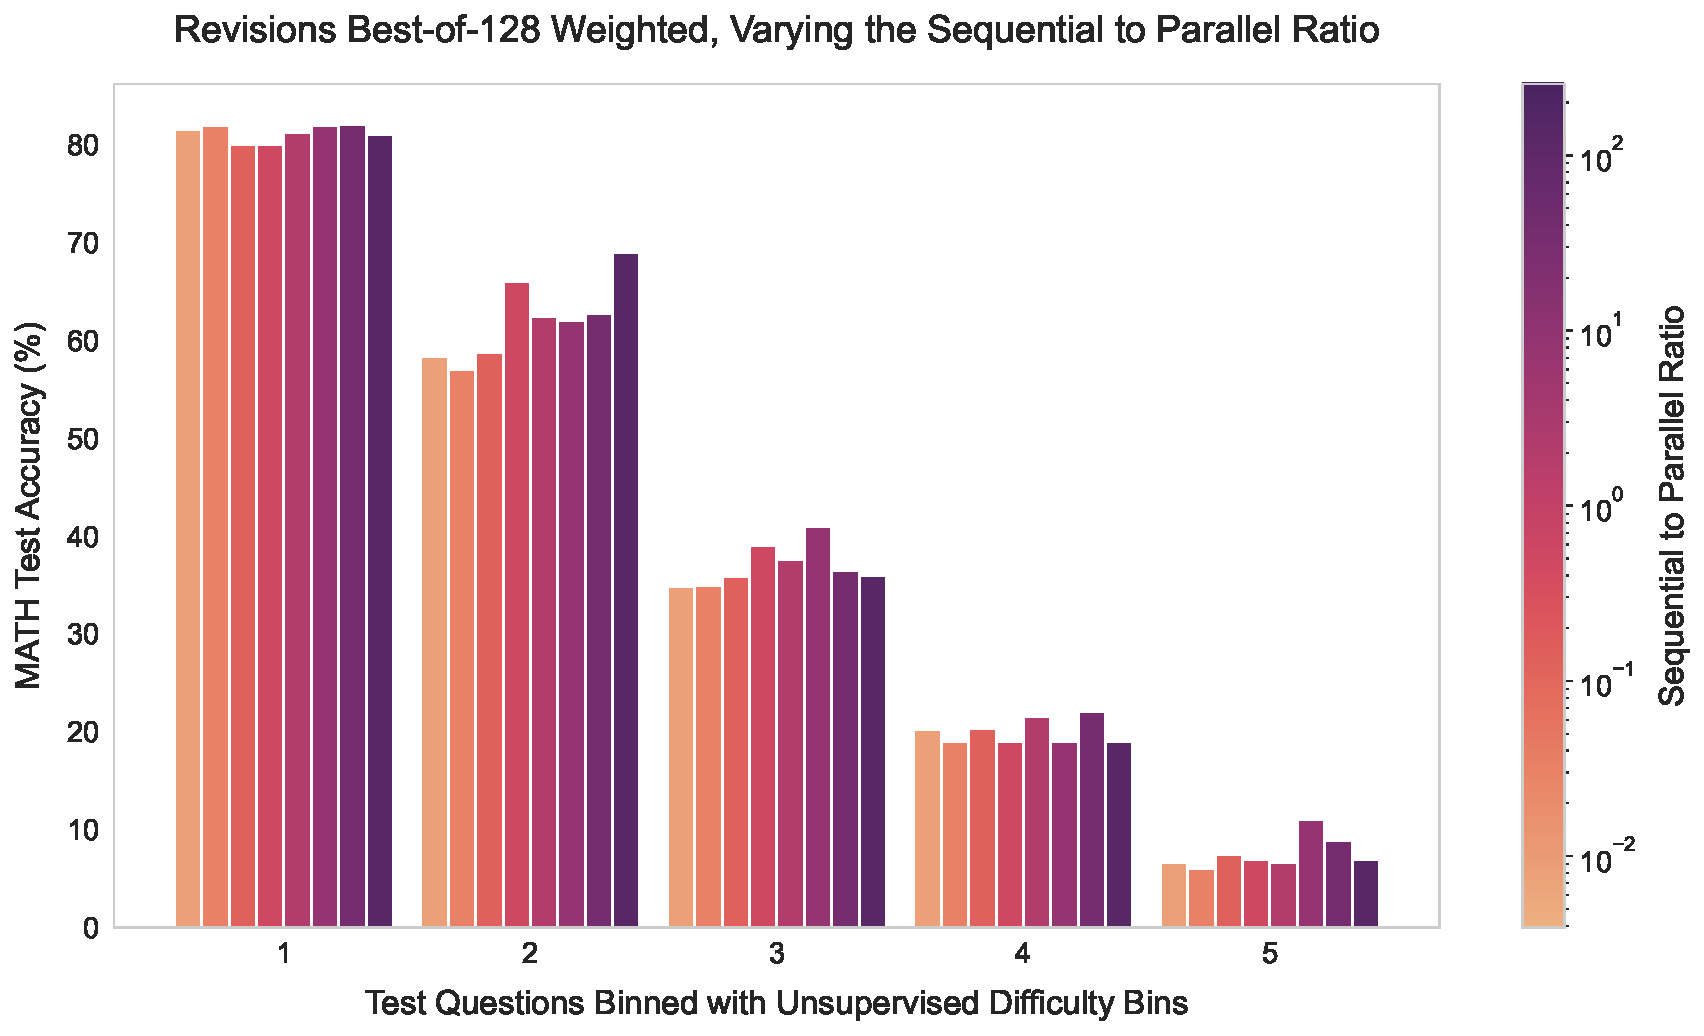
\includegraphics[width=.49\linewidth]{../papers/translations/testcompute/figures/bon_unsupervised_difficulty_output.pdf}
\label{testcompute-fig:bon_unsupervised_difficulty_output}
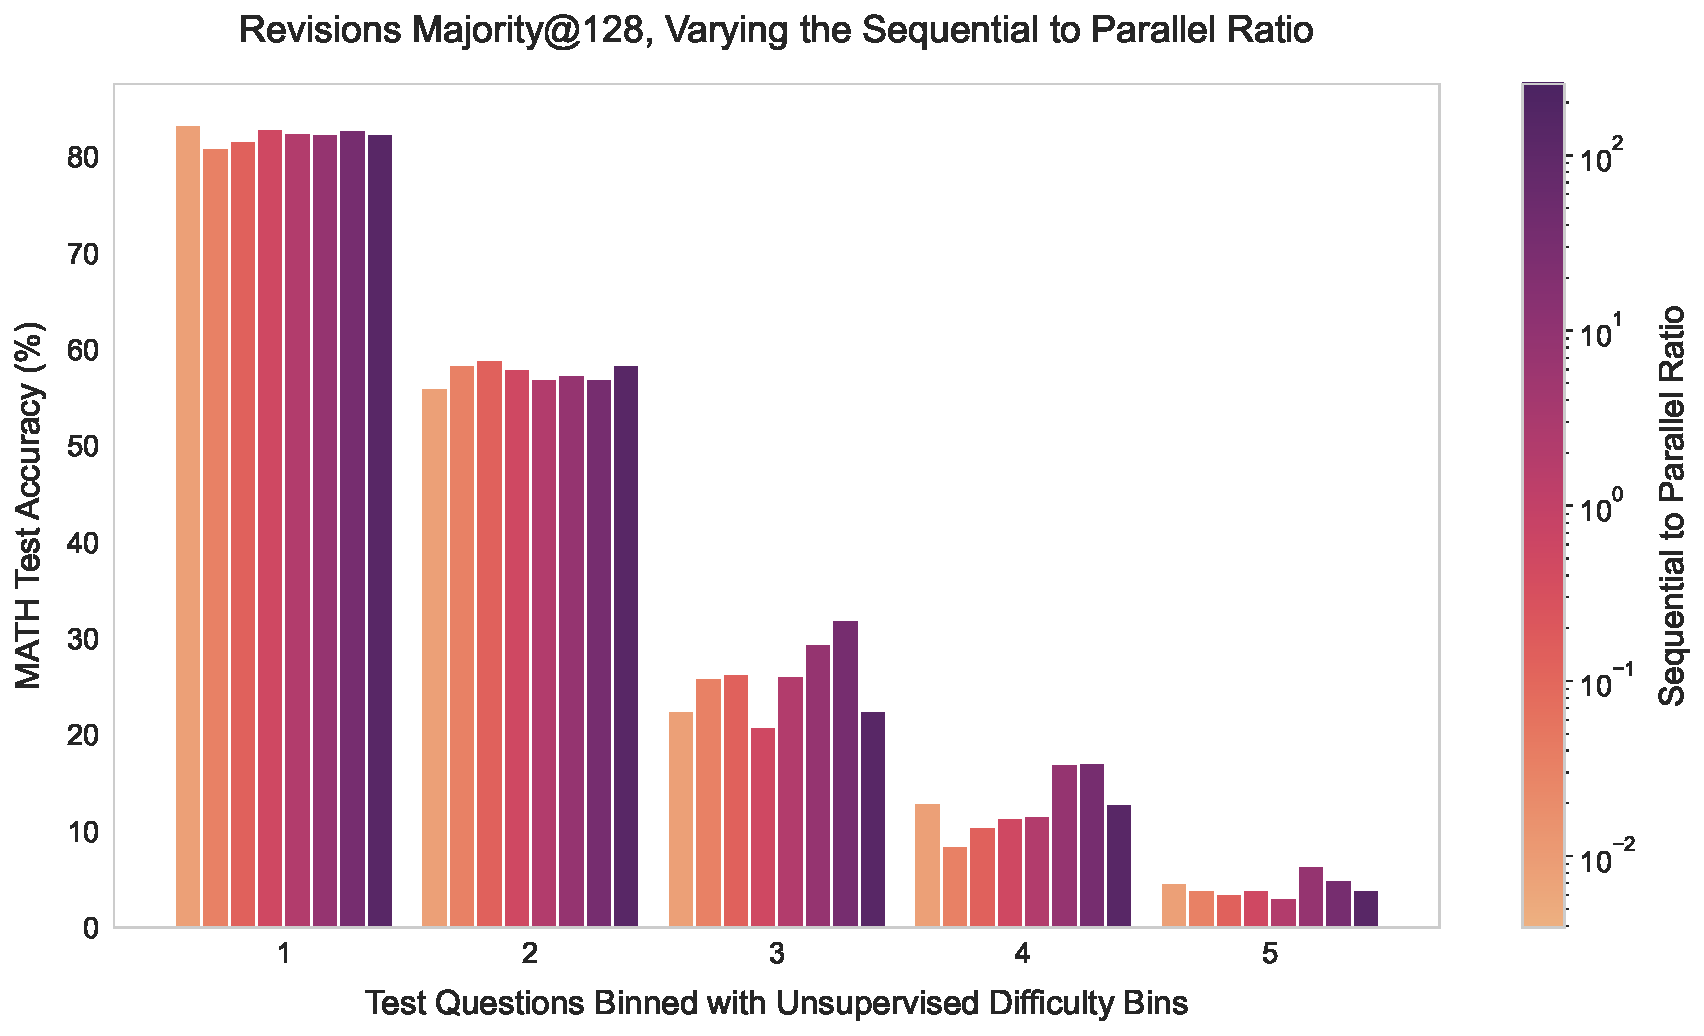
\includegraphics[width=.49\linewidth]{../papers/translations/testcompute/figures/maj_unsupervised_difficulty_output.pdf}
\label{testcompute-fig:maj_unsupervised_difficulty_output}
\caption{原图 11: 用 PaLM 2-S* PRM, 在没有真实正确性信息时, 为修订计算难度分箱. 左为验证器选择, 右为多数投票选择. 与图\ref{testcompute-fig:iso_revisions}、\ref{testcompute-fig:revision_maj_additional}的真实信息分箱基本呈现相似表现趋势. }
\label{testcompute-fig:revisions_unsupervised_difficulty}
\end{figure}
\begin{figure}[htbp]
\centering
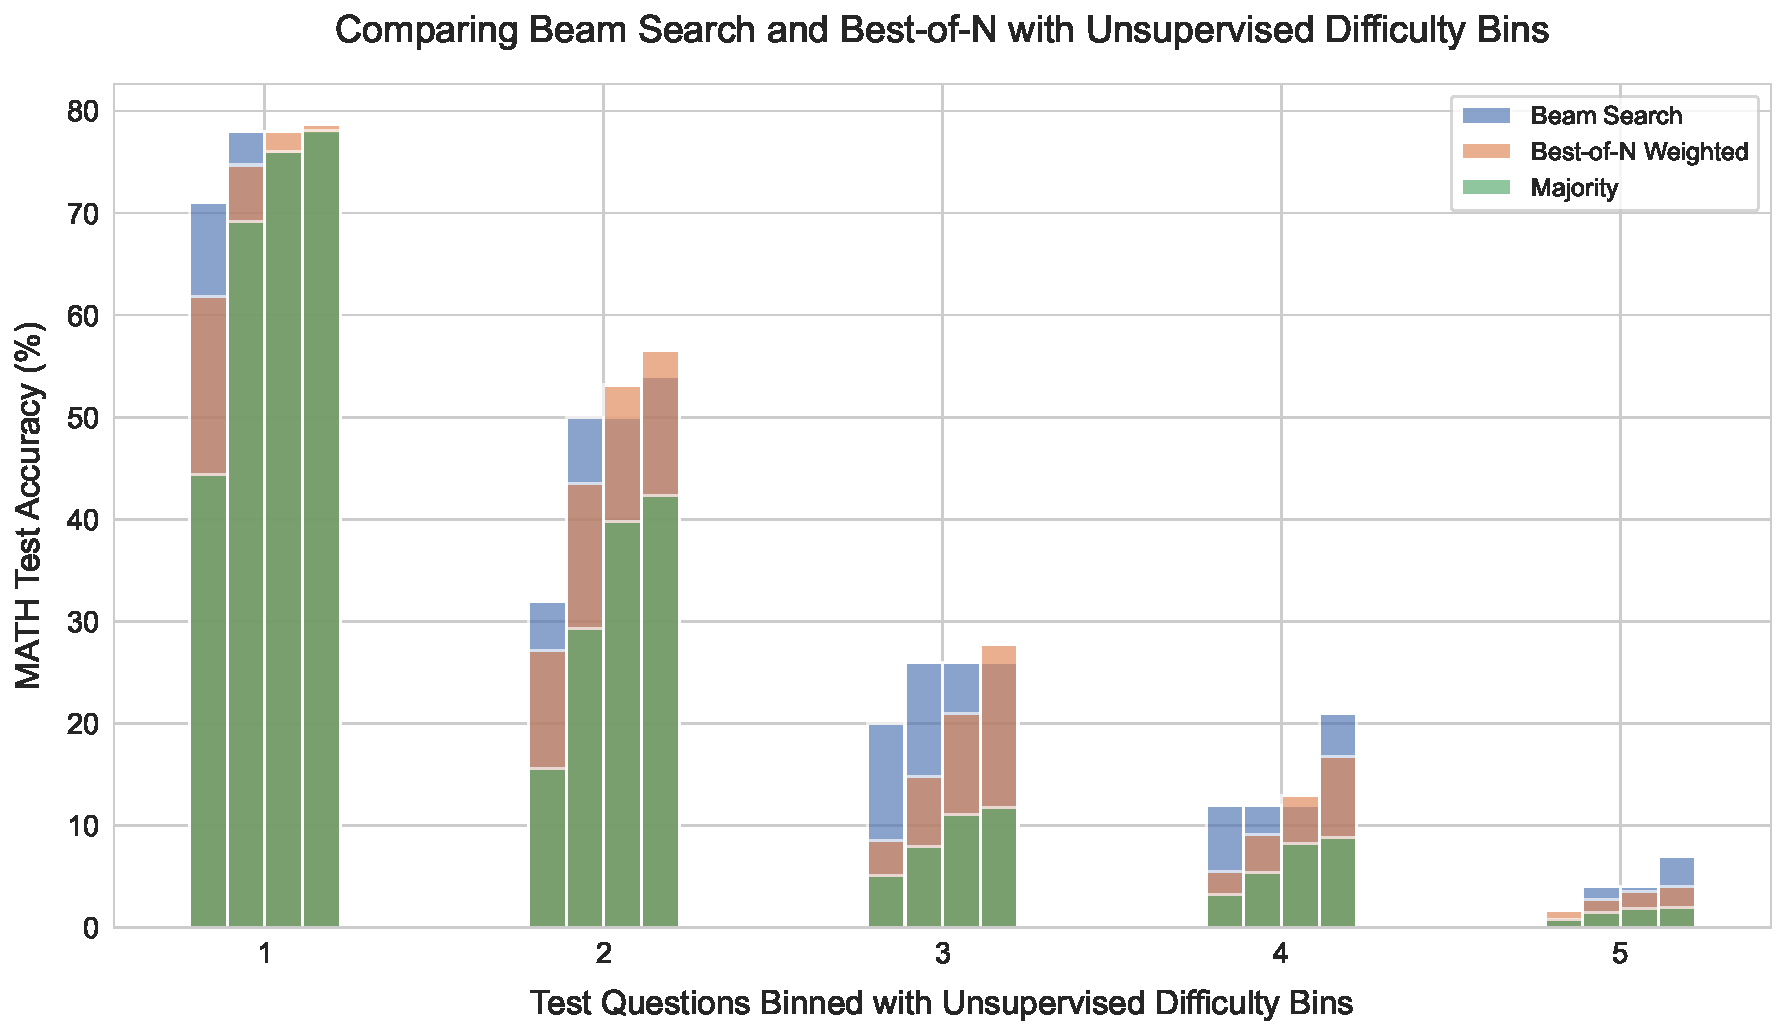
\includegraphics[width=.7\linewidth]{../papers/translations/testcompute/figures/search_unsup_difficulty_output.pdf}
\caption{原图 12: 用 PaLM 2-S* PRM, 在没有真实正确性信息时, 为 PRM 搜索计算难度分箱. 表现趋势与图\ref{testcompute-fig:comparing_search_and_beam_difficulty}的真实信息分箱基本相似. }
\label{testcompute-fig:search_unsupervised_difficulty}
\end{figure}

\originalsection{附录 D PRM 训练细节}
\paperlabel{D}{testcompute-app:prm_training}
将 PRM 微调为二分类器, 在解答每个步骤预测 $0$ 到 $1$ 的值. 以蒙特卡洛续采样得到的软值训练, 使用二元交叉熵损失, 例如 $-(y\log(\hat y)+(1-y)\log(1-\hat y))$, 其中 $y$ 为软真实值, $\hat y$ 为模型预测值. 用 AdamW 微调基础模型, 学习率 $3\times10^{-5}$, 批大小 $128$, dropout $0.05$, Adam 的 beta 为 $(0.9,0.95)$. 实施早停, 在随机保留的验证集上, 选择验证损失最低的检查点; 该验证集占原 PRM800k 训练划分问题的 $10\%$. 

PRM 微调时, 每题使用对应少样本提示基础模型产生的 $16$ 个样本. 每一步用同一基础模型、同一提示做 $16$ 次蒙特卡洛续采样, 估计步骤价值. 过滤所有未能输出有效、可解析最终答案的训练样本, 因为初步实验发现它们损害 PRM 表现. 

生成样本时, 如 Lightman 等人\cite{testcompute-lightman2023lets}, 提示基础模型以按换行分隔的逐步格式输出答案, 再用简单的换行切分将答案分成步骤. 提示细节见附录\ref{testcompute-app:prompting}. 

\originalsection{附录 E PRM 聚合策略比较}
\paperlabel{E}{testcompute-app:comparing_prm_agg}
比较将逐步 PRM 得分聚合为整个解答最终得分的不同方法: 1）如 Lightman 等人\cite{testcompute-lightman2023lets}, 取全部步骤得分最小值（“min”）; 2）将全部步骤正确性概率相乘（“prod”）; 3）仅取最后一步预测（“last”）. 图\ref{testcompute-fig:comparing_prm_aggregations}中, 最后一步优于另两种. 以往工作\cite{testcompute-lightman2023lets,testcompute-wang2023mathshepherd}发现 min 最好. 我们认为差异源于验证器使用软蒙特卡洛回报标签训练, 呈现方式与二元正确性标签很不同, 因此其他聚合策略可能不具有相同效果. 

有趣的是, 采用最后一步聚合时, 实际上将 PRM 当成 ORM 使用. 但 PRM 仍优于 ORM, 提示本设置中逐步 PRM 训练可能主要作为表示学习有用, 而不只是推理时的工具. 未来应进一步探索这一思路. 
\begin{figure}[htbp]
\centering
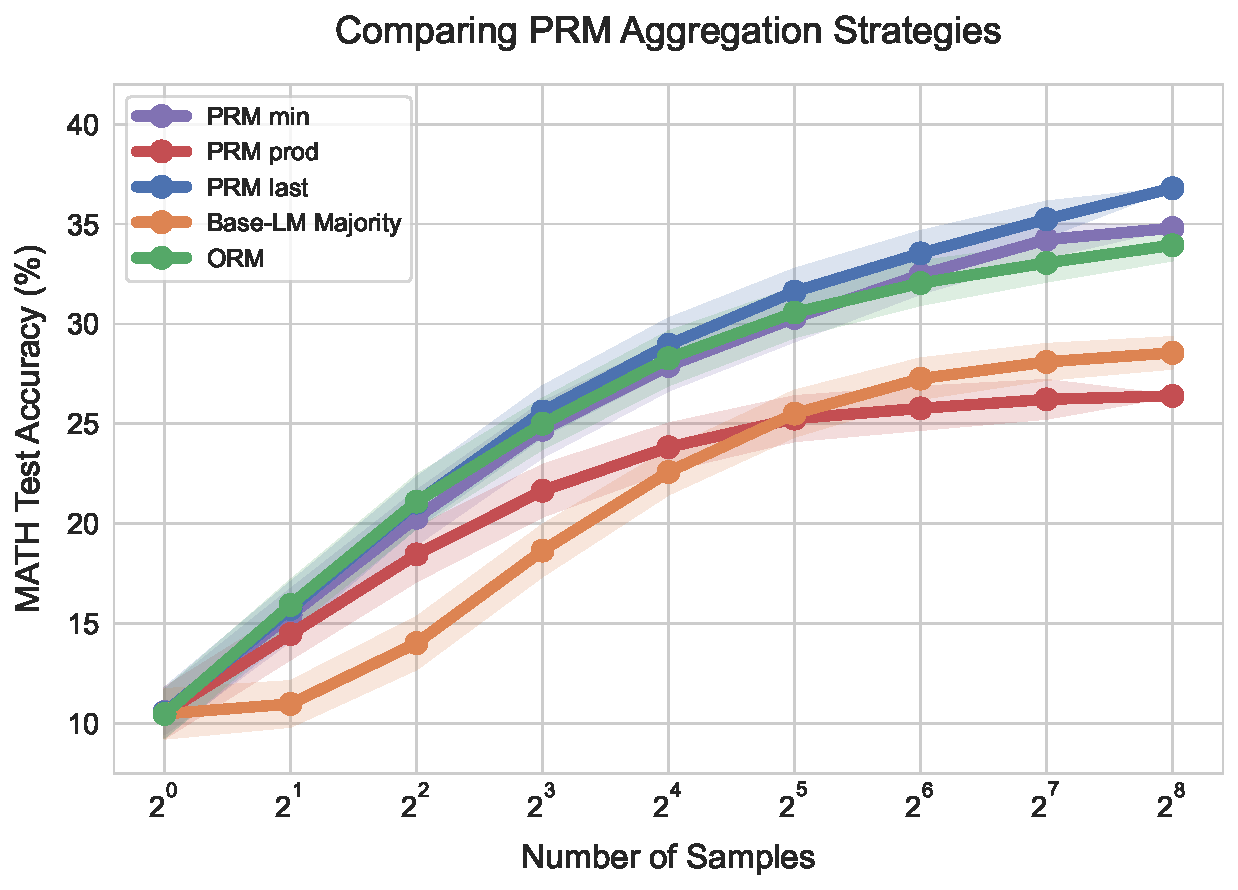
\includegraphics[width=.7\linewidth]{../papers/translations/testcompute/figures/prm_agg_comparing_output.pdf}
\caption{原图 13: 将逐步 PRM 得分聚合为完整解答最终得分的方法. “min”为各步骤最小得分, “prod”为各步骤正确性概率乘积, “last”为最后一步得分. last 在全部聚合策略中最好. }
\label{testcompute-fig:comparing_prm_aggregations}
\end{figure}

\originalsection{附录 F PRM 与 ORM 比较}
\paperlabel{F}{testcompute-app:comparing_prm_orm}
我们以 PaLM 2-S* 基础语言模型训练了 PRM 与 ORM. 图\ref{testcompute-fig:prm_v_orm}显示, PRM 超过 ORM, 差距随样本数量增加而扩大. 按附录\ref{testcompute-app:comparing_prm_agg}的方法, 用 PRM 最后一步预测给答案评分. 
\begin{figure}[htbp]
\centering
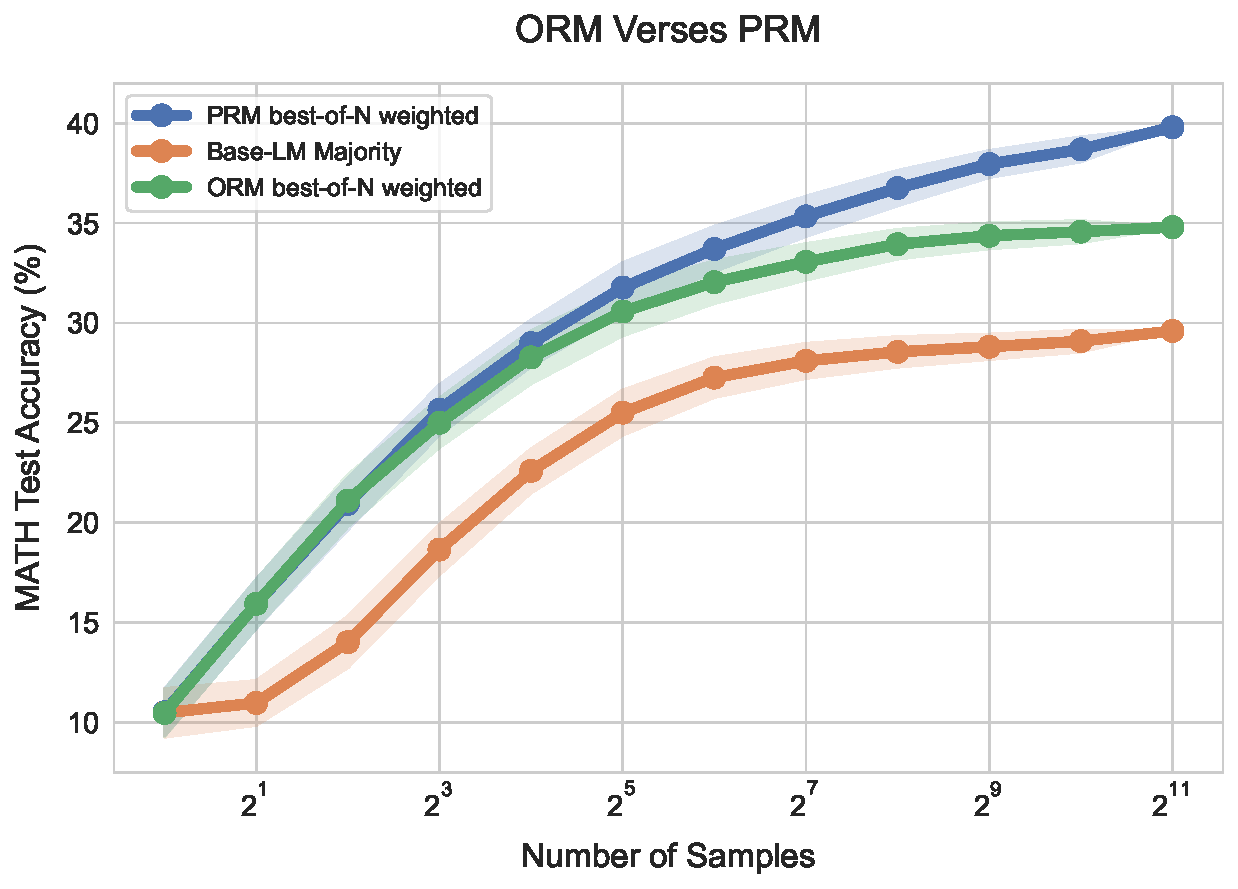
\includegraphics[width=.7\linewidth]{../papers/translations/testcompute/figures/prm_comparing_output3.pdf}
\caption{原图 14: 在 best-of-N 评估中, 比较从 PaLM 2-S* 微调的 PRM 与 ORM. 使用少样本提示的 PaLM 2-S* 基础语言模型采样输出. 样本较多时, PRM 大幅超过 ORM. }
\label{testcompute-fig:prm_v_orm}
\end{figure}

\originalsection{附录 G 提示细节}
\paperlabel{G}{testcompute-app:prompting}
为使基础模型以可应用 PRM 的逐步格式输出答案, 使用四样本提示, 其中示例随机选自 Lightman 等人\cite{testcompute-lightman2023lets}发布的 PRM800k 数据的正确答案. 具体使用 phase 1 训练划分中的答案, 即 GPT-4 生成、具有正确逐步格式的正确答案示例. 初步实验发现, 这种提示过程产生的结果类似 Lewkowycz 等人\cite{testcompute-lewkowycz2022solving}的提示. 我们用它为 PRM 和修订模型生成训练数据, 也用它在测试集上依据 PRM 搜索. 评判此提示预测的最终答案时, 使用 Lightman 等人\cite{testcompute-lightman2023lets}发布的评分函数. 
\begin{remark}
译者注: 该版本仅说明四样本提示的来源与选取方式, 并未刊出四个示例的逐字提示字符串; 译本也不补造提示词. 
\end{remark}

\originalsection{附录 H 修订模型微调细节}
\paperlabel{H}{testcompute-app:revision_finetune}
按第\ref{testcompute-sec:revision_setup}节流程微调修订模型. 先每题采样 $64$ 个输出, 过滤以无效解答结束的答案. 对每个正确答案, 从 $0$--$4$ 均匀采样一个数, 表示训练上下文包含多少错误答案. 正确答案用作轨迹的最后一个答案（训练模型生成它）, 错误答案放入上下文. 若采样数大于 $0$, 按字符级编辑距离找到最接近的错误答案, 将它作为轨迹中最后一个错误答案; 目的是选择与正确答案具有一定相关性的错误答案, 改善学习. 其余错误答案从可用答案集合随机抽取. 若采样得到的错误答案不足四个, 则截断均匀分布的上界, 使其匹配错误样本数量. 用此流程为全部训练问题生成轨迹. 

随后在生成轨迹中的正确答案解答上微调基础语言模型. 用 AdamW, 学习率 $10^{-5}$, 批大小 $128$, dropout $0.0$, Adam beta 为 $(0.9,0.95)$. 

通常, 在按上述方法生成轨迹的评估集上测损失, 不能提供良好早停信号. 相反, 评估损失开始上升很久之后的检查点, 修订能力要强得多. 可能因为微调修订模型后, 评估集成了异策略数据, 相对于模型自身同策略生成的轨迹, 自然分布外. 因此, 选择稍晚于验证集出现过拟合时点的修订模型检查点. 

\originalsection{附录 I 修订模型选择标准}
\paperlabel{I}{testcompute-app:revision_selection}
如第\ref{testcompute-sec:revision_setup}节, 为有效使用修订模型, 需要标准来选择一条轨迹内部及多条并行轨迹之间的最佳答案. 使用两种方法: 1）ORM 验证器; 2）多数投票. 

ORM 按附录\ref{testcompute-app:revision_verifier}流程, 在修订模型输出上训练. 推理时用它选择最佳答案. 由于聚合有两个维度（每条修订轨迹内、多条轨迹间）, 采用层次策略: 先在各轨迹内选择, 再跨轨迹聚合这些答案. 轨迹内部先执行加权 best-of-N, 得到得分最高的最终答案, 再选择具有这一加权 best-of-N 最优最终答案的最高分解答. 跨修订链选择时, 用每条链的最佳答案, 再执行一次加权 best-of-N; 第二轮所得答案为最终预测. 

多数投票时, 若轨迹太短或轨迹太少, 层次聚合会出问题, 因为样本不足时多数投票无法有效选择最佳选项. 因此, 对所有轨迹中的全部答案一起投票, 取多数作为最终答案. 相比层次方法, 这带来平滑得多的扩展行为. 

\originalsection{附录 J 修订模型验证器训练}
\paperlabel{J}{testcompute-app:revision_verifier}
在 PaLM 2-S* 基础模型输出上微调的 PRM, 用于 PaLM 2-S* 修订模型输出时, 效果较差（见图\ref{testcompute-fig:revision_verifier_ablations}左）, 可能源于修订模型的分布偏移. 因此, 为修订模型单独训练 ORM 验证器. 也可以训练 PRM, 但逐步标签生成成本高, 因而选 ORM. 

对标准 ORM 作了少量适配: 微调时将先前修订置于上下文, 让验证器获得与修订模型相同的上下文, 为当前答案评分时能看到之前的尝试. 其他实验细节与 PRM 训练相同. 

经验上, 上下文包含修订历史会略微改善表现（见图\ref{testcompute-fig:revision_verifier_ablations}右）. 即使不包含修订, 顺序修订也仍略胜于并行, 说明顺序采样的改进并不只是来自验证器上下文. 
\begin{figure}[htbp]
\centering
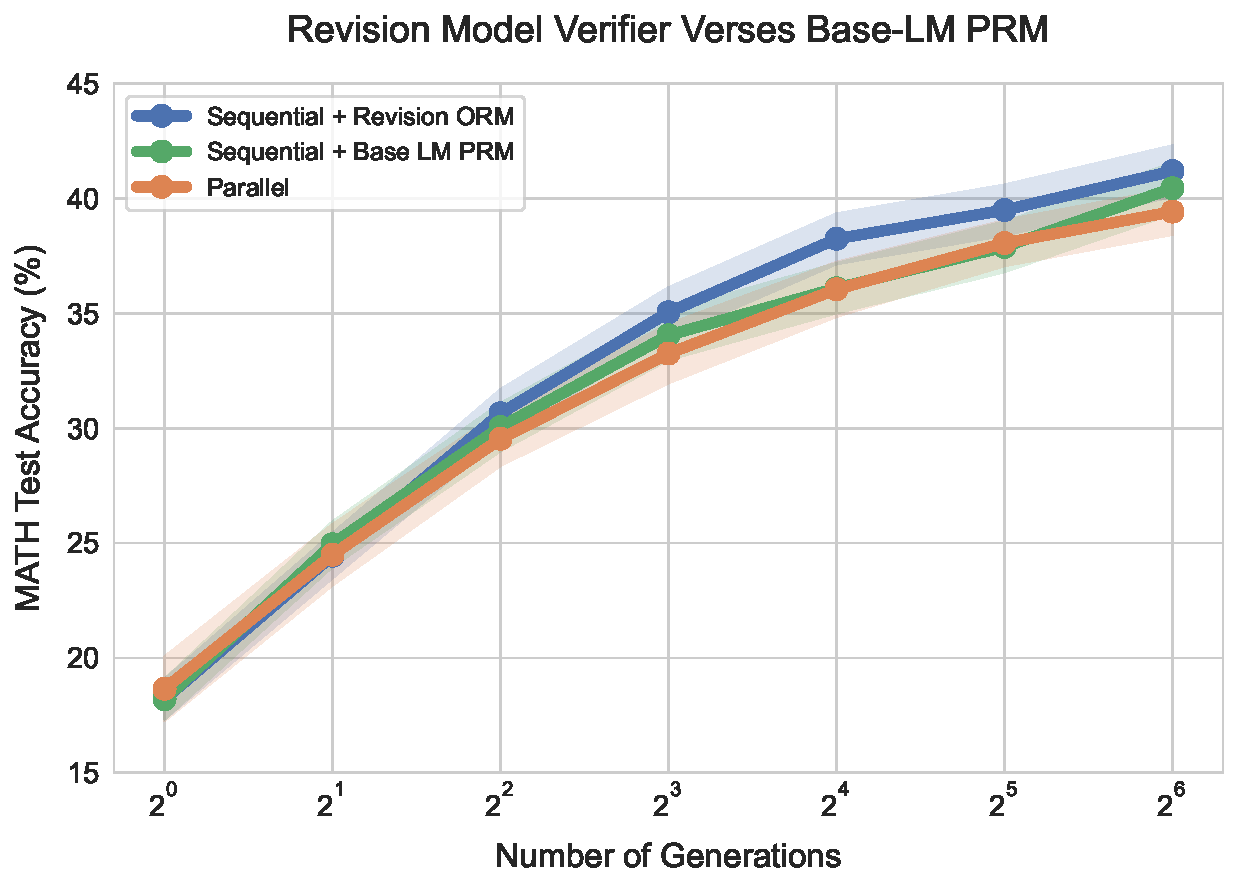
\includegraphics[width=.49\linewidth]{../papers/translations/testcompute/figures/revision_model_with_prm_verses_revision_orm_output.pdf}
\label{testcompute-fig:revision_verifier_v_prm}
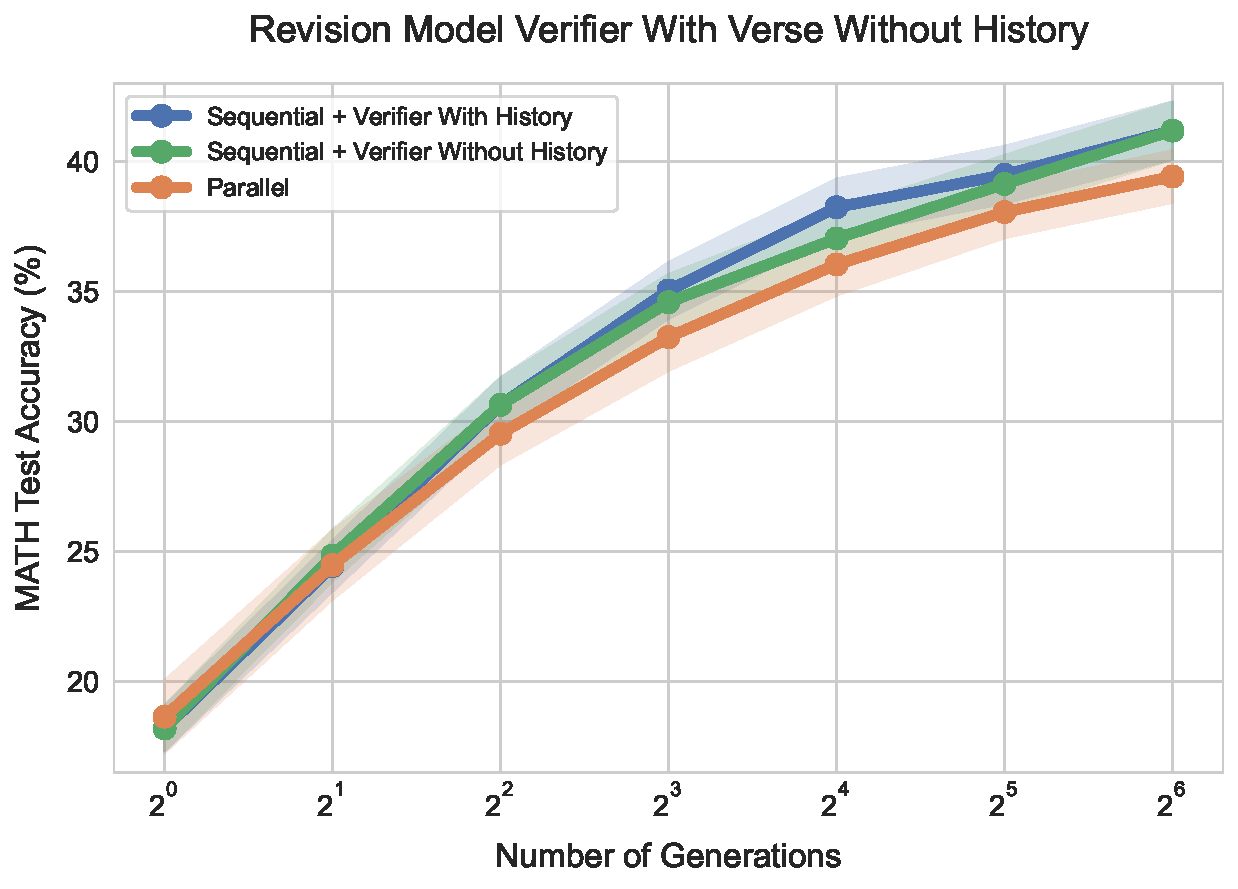
\includegraphics[width=.49\linewidth]{../papers/translations/testcompute/figures/revision_model_with_without_history_output.pdf}
\label{testcompute-fig:revision_verifier_w_v_wo_history}
\caption{原图 15. \textbf{左: }比较修订模型输出上训练的 ORM, 与 PaLM 2-S* 基础模型输出上训练的 PRM. 对修订模型输出, 适配它的 ORM 更好, 可能由于分布偏移. \textbf{右: }消融先前修订进入验证器上下文的影响. 包含修订略有帮助, 但两种设置都超过并行基线. }
\label{testcompute-fig:revision_verifier_ablations}
\end{figure}

\originalsection{附录 K ReST-EM 修订模型实验}
\paperlabel{K}{testcompute-app:rest_revision_model}
我们尝试用简化的强化学习算法 $\text{ReST}^{\text{EM}}$\cite{testcompute-singh2024human}进一步优化 PaLM 2-S* 修订模型. 具体而言, 对 MATH 训练集每题生成 $64$ 条最长为 $5$ 的修订轨迹, 在每条轨迹第一个正确答案处停止. 然后用生成数据中的正确答案微调基础语言模型. 为帮助模型学习任务, 显式平衡轨迹长度分布. 

图\ref{testcompute-fig:rest_em_revisions}显示新模型在改变顺序与并行比例时的表现. 额外顺序修订大幅损害这一新模型的表现. 我们推测, 这是因为运行 $\text{ReST}^{\text{EM}}$ 得到的在线数据加剧修订数据的虚假相关性, 使优化后的模型无法学会修订任务. 我们认为, 类似 Qu 等人\cite{testcompute-qu2024recursive}的更离线数据收集策略可能更有效, 进一步探索留待未来. 
\begin{figure}[htbp]
\centering
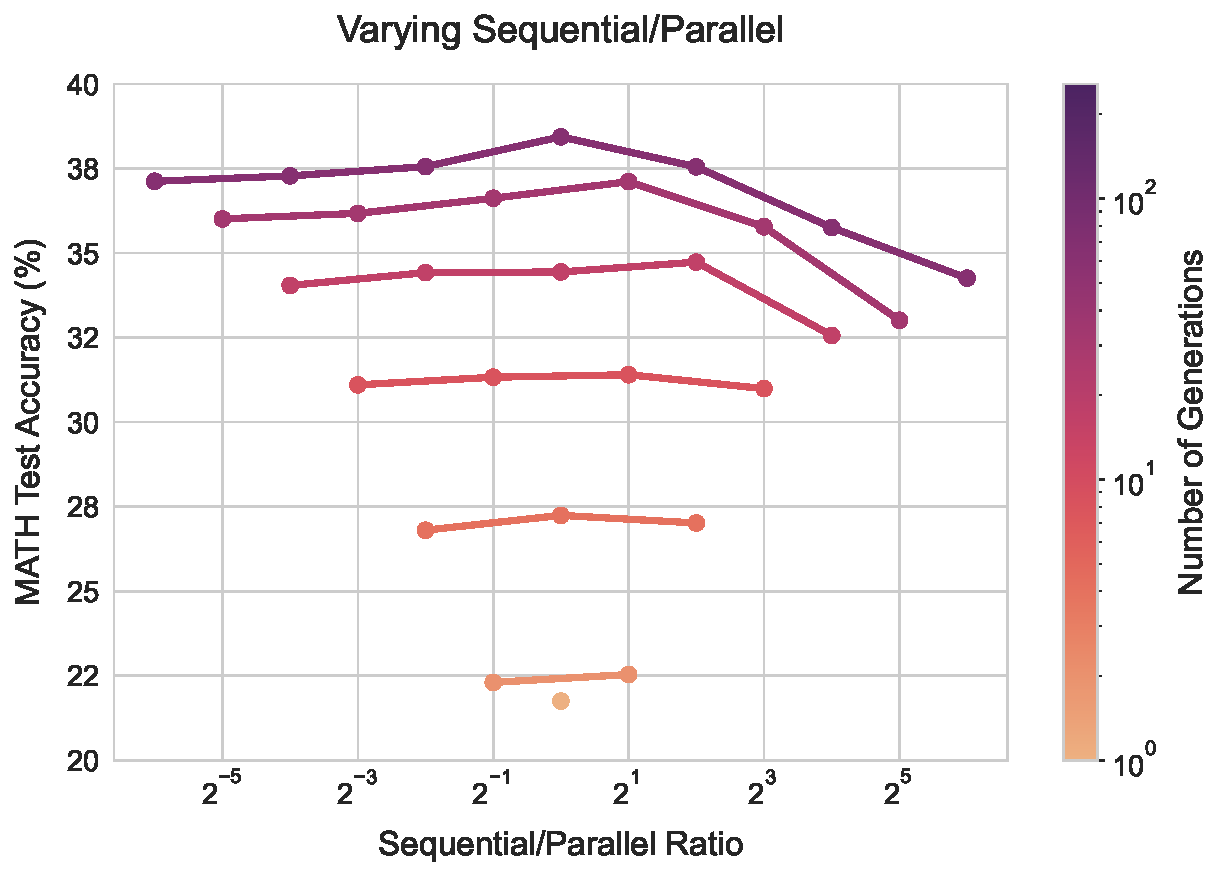
\includegraphics[width=.7\linewidth]{../papers/translations/testcompute/figures/rest_em_revision_model_iso_gens_output.pdf}
\caption{原图 16: 改变顺序与并行比例时, $\text{ReST}^{\text{EM}}$ 优化修订模型的表现. 用多数投票选择答案. 增加顺序修订后, 这一优化模型表现显著下降. }
\label{testcompute-fig:rest_em_revisions}
\end{figure}

\originalsection{附录 L 修订模型输出实例}
\paperlabel{L}{testcompute-app:revision_example_outputs}
图\ref{testcompute-fig:revisions_ex1}、\ref{testcompute-fig:revisions_ex2}、\ref{testcompute-fig:revisions_ex3}、\ref{testcompute-fig:revisions_ex4}、\ref{testcompute-fig:revisions_ex5}、\ref{testcompute-fig:revisions_ex6}、\ref{testcompute-fig:revisions_ex7}给出精选的修订模型输出. 
\begin{remark}
译者说明: 以下保留原截图, 并逐句提供其中题目与模型输出的中文转写. 绿色、红色由原图标示; 这些是论文所展示的模型作答, 并非译者给出的正确解答. 原有算术错误、推理错误、重复语句、尝试编号和最终答案标记均保留. 截图中以字面 LaTeX 字符串显示的公式, 在中文转写中排为数学式; 不改变数值与运算. 转写中的“我们”属于模型原输出. 
\end{remark}

\begin{figure}[htbp]
\centering
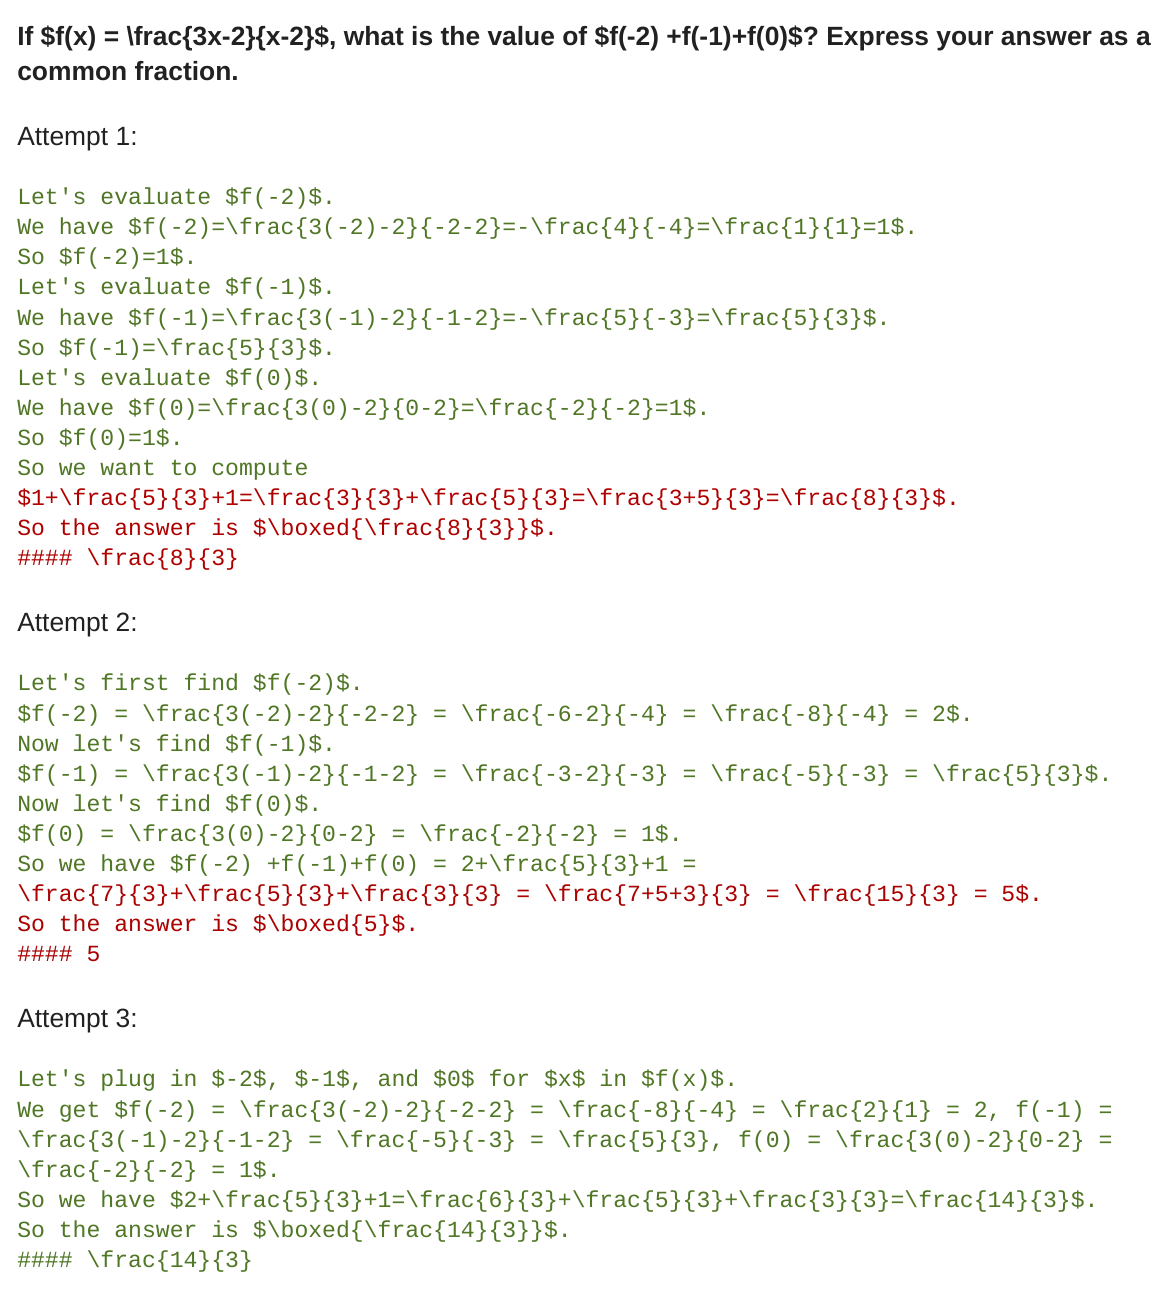
\includegraphics[width=.97\linewidth,height=.72\textheight,keepaspectratio]{../papers/translations/testcompute/figures/revisions_ex1.png}
\caption{原图 17: 修订模型实例 1. 前两次尝试末尾求和错误, 第三次成功, 得到正确答案. }
\label{testcompute-fig:revisions_ex1}
\end{figure}
\subsection*{原图 17 的中文转写}
\label{testcompute-image-text:revisions_ex1}
\textbf{题目: }若 $f(x)=\frac{3x-2}{x-2}$, 求 $f(-2)+f(-1)+f(0)$. 答案写为普通分数. 

\textbf{尝试 1: }来计算 $f(-2)$. 有 $f(-2)=\frac{3(-2)-2}{-2-2}=-\frac4{-4}=\frac11=1$. 所以 $f(-2)=1$. 来计算 $f(-1)$. 有 $f(-1)=\frac{3(-1)-2}{-1-2}=-\frac5{-3}=\frac53$. 所以 $f(-1)=\frac53$. 来计算 $f(0)$. 有 $f(0)=\frac{3(0)-2}{0-2}=\frac{-2}{-2}=1$. 所以 $f(0)=1$. 因此我们要计算 $1+\frac53+1=\frac33+\frac53=\frac{3+5}3=\frac83$. 所以答案为 $\boxed{\frac83}$. \texttt{\#\#\#\#} $\frac83$. 

\textbf{尝试 2: }先求 $f(-2)$. $f(-2)=\frac{3(-2)-2}{-2-2}=\frac{-6-2}{-4}=\frac{-8}{-4}=2$. 现在求 $f(-1)$. $f(-1)=\frac{3(-1)-2}{-1-2}=\frac{-3-2}{-3}=\frac{-5}{-3}=\frac53$. 现在求 $f(0)$. $f(0)=\frac{3(0)-2}{0-2}=\frac{-2}{-2}=1$. 于是有 $f(-2)+f(-1)+f(0)=2+\frac53+1=\frac73+\frac53+\frac33=\frac{7+5+3}3=\frac{15}3=5$. 所以答案为 $\boxed5$. \texttt{\#\#\#\#} $5$. 

\textbf{尝试 3: }在 $f(x)$ 中用 $-2$、$-1$、$0$ 代入 $x$. 得到 $f(-2)=\frac{3(-2)-2}{-2-2}=\frac{-8}{-4}=\frac21=2$, $f(-1)=\frac{3(-1)-2}{-1-2}=\frac{-5}{-3}=\frac53$, $f(0)=\frac{3(0)-2}{0-2}=\frac{-2}{-2}=1$. 因此 $2+\frac53+1=\frac63+\frac53+\frac33=\frac{14}3$. 所以答案为 $\boxed{\frac{14}3}$. \texttt{\#\#\#\#} $\frac{14}3$. 

\begin{figure}[htbp]
\centering
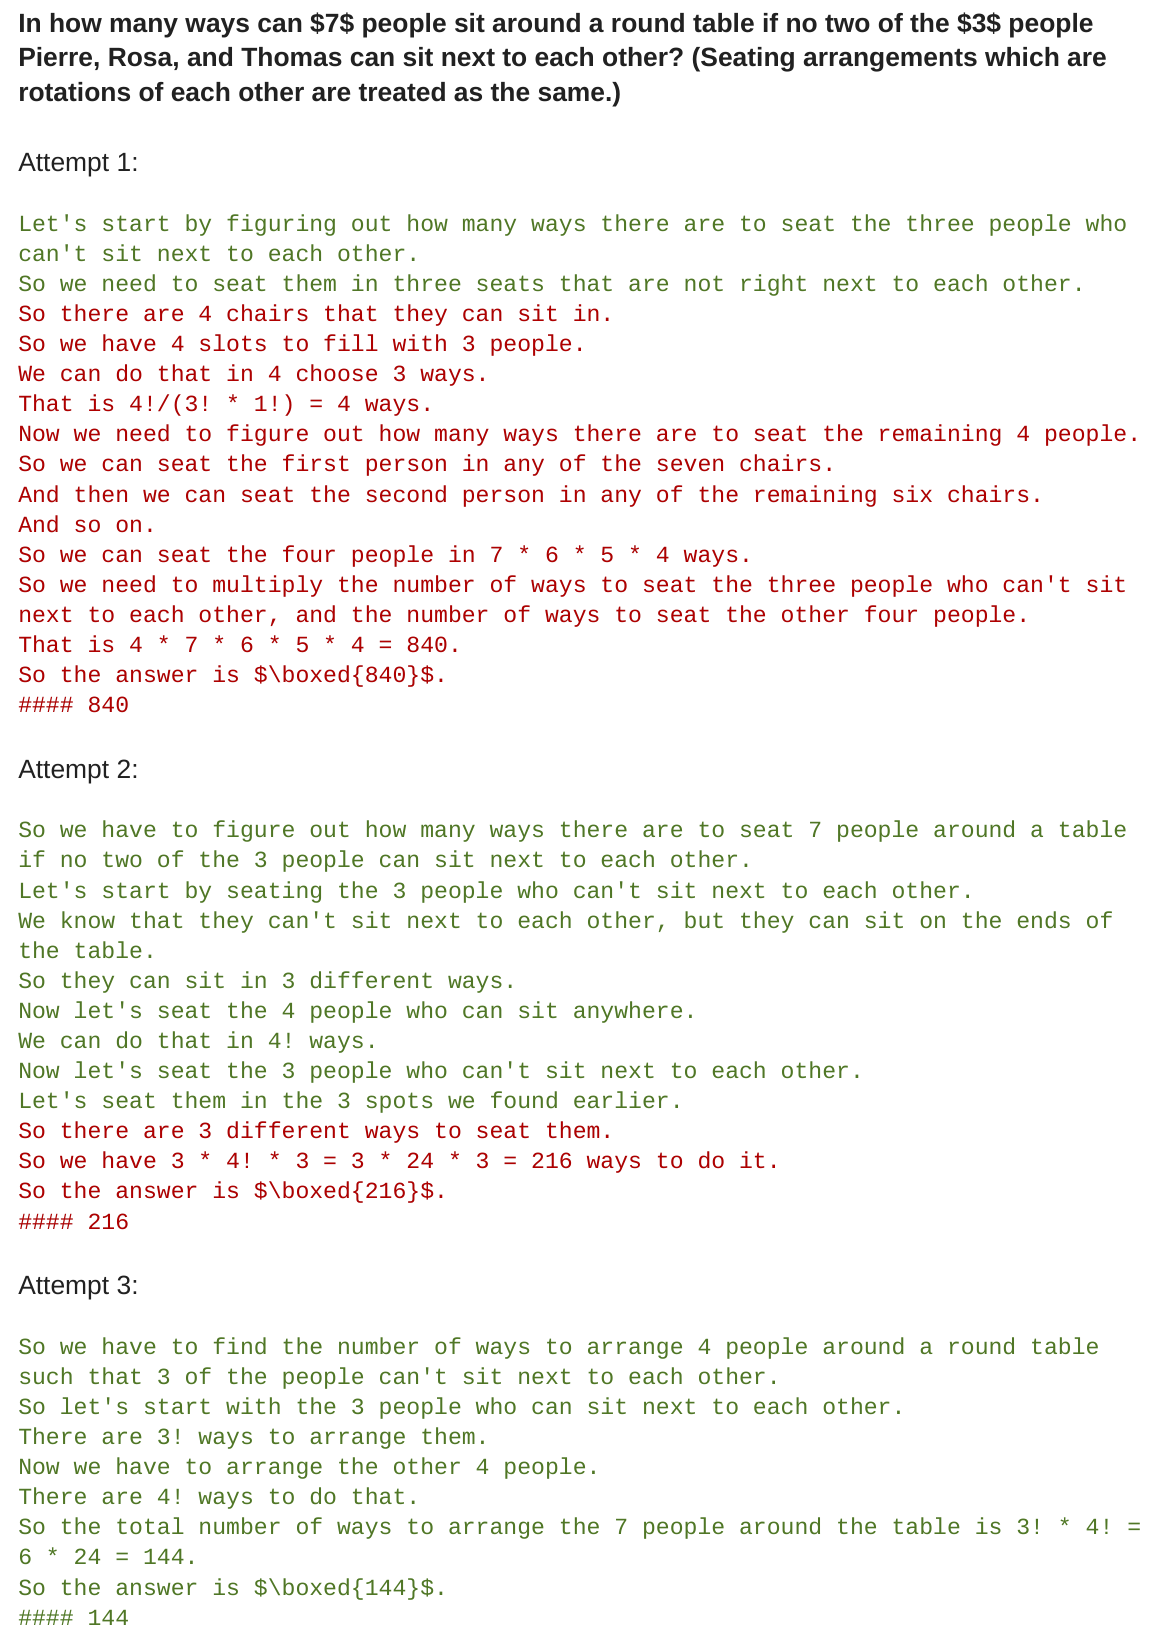
\includegraphics[width=.97\linewidth,height=.72\textheight,keepaspectratio]{../papers/translations/testcompute/figures/revisions_ex2.png}
\caption{原图 18: 修订模型实例 2. 首次采用错误方法, 第二次更接近但末尾出错, 最后一次得到正确答案. }
\label{testcompute-fig:revisions_ex2}
\end{figure}
\subsection*{原图 18 的中文转写}
\label{testcompute-image-text:revisions_ex2}
\textbf{题目: }七个人围坐圆桌, 若 Pierre、Rosa、Thomas 三人任意两人不能相邻, 有多少坐法? 旋转后相同的安排视为同一种. 

\textbf{尝试 1: }先算不能相邻的三人有多少坐法. 因此要把他们安排在三个不紧挨的座位上. 所以有四张椅子可坐. 因此有四个位置让三人填. 可以有 $\binom43$ 种, 也就是 $4!/(3!\times1!)=4$ 种. 现在算其余四人多少坐法. 第一个人可坐七张椅子中的任一张, 第二个可坐余下六张任一张, 依此类推. 因此四人可有 $7\times6\times5\times4$ 种坐法. 把不能相邻三人的坐法数与其余四人的坐法数相乘, 即 $4\times7\times6\times5\times4=840$. 答案为 $\boxed{840}$. \texttt{\#\#\#\#} $840$. 

\textbf{尝试 2: }要算七个人围坐圆桌、三人任意两人不能相邻的坐法. 先安排不能相邻的三人. 他们不能相邻, 但可以坐桌子的两端. 因此有三种坐法. 现在安排可任意坐的四人, 有 $4!$ 种. 现在再安排不能相邻的三人, 坐在刚才找到的三个位置上. 因此有三种坐法. 于是总共 $3\times4!\times3=3\times24\times3=216$ 种. 答案为 $\boxed{216}$. \texttt{\#\#\#\#} $216$. 

\textbf{尝试 3: }要算四个人围坐圆桌、其中三人不能相邻的安排数. 先看可以相邻的三人, 有 $3!$ 种排列. 现在安排另外四人, 有 $4!$ 种. 所以七人围桌总排列数为 $3!\times4!=6\times24=144$. 答案为 $\boxed{144}$. \texttt{\#\#\#\#} $144$. 

\begin{figure}[htbp]
\centering
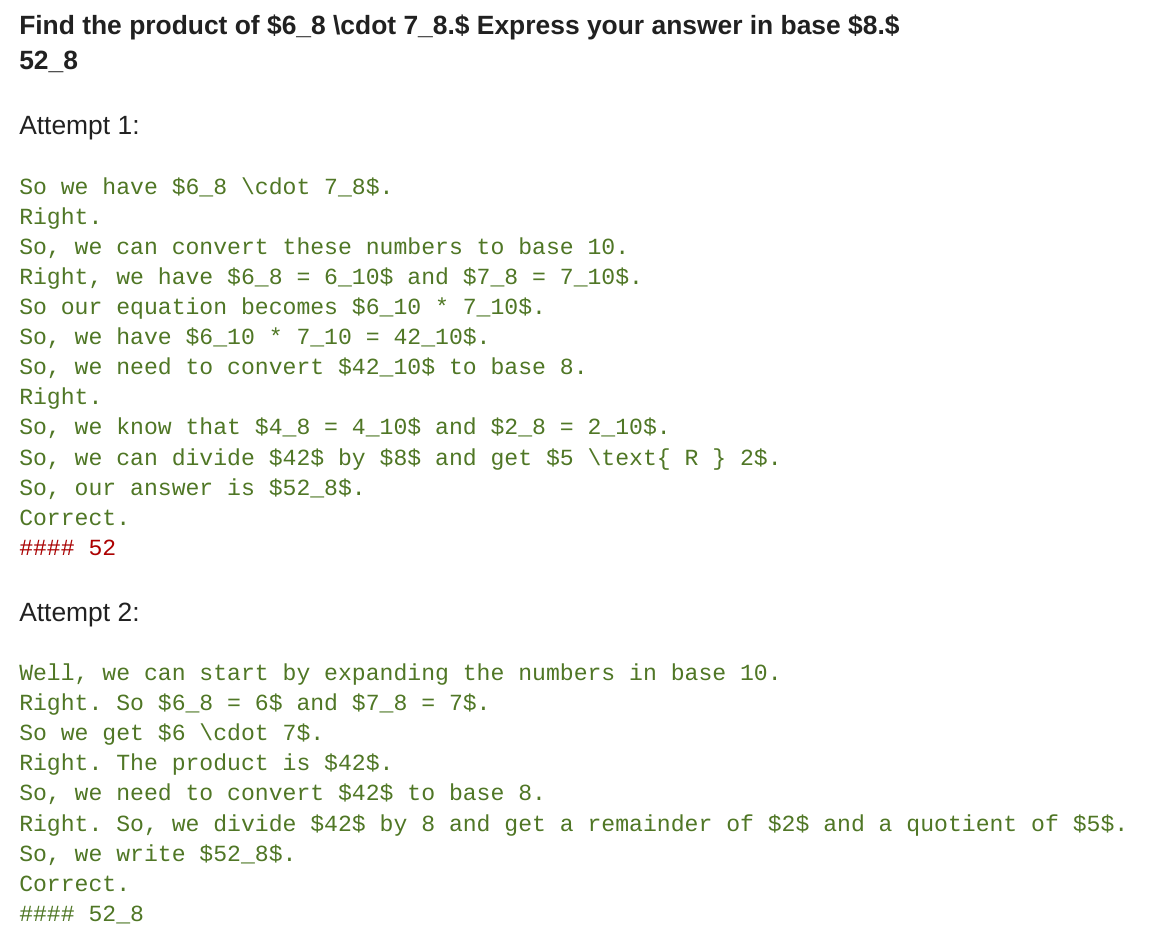
\includegraphics[width=.97\linewidth,height=.72\textheight,keepaspectratio]{../papers/translations/testcompute/figures/revisions_ex3.png}
\caption{原图 19: 修订模型实例 3. 首次最终答案的格式错误, 第二次纠正了格式. }
\label{testcompute-fig:revisions_ex3}
\end{figure}
\subsection*{原图 19 的中文转写}
\label{testcompute-image-text:revisions_ex3}
\textbf{题目: }求 $6_8\cdot7_8$, 答案用八进制表示. 原图题下另列 $52_8$. 

\textbf{尝试 1: }有 $6_8\cdot7_8$. 对. 因此可以转成十进制. 对, 有 $6_8=6_{10}$, $7_8=7_{10}$. 于是变为 $6_{10}\times7_{10}$. 有 $6_{10}\times7_{10}=42_{10}$. 需要把 $42_{10}$ 转成八进制. 对. 知道 $4_8=4_{10}$, $2_8=2_{10}$. 将 $42$ 除以 $8$ 得 $5$ 余 $2$. 所以答案为 $52_8$. 正确. \texttt{\#\#\#\#} $52$. 

\textbf{尝试 2: }可以先按十进制展开这些数. 对, $6_8=6$, $7_8=7$. 得到 $6\cdot7$. 对, 乘积为 $42$. 需要转成八进制. 对, 将 $42$ 除以 $8$, 余 $2$、商 $5$. 写作 $52_8$. 正确. \texttt{\#\#\#\#} $52_8$. 

\begin{figure}[htbp]
\centering
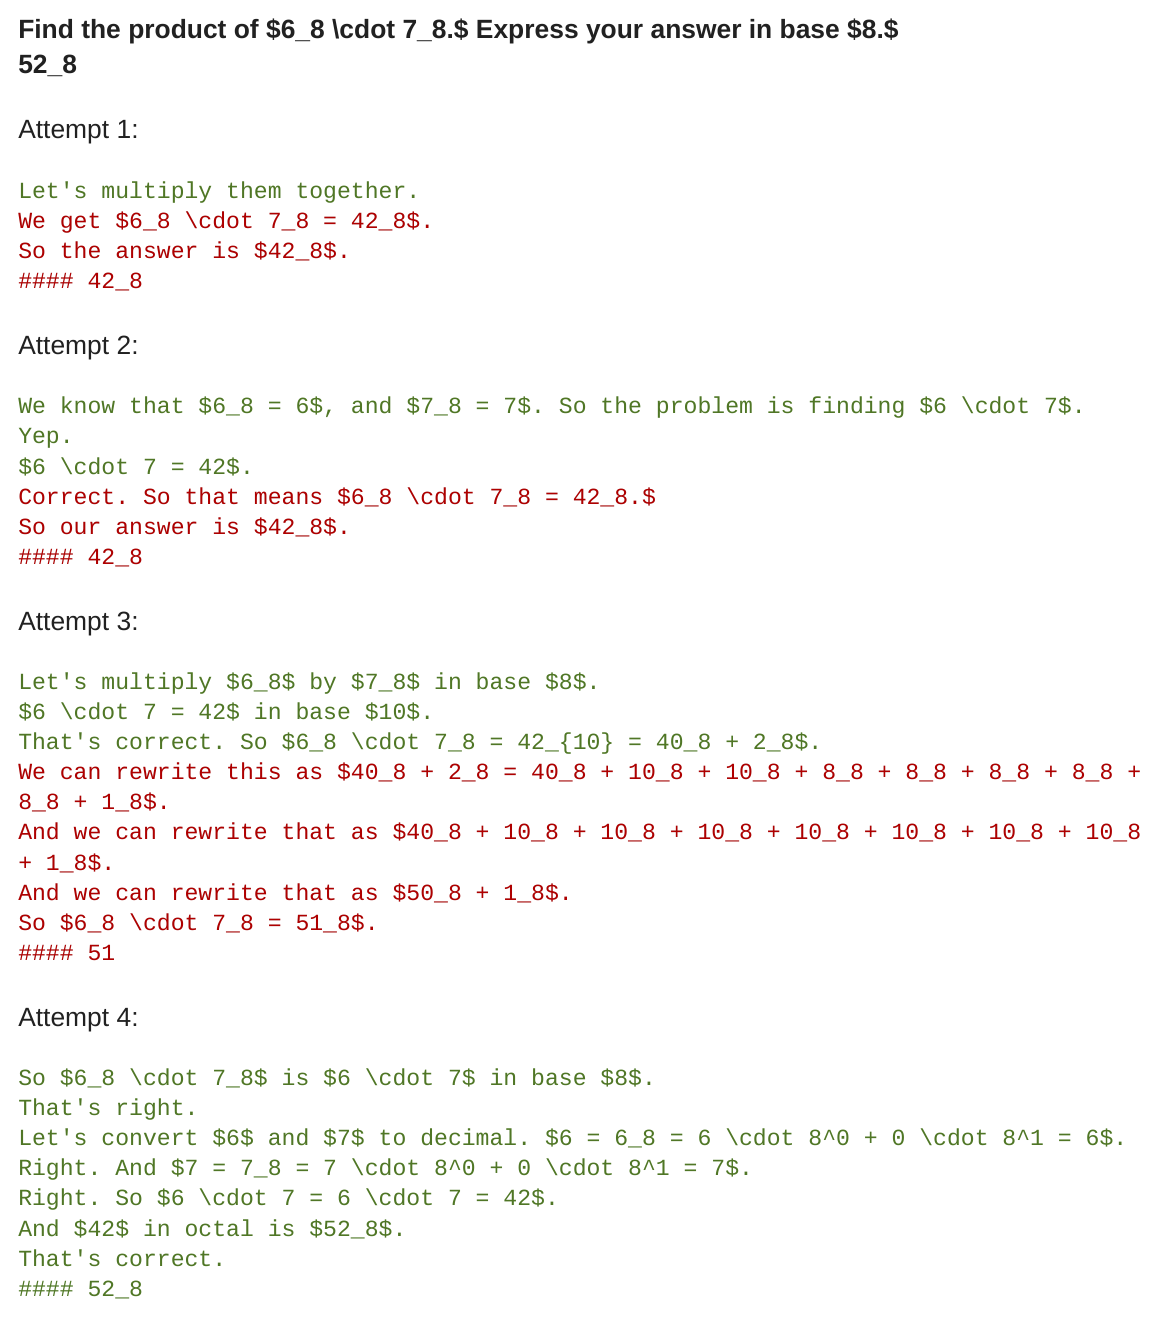
\includegraphics[width=.97\linewidth,height=.72\textheight,keepaspectratio]{../papers/translations/testcompute/figures/revisions_ex4.png}
\caption{原图 20: 修订模型实例 4. 前几次尝试从十进制转八进制失败, 最后一次计算正确. }
\label{testcompute-fig:revisions_ex4}
\end{figure}
\subsection*{原图 20 的中文转写}
\label{testcompute-image-text:revisions_ex4}
\textbf{题目: }求 $6_8\cdot7_8$, 答案用八进制表示. 原图题下另列 $52_8$. 

\textbf{尝试 1: }把它们相乘. 得到 $6_8\cdot7_8=42_8$. 所以答案为 $42_8$. \texttt{\#\#\#\#} $42_8$. 

\textbf{尝试 2: }知道 $6_8=6$, $7_8=7$, 因此求 $6\cdot7$. 是的. $6\cdot7=42$. 正确, 这意味着 $6_8\cdot7_8=42_8$. 答案为 $42_8$. \texttt{\#\#\#\#} $42_8$. 

\textbf{尝试 3: }用八进制将 $6_8$ 乘 $7_8$. 十进制下 $6\cdot7=42$. 正确, 所以 $6_8\cdot7_8=42_{10}=40_8+2_8$. 可改写为
\begin{align*}
40_8+2_8&=40_8+10_8+10_8+8_8+8_8+8_8+8_8+8_8+1_8.
\end{align*}
再改写为 $40_8+10_8+10_8+10_8+10_8+10_8+10_8+10_8+1_8$. 再改写为 $50_8+1_8$. 因此 $6_8\cdot7_8=51_8$. \texttt{\#\#\#\#} $51$. 

\textbf{尝试 4: }$6_8\cdot7_8$ 是八进制下的 $6\cdot7$. 对. 把 $6$、$7$ 转成十进制: $6=6_8=6\cdot8^0+0\cdot8^1=6$. 对, $7=7_8=7\cdot8^0+0\cdot8^1=7$. 对, 所以 $6\cdot7=6\cdot7=42$. 而 $42$ 的八进制为 $52_8$. 正确. \texttt{\#\#\#\#} $52_8$. 

\begin{figure}[htbp]
\centering
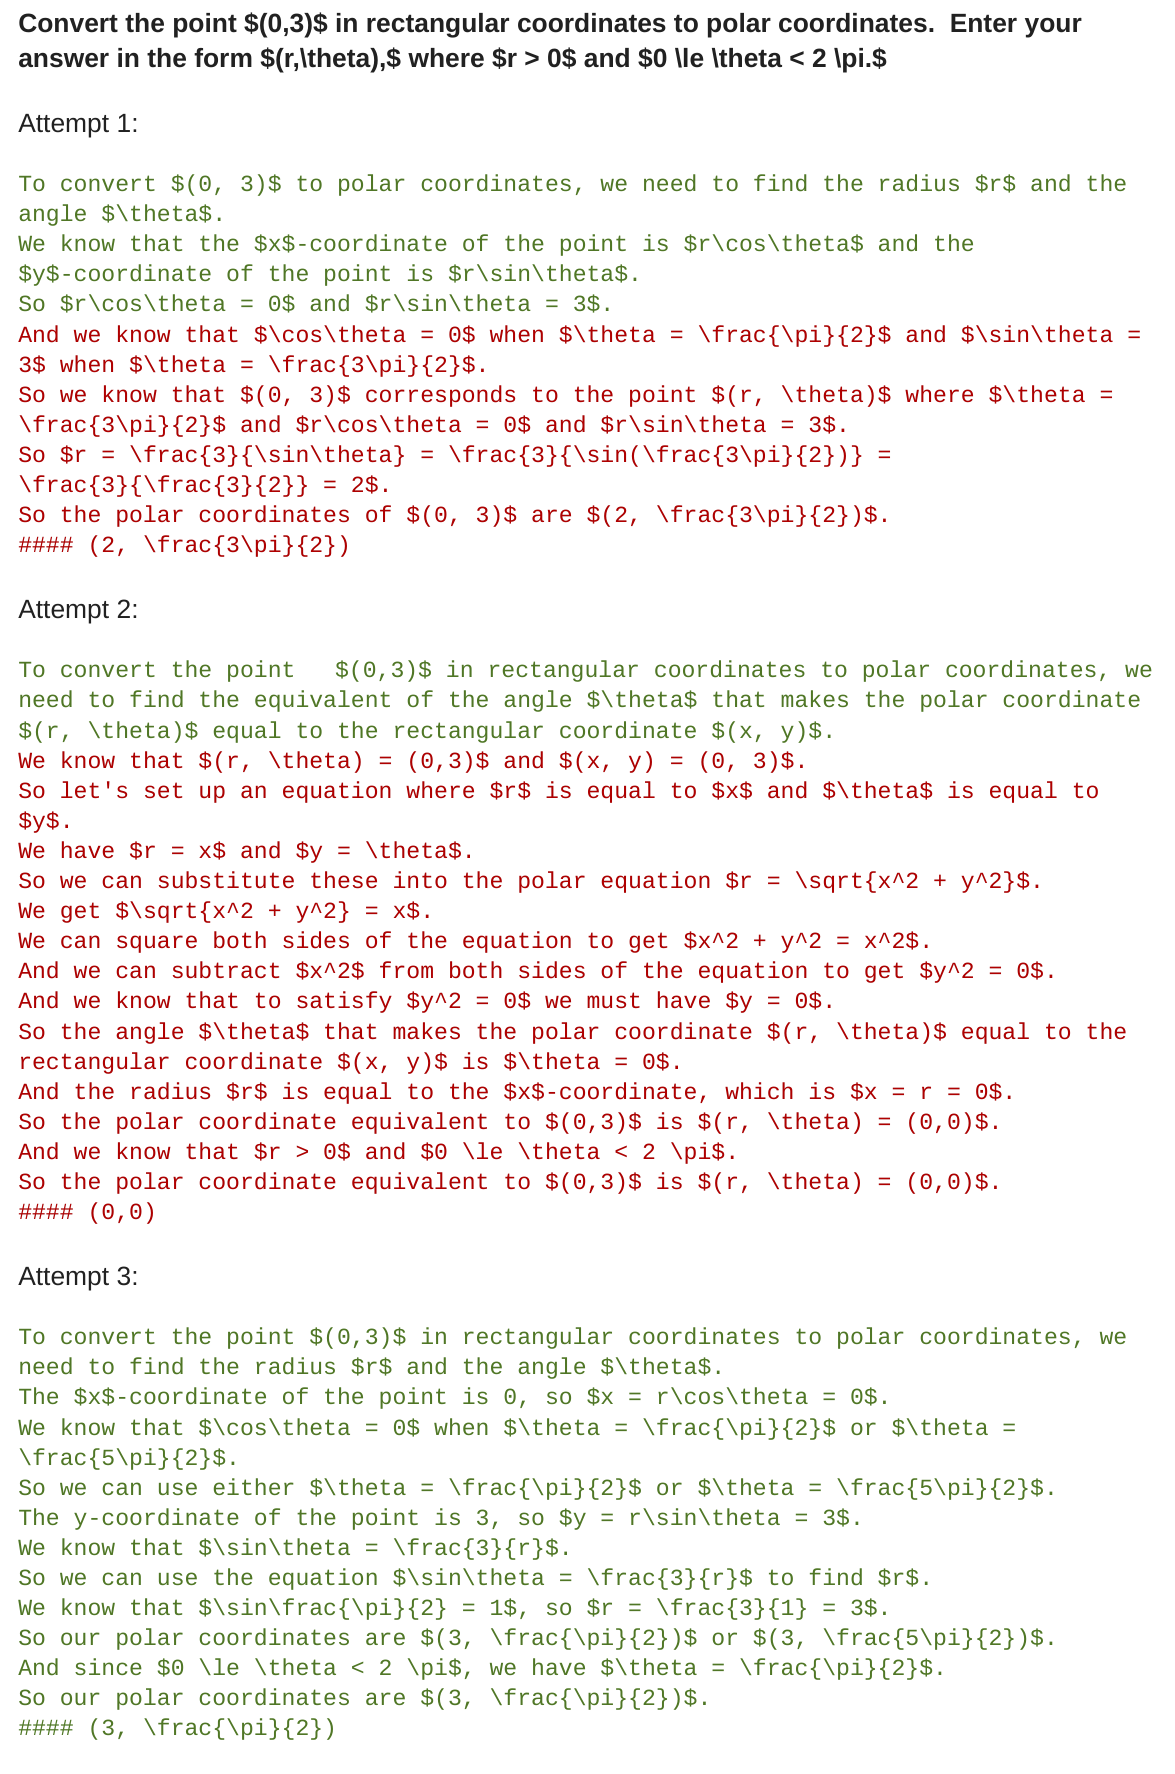
\includegraphics[width=.97\linewidth,height=.72\textheight,keepaspectratio]{../papers/translations/testcompute/figures/revisions_ex5.png}
\caption{原图 21: 修订模型实例 5. 前两次将欧氏坐标转成极坐标时出错, 最后一次没有这些错误. }
\label{testcompute-fig:revisions_ex5}
\end{figure}
\subsection*{原图 21 的中文转写}
\label{testcompute-image-text:revisions_ex5}
\textbf{题目: }将直角坐标 $(0,3)$ 转为极坐标, 答案写为 $(r,\theta)$, 其中 $r>0$, $0\le\theta<2\pi$. 

\textbf{尝试 1: }转换 $(0,3)$ 要求半径 $r$ 与角 $\theta$. 知道点的 $x$ 坐标为 $r\cos\theta$, $y$ 坐标为 $r\sin\theta$. 所以 $r\cos\theta=0$, $r\sin\theta=3$. 知道 $\theta=\pi/2$ 时 $\cos\theta=0$, $\theta=3\pi/2$ 时 $\sin\theta=3$. 所以 $(0,3)$ 对应 $(r,\theta)$, 其中 $\theta=3\pi/2$, 且 $r\cos\theta=0$, $r\sin\theta=3$. 所以 $r=\frac3{\sin\theta}=\frac3{\sin(3\pi/2)}=\frac3{3/2}=2$. 故极坐标为 $(2,3\pi/2)$. \texttt{\#\#\#\#} $(2,3\pi/2)$. 

\textbf{尝试 2: }将直角坐标 $(0,3)$ 转成极坐标, 需要找到使极坐标 $(r,\theta)$ 等于直角坐标 $(x,y)$ 的角 $\theta$. 知道 $(r,\theta)=(0,3)$, $(x,y)=(0,3)$. 设一个方程, 让 $r=x$、$\theta=y$. 有 $r=x$, $y=\theta$. 代入极坐标方程 $r=\sqrt{x^2+y^2}$, 得到 $\sqrt{x^2+y^2}=x$. 两边平方得 $x^2+y^2=x^2$, 两边减 $x^2$ 得 $y^2=0$. 满足 $y^2=0$ 必有 $y=0$. 因此, 使极坐标 $(r,\theta)$ 等于直角坐标 $(x,y)$ 的角为 $\theta=0$. 半径 $r$ 等于 $x$ 坐标, 即 $x=r=0$. 所以 $(0,3)$ 的对应极坐标为 $(r,\theta)=(0,0)$. 而且知道 $r>0$、$0\le\theta<2\pi$. 所以 $(0,3)$ 的对应极坐标为 $(r,\theta)=(0,0)$. \texttt{\#\#\#\#} $(0,0)$. 

\textbf{尝试 3: }将直角坐标 $(0,3)$ 转成极坐标, 要求半径 $r$ 和角 $\theta$. 点的 $x$ 坐标为 $0$, 所以 $x=r\cos\theta=0$. 知道 $\theta=\pi/2$ 或 $5\pi/2$ 时 $\cos\theta=0$, 因此两者都可使用. 点的 $y$ 坐标为 $3$, 所以 $y=r\sin\theta=3$. 知道 $\sin\theta=3/r$, 可用这一方程求 $r$. 知道 $\sin(\pi/2)=1$, 所以 $r=3/1=3$. 极坐标为 $(3,\pi/2)$ 或 $(3,5\pi/2)$. 由于 $0\le\theta<2\pi$, 取 $\theta=\pi/2$. 所以极坐标为 $(3,\pi/2)$. \texttt{\#\#\#\#} $(3,\pi/2)$. 

\begin{figure}[htbp]
\centering
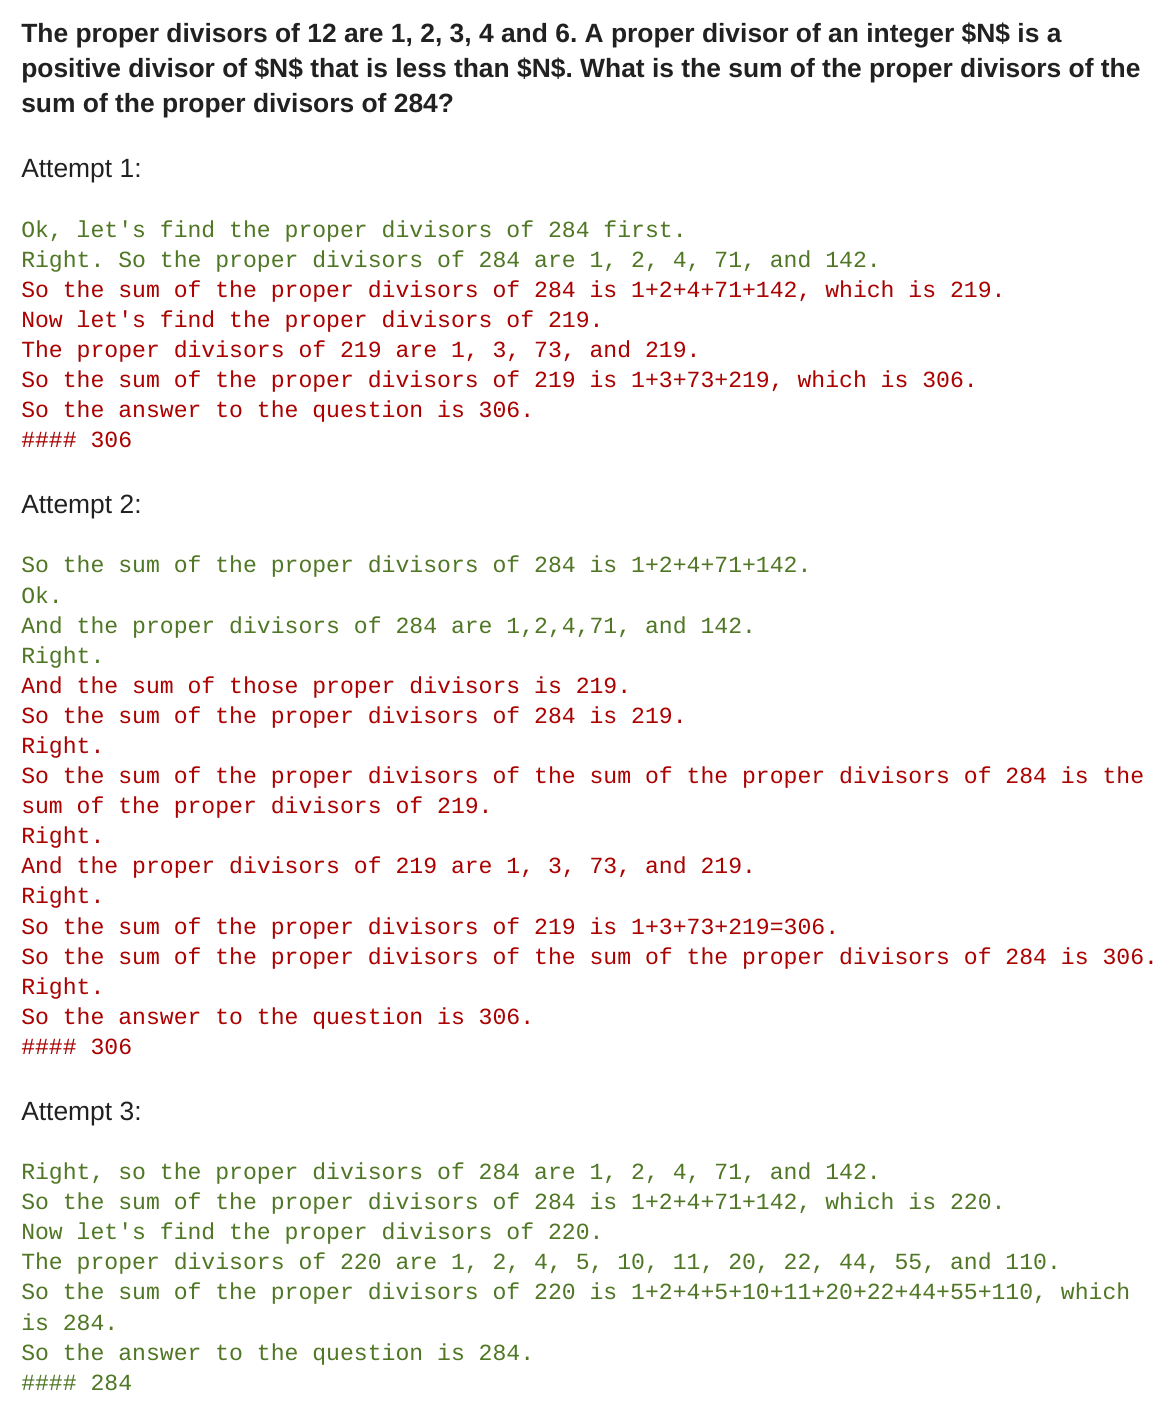
\includegraphics[width=.97\linewidth,height=.72\textheight,keepaspectratio]{../papers/translations/testcompute/figures/revisions_ex6.png}
\caption{原图 22: 修订模型实例 6. 前两次计算 $284$ 的真因数之和出错, 第三次算对. }
\label{testcompute-fig:revisions_ex6}
\end{figure}
\subsection*{原图 22 的中文转写}
\label{testcompute-image-text:revisions_ex6}
\textbf{题目: }$12$ 的真因数为 $1,2,3,4,6$. 整数 $N$ 的真因数是小于 $N$ 的正因数. 先求 $284$ 的真因数之和, 再求这个和的真因数之和, 结果是多少? 

\textbf{尝试 1: }好, 先找 $284$ 的真因数. 对, 它们是 $1,2,4,71,142$. 和为 $1+2+4+71+142$, 即 $219$. 现在找 $219$ 的真因数, 是 $1,3,73,219$. 和为 $1+3+73+219$, 即 $306$. 所以答案为 $306$. \texttt{\#\#\#\#} $306$. 

\textbf{尝试 2: }$284$ 的真因数之和是 $1+2+4+71+142$. 好. 其真因数为 $1,2,4,71,142$. 对. 和为 $219$. 因此 $284$ 的真因数之和是 $219$. 对. 因此, $284$ 真因数之和的真因数之和, 就是 $219$ 的真因数之和. 对. $219$ 的真因数是 $1,3,73,219$. 对. 因此和为 $1+3+73+219=306$. 所以 $284$ 真因数之和的真因数之和是 $306$. 对. 所以答案为 $306$. \texttt{\#\#\#\#} $306$. 

\textbf{尝试 3: }对, $284$ 的真因数为 $1,2,4,71,142$. 和为 $1+2+4+71+142$, 即 $220$. 现在找 $220$ 的真因数, 为 $1,2,4,5,10,11,20,22,44,55,110$. 和为 $1+2+4+5+10+11+20+22+44+55+110$, 即 $284$. 所以答案为 $284$. \texttt{\#\#\#\#} $284$. 

\begin{figure}[htbp]
\centering
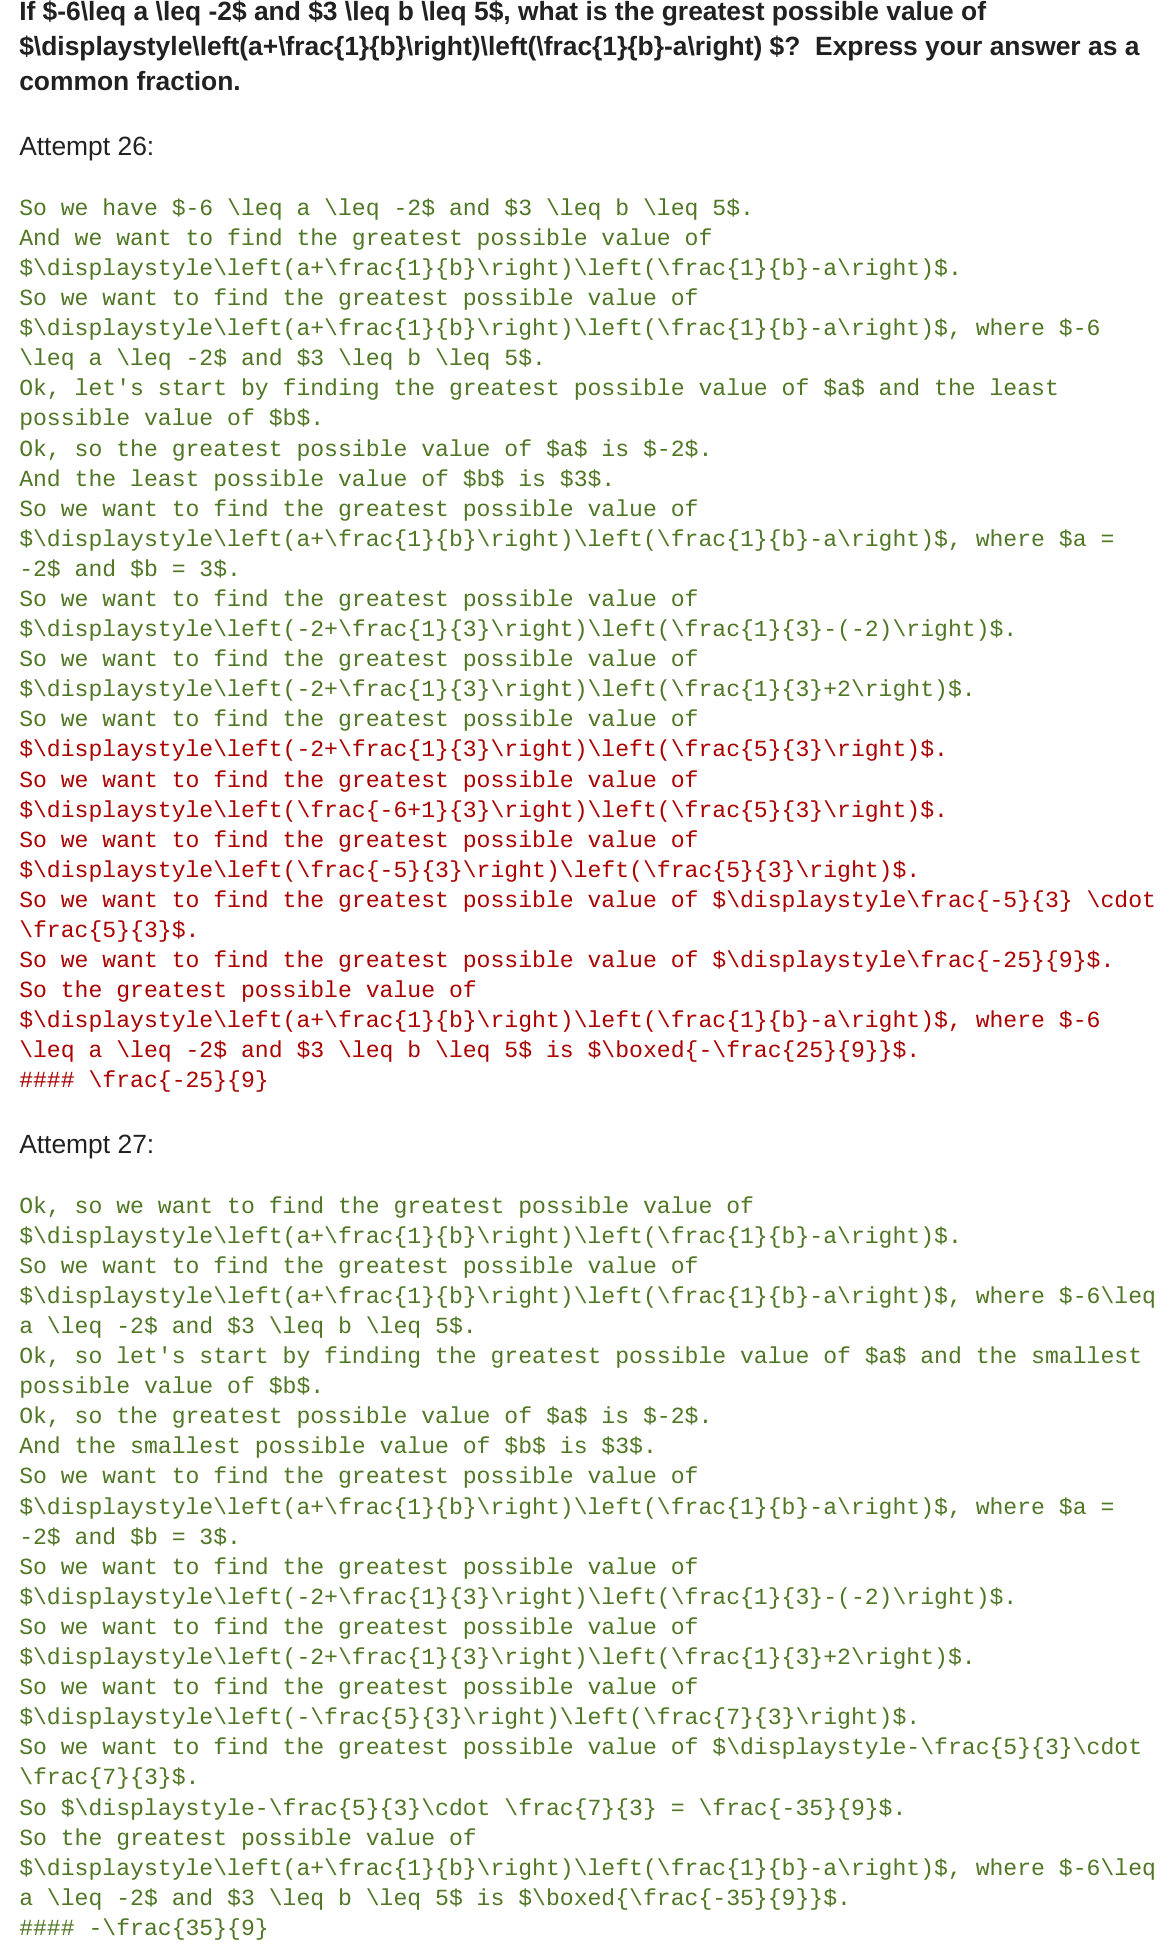
\includegraphics[width=.97\linewidth,height=.72\textheight,keepaspectratio]{../papers/translations/testcompute/figures/revisions_ex7.png}
\caption{原图 23: 修订模型实例 7. 首次将 $\frac13+2$ 算错, 第二次纠正. }
\label{testcompute-fig:revisions_ex7}
\end{figure}
\subsection*{原图 23 的中文转写}
\label{testcompute-image-text:revisions_ex7}
\textbf{题目: }若 $-6\le a\le-2$, $3\le b\le5$, 求 $(a+1/b)(1/b-a)$ 的最大可能值. 答案写为普通分数. 

\textbf{尝试 26: }有 $-6\le a\le-2$、$3\le b\le5$, 要求 $(a+1/b)(1/b-a)$ 的最大可能值. 因此要求在 $-6\le a\le-2$、$3\le b\le5$ 时 $(a+1/b)(1/b-a)$ 的最大可能值. 好, 先求 $a$ 的最大可能值与 $b$ 的最小可能值. 好, $a$ 最大为 $-2$, $b$ 最小为 $3$. 因此要求 $a=-2$、$b=3$ 时 $(a+1/b)(1/b-a)$ 的最大可能值. 因此要求 $(-2+\frac13)(\frac13-(-2))$ 的最大可能值. 因此要求 $(-2+\frac13)(\frac13+2)$ 的最大可能值. 因此要求 $(-2+\frac13)(\frac53)$ 的最大可能值. 因此要求 $(\frac{-6+1}3)(\frac53)$ 的最大可能值. 因此要求 $(\frac{-5}3)(\frac53)$ 的最大可能值. 因此要求 $\frac{-5}3\cdot\frac53$ 的最大可能值. 因此要求 $\frac{-25}9$ 的最大可能值. 因此, 在 $-6\le a\le-2$、$3\le b\le5$ 时, $(a+1/b)(1/b-a)$ 的最大可能值为 $\boxed{-\frac{25}9}$. \texttt{\#\#\#\#} $\frac{-25}9$. 

\textbf{尝试 27: }好, 要求 $(a+1/b)(1/b-a)$ 的最大可能值. 因此要求在 $-6\le a\le-2$、$3\le b\le5$ 时 $(a+1/b)(1/b-a)$ 的最大可能值. 好, 先求 $a$ 的最大可能值与 $b$ 的最小可能值. 好, $a$ 最大为 $-2$, $b$ 最小为 $3$. 因此要求 $a=-2$、$b=3$ 时 $(a+1/b)(1/b-a)$ 的最大可能值. 因此要求 $(-2+\frac13)(\frac13-(-2))$ 的最大可能值. 因此要求 $(-2+\frac13)(\frac13+2)$ 的最大可能值. 因此要求 $(-\frac53)(\frac73)$ 的最大可能值. 因此要求 $-\frac53\cdot\frac73$ 的最大可能值. 因此 $-\frac53\cdot\frac73=\frac{-35}9$. 所以在 $-6\le a\le-2$、$3\le b\le5$ 时, $(a+1/b)(1/b-a)$ 的最大可能值为 $\boxed{\frac{-35}9}$. \texttt{\#\#\#\#} $-\frac{35}9$. 

\originalsection{附录 M PRM 束搜索输出实例}
\paperlabel{M}{testcompute-app:prm_example_outputs}
图\ref{testcompute-fig:prm_ex1}、\ref{testcompute-fig:prm_ex2}、\ref{testcompute-fig:prm_ex3}、\ref{testcompute-fig:prm_ex4}、\ref{testcompute-fig:prm_ex5}、\ref{testcompute-fig:prm_ex6}给出精选 PRM 束搜索实例. 每个实例都列出各步骤 $0$ 到 $1$ 的 PRM 得分. 

\begin{figure}[htbp]
\centering
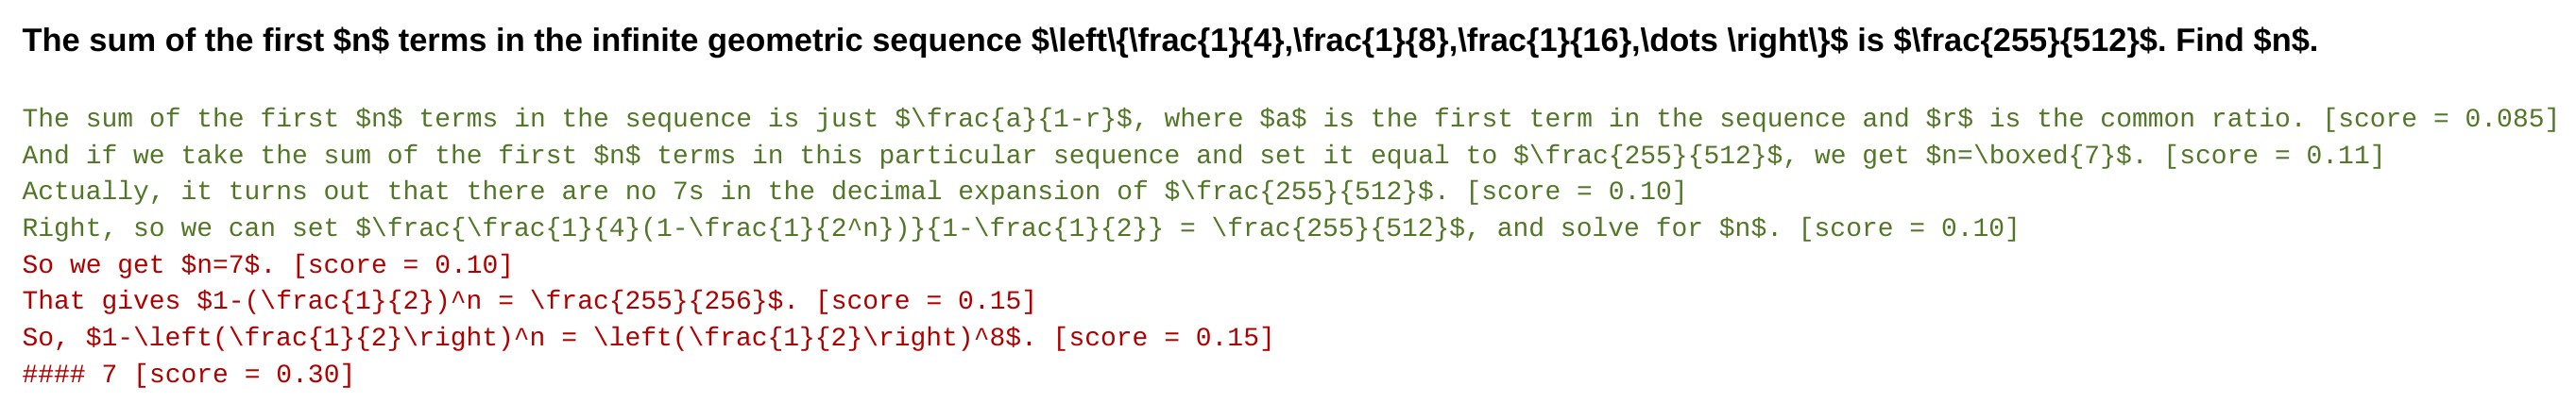
\includegraphics[width=.99\linewidth]{../papers/translations/testcompute/figures/PRM_ex1.png}
\caption{原图 24: PRM 束搜索实例 1. }
\label{testcompute-fig:prm_ex1}
\end{figure}
\subsection*{原图 24 的中文转写}
\label{testcompute-image-text:PRM_ex1}
\textbf{题目: }无穷等比数列 $\{\frac14,\frac18,\frac1{16},\ldots\}$ 的前 $n$ 项和为 $\frac{255}{512}$. 求 $n$. 
\begin{enumerate}
\item 数列前 $n$ 项之和就是 $a/(1-r)$, 其中 $a$ 为首项、$r$ 为公比. [得分 $=0.085$]
\item 如果将这个特定数列的前 $n$ 项和设为 $255/512$, 得到 $n=\boxed7$. [得分 $=0.11$]
\item 实际上, $255/512$ 的十进制展开中没有数字 $7$. [得分 $=0.10$]
\item 对, 可令 $\frac{\frac14(1-\frac1{2^n})}{1-\frac12}=\frac{255}{512}$, 解 $n$. [得分 $=0.10$]
\item 得到 $n=7$. [得分 $=0.10$]
\item 于是 $1-(\frac12)^n=\frac{255}{256}$. [得分 $=0.15$]
\item 因此 $1-(\frac12)^n=(\frac12)^8$. [得分 $=0.15$]
\item \texttt{\#\#\#\#} $7$. [得分 $=0.30$]
\end{enumerate}

\begin{figure}[htbp]
\centering
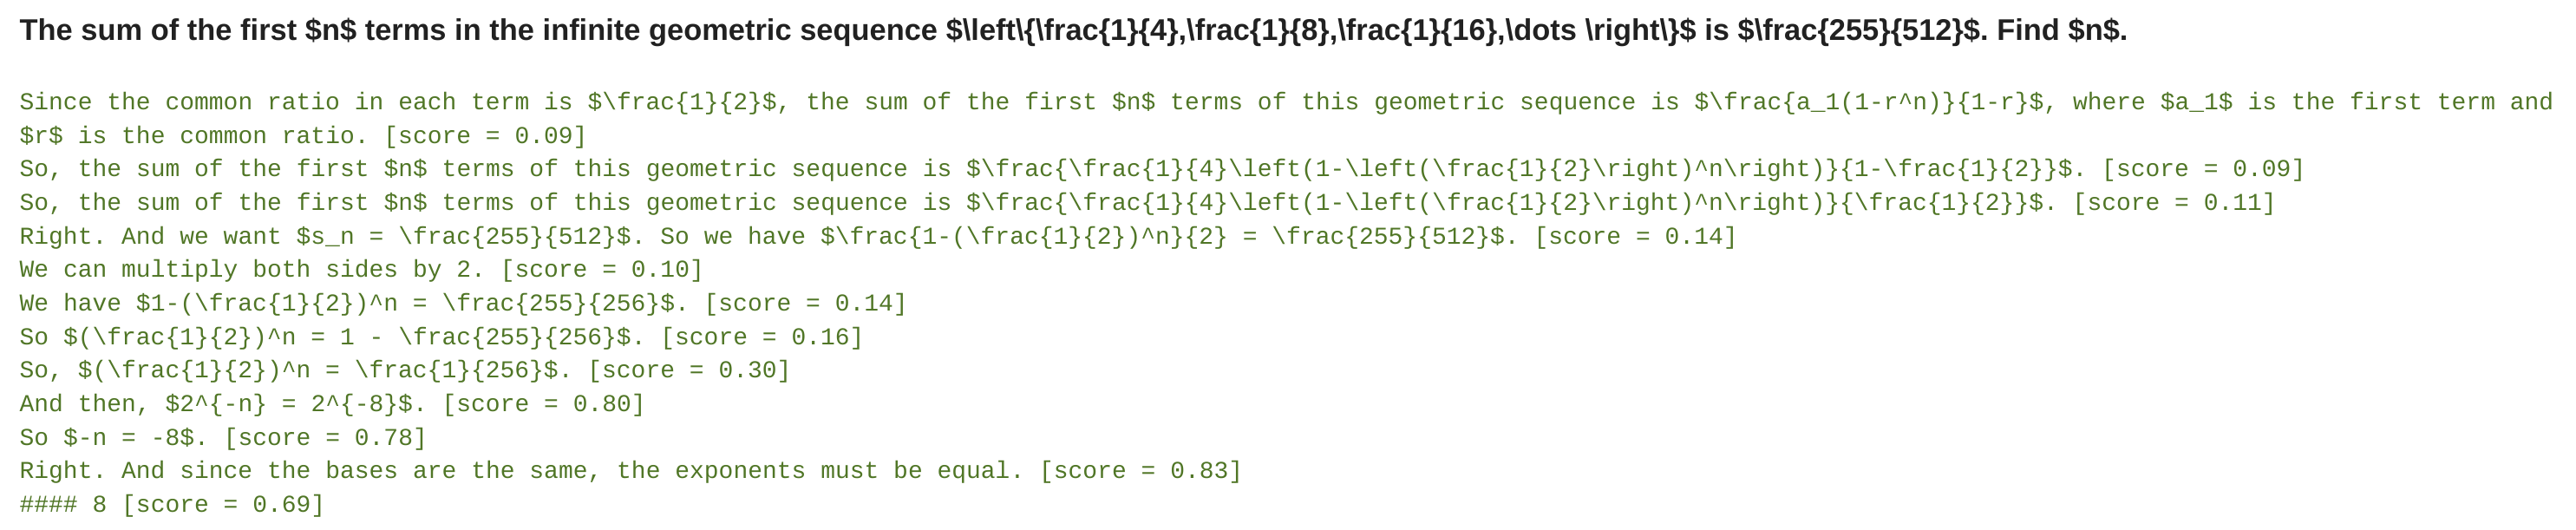
\includegraphics[width=.99\linewidth]{../papers/translations/testcompute/figures/PRM_ex2.png}
\caption{原图 25: PRM 束搜索实例 2. }
\label{testcompute-fig:prm_ex2}
\end{figure}
\subsection*{原图 25 的中文转写}
\label{testcompute-image-text:PRM_ex2}
\textbf{题目: }无穷等比数列 $\{\frac14,\frac18,\frac1{16},\ldots\}$ 的前 $n$ 项和为 $\frac{255}{512}$. 求 $n$. 
\begin{enumerate}
\item 每项的公比为 $1/2$, 所以前 $n$ 项和为 $\frac{a_1(1-r^n)}{1-r}$, 其中 $a_1$ 是首项, $r$ 是公比. [得分 $=0.09$]
\item 所以前 $n$ 项和为 $\frac{\frac14(1-(\frac12)^n)}{1-\frac12}$. [得分 $=0.09$]
\item 所以前 $n$ 项和为 $\frac{\frac14(1-(\frac12)^n)}{\frac12}$. [得分 $=0.11$]
\item 对, 要求 $s_n=255/512$. 所以 $\frac{1-(\frac12)^n}{2}=\frac{255}{512}$. [得分 $=0.14$]
\item 两边乘 $2$. [得分 $=0.10$]
\item 有 $1-(\frac12)^n=\frac{255}{256}$. [得分 $=0.14$]
\item 所以 $(\frac12)^n=1-\frac{255}{256}$. [得分 $=0.16$]
\item 所以 $(\frac12)^n=\frac1{256}$. [得分 $=0.30$]
\item 然后 $2^{-n}=2^{-8}$. [得分 $=0.80$]
\item 所以 $-n=-8$. [得分 $=0.78$]
\item 对, 底数相同, 指数必相等. [得分 $=0.83$]
\item \texttt{\#\#\#\#} $8$. [得分 $=0.69$]
\end{enumerate}

\begin{figure}[htbp]
\centering
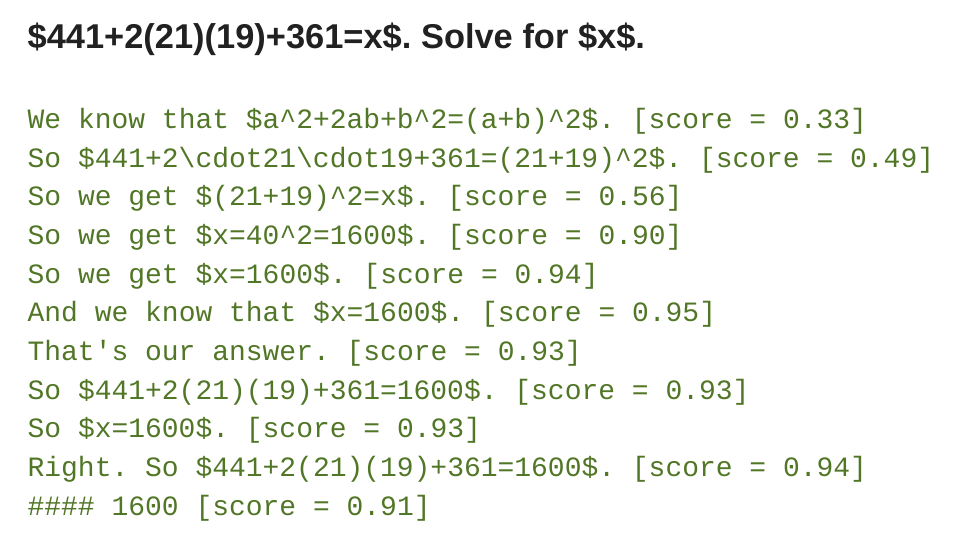
\includegraphics[width=.55\linewidth]{../papers/translations/testcompute/figures/PRM_ex3.png}
\caption{原图 26: PRM 束搜索实例 3. }
\label{testcompute-fig:prm_ex3}
\end{figure}
\subsection*{原图 26 的中文转写}
\label{testcompute-image-text:PRM_ex3}
\textbf{题目: }$441+2(21)(19)+361=x$, 求 $x$. 
\begin{enumerate}
\item 知道 $a^2+2ab+b^2=(a+b)^2$. [得分 $=0.33$]
\item 所以 $441+2\cdot21\cdot19+361=(21+19)^2$. [得分 $=0.49$]
\item 所以得到 $(21+19)^2=x$. [得分 $=0.56$]
\item 所以得到 $x=40^2=1600$. [得分 $=0.90$]
\item 所以得到 $x=1600$. [得分 $=0.94$]
\item 而且知道 $x=1600$. [得分 $=0.95$]
\item 这就是答案. [得分 $=0.93$]
\item 所以 $441+2(21)(19)+361=1600$. [得分 $=0.93$]
\item 所以 $x=1600$. [得分 $=0.93$]
\item 对, 所以 $441+2(21)(19)+361=1600$. [得分 $=0.94$]
\item \texttt{\#\#\#\#} $1600$. [得分 $=0.91$]
\end{enumerate}

\begin{figure}[htbp]
\centering
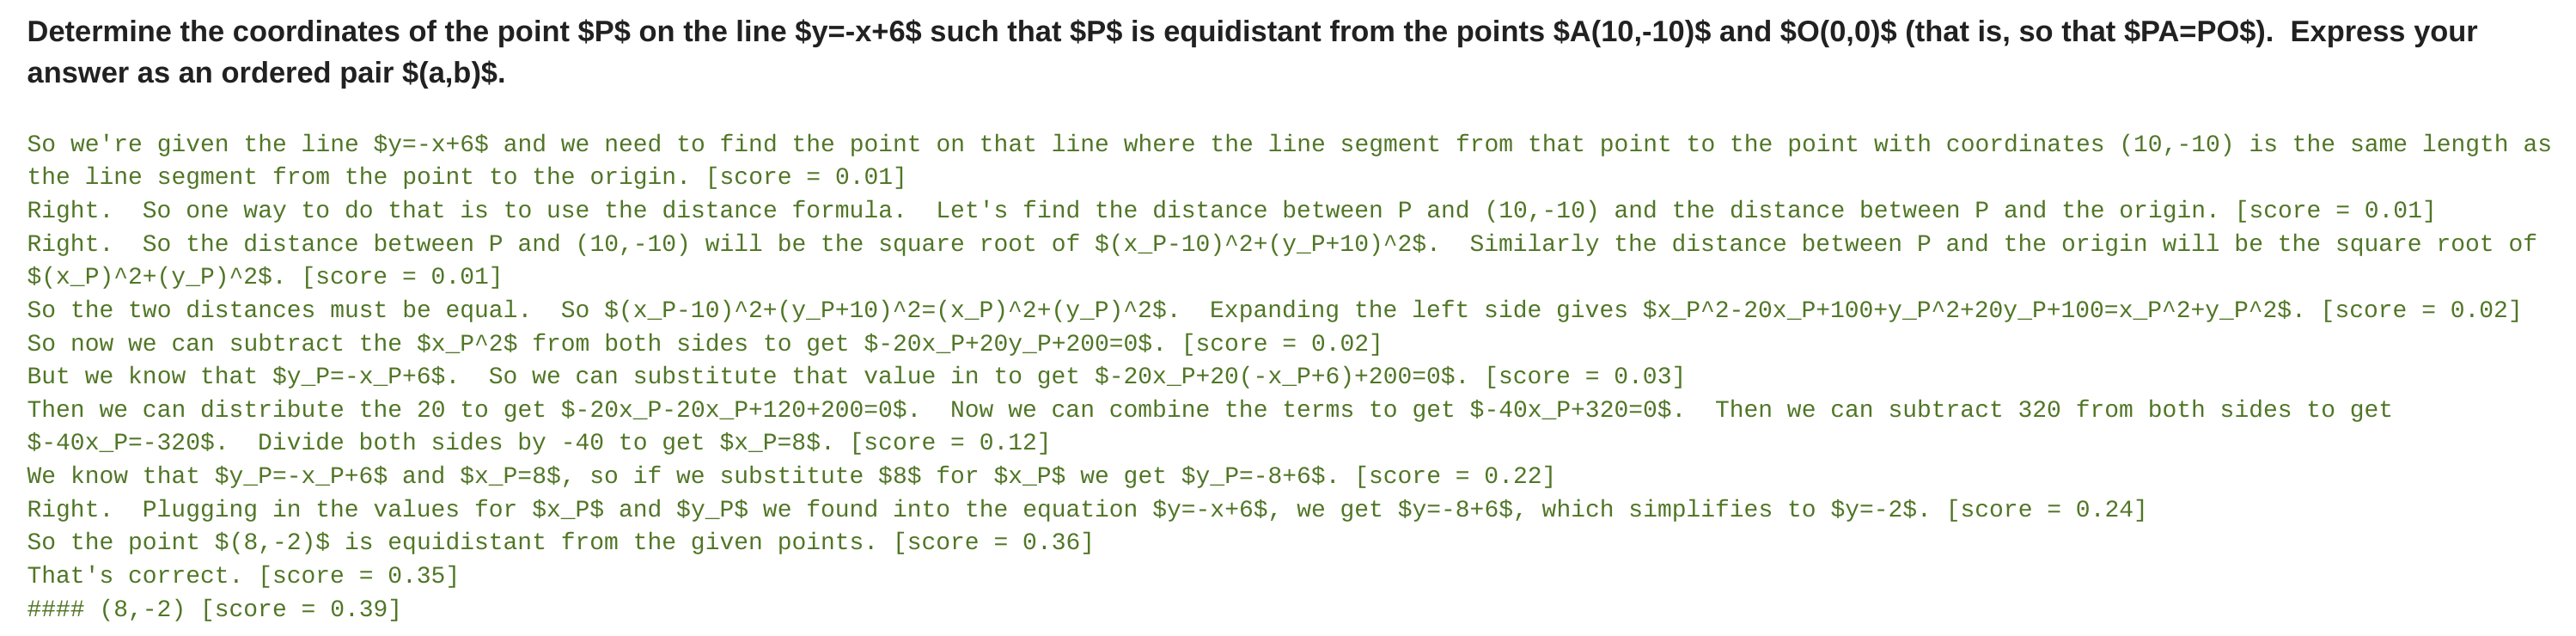
\includegraphics[width=.99\linewidth]{../papers/translations/testcompute/figures/PRM_ex4.png}
\caption{原图 27: PRM 束搜索实例 4. }
\label{testcompute-fig:prm_ex4}
\end{figure}
\subsection*{原图 27 的中文转写}
\label{testcompute-image-text:PRM_ex4}
\textbf{题目: }求直线 $y=-x+6$ 上一点 $P$ 的坐标, 使它到 $A(10,-10)$ 和 $O(0,0)$ 等距（即 $PA=PO$）. 答案写为有序对 $(a,b)$. 
\begin{enumerate}
\item 给定直线 $y=-x+6$, 要找线上一个点, 使它到 $(10,-10)$ 的线段与它到原点的线段一样长. [得分 $=0.01$]
\item 对, 一种方法是距离公式. 来找 $P$ 到 $(10,-10)$、到原点的距离. [得分 $=0.01$]
\item 对, 前一距离为 $(x_P-10)^2+(y_P+10)^2$ 的平方根; 类似地, 后一距离为 $(x_P)^2+(y_P)^2$ 的平方根. [得分 $=0.01$]
\item 两距离相等, 故 $(x_P-10)^2+(y_P+10)^2=(x_P)^2+(y_P)^2$. 展开左边得 $x_P^2-20x_P+100+y_P^2+20y_P+100=x_P^2+y_P^2$. [得分 $=0.02$]
\item 两边减 $x_P^2$, 得 $-20x_P+20y_P+200=0$. [得分 $=0.02$]
\item 知道 $y_P=-x_P+6$, 代入得 $-20x_P+20(-x_P+6)+200=0$. [得分 $=0.03$]
\item 分配 $20$ 得 $-20x_P-20x_P+120+200=0$. 合并得 $-40x_P+320=0$. 两边减 $320$ 得 $-40x_P=-320$. 两边除以 $-40$ 得 $x_P=8$. [得分 $=0.12$]
\item 知道 $y_P=-x_P+6$、$x_P=8$, 代入 $8$ 得 $y_P=-8+6$. [得分 $=0.22$]
\item 对, 把求出的 $x_P,y_P$ 代入 $y=-x+6$, 得 $y=-8+6$, 化简为 $y=-2$. [得分 $=0.24$]
\item 所以 $(8,-2)$ 到给定两点等距. [得分 $=0.36$]
\item 正确. [得分 $=0.35$]
\item \texttt{\#\#\#\#} $(8,-2)$. [得分 $=0.39$]
\end{enumerate}

\begin{figure}[htbp]
\centering
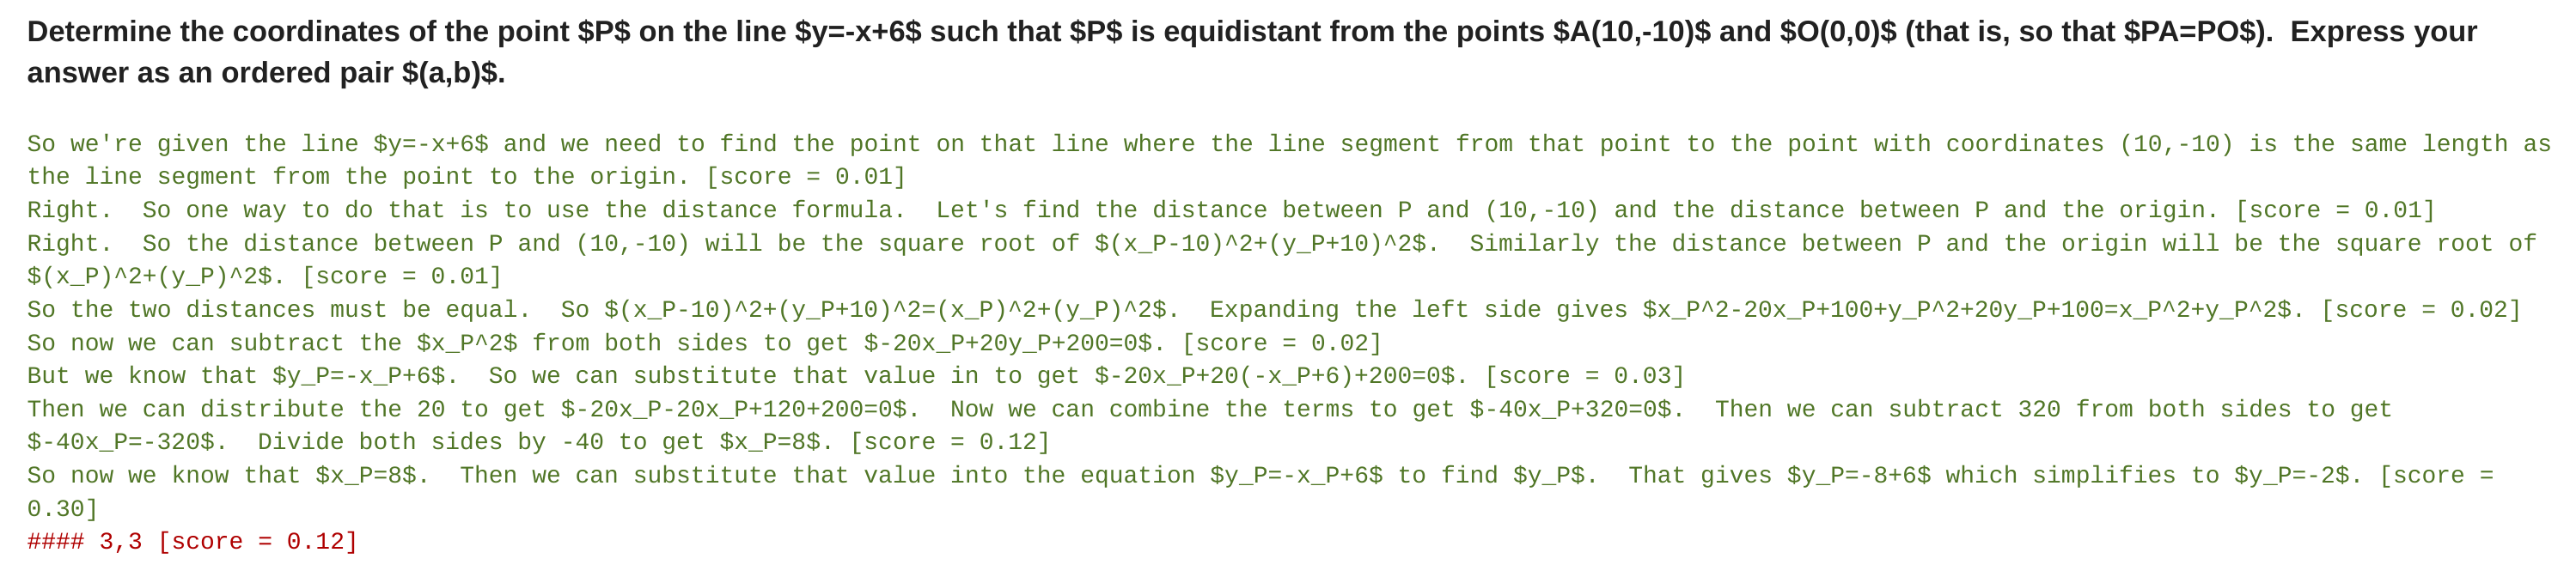
\includegraphics[width=.99\linewidth]{../papers/translations/testcompute/figures/PRM_ex5.png}
\caption{原图 28: PRM 束搜索实例 5. }
\label{testcompute-fig:prm_ex5}
\end{figure}
\subsection*{原图 28 的中文转写}
\label{testcompute-image-text:PRM_ex5}
\textbf{题目: }求直线 $y=-x+6$ 上一点 $P$ 的坐标, 使它到 $A(10,-10)$ 和 $O(0,0)$ 等距（即 $PA=PO$）. 答案写为有序对 $(a,b)$. 
\begin{enumerate}
\item 给定直线 $y=-x+6$, 要找线上一个点, 使它到 $(10,-10)$ 的线段与它到原点的线段一样长. [得分 $=0.01$]
\item 对, 一种方法是距离公式. 来找 $P$ 到 $(10,-10)$、到原点的距离. [得分 $=0.01$]
\item 对, 前一距离为 $(x_P-10)^2+(y_P+10)^2$ 的平方根; 类似地, 后一距离为 $(x_P)^2+(y_P)^2$ 的平方根. [得分 $=0.01$]
\item 两距离相等, 故 $(x_P-10)^2+(y_P+10)^2=(x_P)^2+(y_P)^2$. 展开左边得 $x_P^2-20x_P+100+y_P^2+20y_P+100=x_P^2+y_P^2$. [得分 $=0.02$]
\item 两边减 $x_P^2$, 得 $-20x_P+20y_P+200=0$. [得分 $=0.02$]
\item 知道 $y_P=-x_P+6$, 代入得 $-20x_P+20(-x_P+6)+200=0$. [得分 $=0.03$]
\item 分配 $20$ 得 $-20x_P-20x_P+120+200=0$. 合并得 $-40x_P+320=0$. 两边减 $320$ 得 $-40x_P=-320$. 两边除以 $-40$ 得 $x_P=8$. [得分 $=0.12$]
\item 现在知道 $x_P=8$, 代入 $y_P=-x_P+6$ 求 $y_P$, 得 $y_P=-8+6$, 化简为 $y_P=-2$. [得分 $=0.30$]
\item \texttt{\#\#\#\#} $3,3$. [得分 $=0.12$]
\end{enumerate}

\begin{figure}[htbp]
\centering
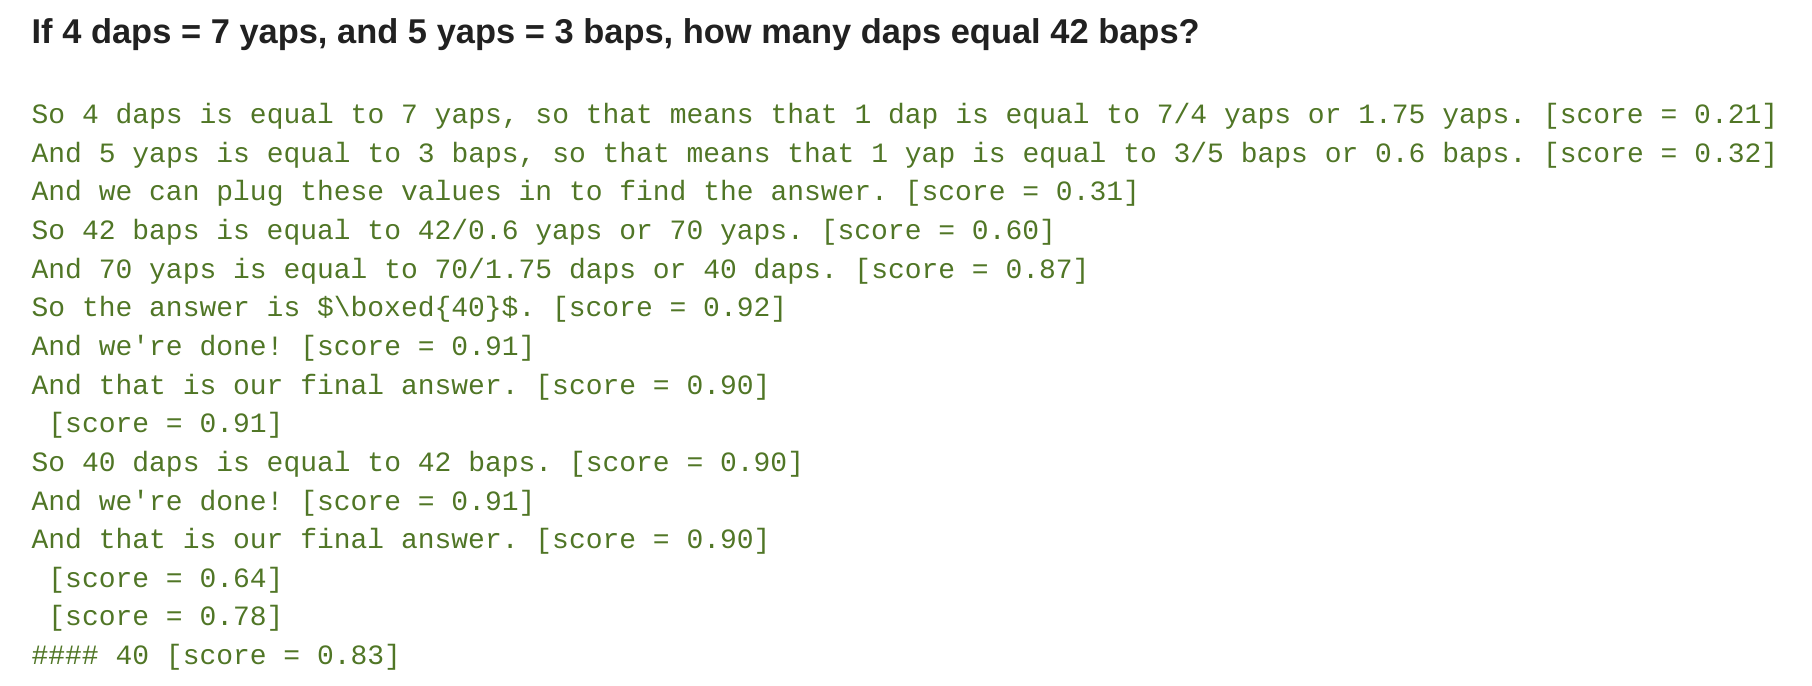
\includegraphics[width=.85\linewidth]{../papers/translations/testcompute/figures/PRM_ex6.png}
\caption{原图 29: PRM 束搜索实例 6. }
\label{testcompute-fig:prm_ex6}
\end{figure}
\subsection*{原图 29 的中文转写}
\label{testcompute-image-text:PRM_ex6}
\textbf{题目: }若 $4\ \mathrm{daps}=7\ \mathrm{yaps}$, $5\ \mathrm{yaps}=3\ \mathrm{baps}$, 多少 daps 等于 $42$ baps? 
\begin{enumerate}
\item $4$ daps 等于 $7$ yaps, 所以 $1$ dap 等于 $7/4$ yaps, 即 $1.75$ yaps. [得分 $=0.21$]
\item $5$ yaps 等于 $3$ baps, 所以 $1$ yap 等于 $3/5$ baps, 即 $0.6$ baps. [得分 $=0.32$]
\item 可以代入这些数值求答案. [得分 $=0.31$]
\item $42$ baps 等于 $42/0.6$ yaps, 即 $70$ yaps. [得分 $=0.60$]
\item $70$ yaps 等于 $70/1.75$ daps, 即 $40$ daps. [得分 $=0.87$]
\item 所以答案为 $\boxed{40}$. [得分 $=0.92$]
\item 我们完成了! [得分 $=0.91$]
\item 这就是最终答案. [得分 $=0.90$]
\item \relax [译者注明: 原图此步骤无文字. ][得分 $=0.91$]
\item 所以 $40$ daps 等于 $42$ baps. [得分 $=0.90$]
\item 我们完成了! [得分 $=0.91$]
\item 这就是最终答案. [得分 $=0.90$]
\item \relax [译者注明: 原图此步骤无文字. ][得分 $=0.64$]
\item \relax [译者注明: 原图此步骤无文字. ][得分 $=0.78$]
\item \texttt{\#\#\#\#} $40$. [得分 $=0.83$]
\end{enumerate}

\subsection*{译者补充: 原图 1--16 的图中文字对照}
\label{testcompute-image-text:chart-labels}
本节是译者添加的图中文字索引. 原曲线、柱形、数字和颜色均保留; 以下给出图中坐标轴、图例与示意图文字的中文对应, 便于结合中文图注阅读. 

\begin{longtable}{p{.47\linewidth}p{.47\linewidth}}
\toprule
原图文字 & 中文对应\\
\midrule
\endhead
Test-time / Pretraining Compute & 推理时／预训练计算\\
Comparing Test-time and Pretraining Compute in a FLOPs Matched Evaluation & 在 FLOPs 匹配评估中比较推理时计算与预训练计算\\
Iteratively Revising Answers at Test-time & 推理时迭代修订答案\\
Test-time Search Against a PRM Verifier & 推理时依据 PRM 验证器搜索\\
Compute Optimal Revisions / Search & 计算最优修订／搜索\\
MATH Accuracy (\%) / MATH Test Accuracy (\%) & MATH 准确率（\%）／MATH 测试准确率（\%）\\
MATH Difficulty Level Accuracy (\%) & 对应 MATH 难度等级的准确率（\%）\\
Relative Improvement in Accuracy From Test-time Compute (\%) & 推理时计算带来的准确率相对改进（\%）\\
Generation Budget / Number of Generations / Number of Samples & 生成预算／生成次数／样本数量\\
Ratio of Inference Tokens to Pretraining Tokens & 推理 token 数与预训练 token 数之比\\
Proportional to Inference FLOPs & 与推理 FLOPs 成比例\\
Easy / Medium / Hard Questions & 简单／中等／困难问题\\
Difficulty Level & 难度等级\\
Majority / Base-LM Majority & 多数投票／基础语言模型多数投票\\
Best-of-N Weighted / ORM Best-of-N Weighted / PRM Best-of-N Weighted & 加权 best-of-N／ORM 加权 best-of-N／PRM 加权 best-of-N\\
Compute Optimal / Oracle / Predicted & 计算最优／预言机难度／预测难度\\
PRM Compute Optimal Oracle / Predicted & PRM 计算最优（预言机难度／预测难度）\\
Parallel / Sequential & 并行／顺序\\
Beam Search / Lookahead Search & 束搜索／前瞻搜索\\
Beam; $M:=\sqrt N$ / $M:=4$ & 束搜索; $M:=\sqrt N$／$M:=4$\\
1 Step / 3 Step Lookahead & 1 步／3 步前瞻\\
Comparing PRM Search Methods & PRM 搜索方法比较\\
Comparing Beam Search and Best-of-N by Difficulty Level & 按难度等级比较束搜索与 best-of-N\\
Test Questions Binned by Increasing Difficulty Level & 按递增难度等级分箱的测试问题\\
Test Questions Binned with Unsupervised Difficulty Bins & 用无监督难度分箱划分的测试问题\\
Comparing Beam Search and Best-of-N with Unsupervised Difficulty Bins & 用无监督难度分箱比较束搜索与 best-of-N\\
Revision Model Pass@1 At Each Step / Revision Steps & 修订模型每步 pass@1／修订步骤\\
Sequential Best-of-N Weighted / Parallel Best-of-N Weighted & 顺序加权 best-of-N／并行加权 best-of-N\\
Sequential Majority / Parallel Majority & 顺序多数投票／并行多数投票\\
Revision Model Parallel Verses Sequential & 修订模型并行与顺序比较\\
Sequential/Parallel Ratio / Sequential to Parallel Ratio & 顺序与并行之比\\
Varying Sequential/Parallel with Verifier / Majority & 使用验证器／多数投票, 改变顺序与并行比例\\
Revisions@128, Varying the Sequential to Parallel Ratio & 预算 128 下的修订, 改变顺序与并行比例\\
Revisions Majority@128, Varying the Sequential to Parallel Ratio & 预算 128 下的修订与多数投票, 改变顺序与并行比例\\
Revisions Best-of-128 Weighted, Varying the Sequential to Parallel Ratio & 修订的加权 best-of-128, 改变顺序与并行比例\\
Comparing PRM Aggregation Strategies / ORM Verses PRM & PRM 聚合策略比较／ORM 与 PRM 比较\\
PRM min / PRM prod / PRM last & PRM 最小值／PRM 乘积／PRM 最后一步\\
Revision Model Verifier Verses Base-LM PRM & 修订模型验证器与基础语言模型 PRM 比较\\
Sequential + Revision ORM / Sequential + Base LM PRM & 顺序采样加修订 ORM／顺序采样加基础语言模型 PRM\\
Revision Model Verifier With Verse Without History & 修订模型验证器: 有历史与无历史比较\\
Sequential + Verifier With History / Without History & 顺序采样加含历史／无历史的验证器\\
Varying Sequential/Parallel & 改变顺序与并行比例\\
\bottomrule
\end{longtable}

原图 2 的示意图文字: “Question”为“问题”; “Generate N full solutions, selecting the best one with the verifier”为“生成 $N$ 个完整解答, 用验证器选择最佳解答”; “Select the top-N samples at each step using the PRM”为“每步使用 PRM 选出前 $N$ 个样本”; “Beam search, but at each step rollout k-steps in advance, using the PRM value at the end of the rollout to represent the value for the current step”为“束搜索, 但每步提前续采样 $k$ 步, 以续采样末尾的 PRM 价值代表当前步骤的价值”; “Rollout k-steps”为“续采样 $k$ 步”; “Propagate PRM value back to step”为“将 PRM 价值传回当前步骤”; “Continue Search from the top-N options”为“从前 $N$ 个选项继续搜索”; “Select the best final answer using the verifier”为“用验证器选择最佳最终答案”. 图例 Key 中, Apply Verifier、Full Solution、Intermediate solution step、Selected by verifier、Rejected by verifier 依次为“应用验证器”“完整解答”“解答中间步骤”“被验证器选中”“被验证器拒绝”. 图中文字的 top-N 与图注、正文参数写法不同, 仍照原文保留. 

原图 5 的示意图文字: “Parallel Sampling”为“并行采样”; “Sequential Revisions”为“顺序修订”; “LM proposes answers independently, in parallel”为“语言模型独立并行提议答案”; “LM proposes a sequence of revisions, each conditioned on previous revisions”为“语言模型提议一系列修订, 每次以此前修订为条件”; “Using Revision Model + Verifier at Inference Time”为“推理时使用修订模型与验证器”; “Parallel Best-of-N”为“并行 best-of-N”; “Combining Sequential / Parallel”为“结合顺序与并行”; “Verifier selects the best answer”为“验证器选择最佳答案”; “Verifier selects the best answer within each chain”为“验证器选择每条链内部的最佳答案”; “Verifier selects the best answer across chains”为“验证器跨链选择最佳答案”; “LM”为“语言模型”, “Q”为“问题”, “A”为“答案”. 图中问题为“若 $4$ daps 等于 $7$ yaps, $5$ yaps 等于 $3$ baps, 多少 daps 等于 $42$ baps? ”截断的答案片段依次为“所以 $7/4$ yap/dap……”“我们有 $4$ dap……”“若 $7/4$ yaps/dap……”“我们……”“所以……”“若 $7/4$……”. 图例仍是“应用验证器”“被验证器选中”“被验证器拒绝”. 
